% ----------------------------------------------------------------------
%
%                            TFMTesis.tex
%
%----------------------------------------------------------------------
%
% Este fichero contiene el "documento maestro" del documento. Lo único
% que hace es configurar el entorno LaTeX e incluir los ficheros .tex
% que contienen cada sección.
%
%----------------------------------------------------------------------
%
% Los ficheros necesarios para este documento son:
%
%       TeXiS/* : ficheros de la plantilla TeXiS.
%       Cascaras/* : ficheros con las partes del documento que no
%          son capítulos ni apéndices (portada, agradecimientos, etc.)
%       Capitulos/*.tex : capítulos de la tesis
%       Apendices/*.tex: apéndices de la tesis
%       constantes.tex: constantes LaTeX
%       config.tex : configuración de la "compilación" del documento
%       guionado.tex : palabras con guiones
%
% Para la bibliografía, además, se necesitan:
%
%       *.bib : ficheros con la información de las referencias
%
% ---------------------------------------------------------------------

\documentclass[12pt,a4paper,twoside]{book}

%
% Definimos  el   comando  \compilaCapitulo,  que   luego  se  utiliza
% (opcionalmente) en config.tex. Quedaría  mejor si también se definiera
% en  ese fichero,  pero por  el modo  en el  que funciona  eso  no es
% posible. Puedes consultar la documentación de ese fichero para tener
% más  información. Definimos también  \compilaApendice, que  tiene el
% mismo  cometido, pero  que se  utiliza para  compilar  únicamente un
% apéndice.
%
%
% Si  queremos   compilar  solo   una  parte  del   documento  podemos
% especificar mediante  \includeonly{...} qué ficheros  son los únicos
% que queremos  que se incluyan.  Esto  es útil por  ejemplo para sólo
% compilar un capítulo.
%
% El problema es que todos aquellos  ficheros que NO estén en la lista
% NO   se  incluirán...  y   eso  también   afecta  a   ficheros  de
% la plantilla...
%
% Total,  que definimos  una constante  con los  ficheros  que siempre
% vamos a querer compilar  (aquellos relacionados con configuración) y
% luego definimos \compilaCapitulo.
\newcommand{\ficherosBasicosTeXiS}{%
TeXiS/TeXiS_pream,TeXiS/TeXiS_cab,TeXiS/TeXiS_bib,TeXiS/TeXiS_cover%
}
\newcommand{\ficherosBasicosTexto}{%
constantes,guionado,Cascaras/bibliografia,config%
}
\newcommand{\compilaCapitulo}[1]{%
\includeonly{\ficherosBasicosTeXiS,\ficherosBasicosTexto,Capitulos/#1}%
}

\newcommand{\compilaApendice}[1]{%
\includeonly{\ficherosBasicosTeXiS,\ficherosBasicosTexto,Apendices/#1}%
}

%- - - - - - - - - - - - - - - - - - - - - - - - - - - - - - - - - - -
%            Preámbulo del documento. Configuraciones varias
%- - - - - - - - - - - - - - - - - - - - - - - - - - - - - - - - - - -

% Define  el  tipo  de  compilación que  estamos  haciendo.   Contiene
% definiciones  de  constantes que  cambian  el  comportamiento de  la
% compilación. Debe incluirse antes del paquete TeXiS/TeXiS.sty
%---------------------------------------------------------------------
%
%                          config.tex
%
%---------------------------------------------------------------------
%
% Contiene la  definición de constantes  que determinan el modo  en el
% que se compilará el documento.
%
%---------------------------------------------------------------------
%
% En concreto, podemos  indicar si queremos "modo release",  en el que
% no  aparecerán  los  comentarios  (creados  mediante  \com{Texto}  o
% \comp{Texto}) ni los "por  hacer" (creados mediante \todo{Texto}), y
% sí aparecerán los índices. El modo "debug" (o mejor dicho en modo no
% "release" muestra los índices  (construirlos lleva tiempo y son poco
% útiles  salvo  para   la  versión  final),  pero  sí   el  resto  de
% anotaciones.
%
% Si se compila con LaTeX (no  con pdflatex) en modo Debug, también se
% muestran en una esquina de cada página las entradas (en el índice de
% palabras) que referencian  a dicha página (consulta TeXiS_pream.tex,
% en la parte referente a show).
%
% El soporte para  el índice de palabras en  TeXiS es embrionario, por
% lo  que no  asumas que  esto funcionará  correctamente.  Consulta la
% documentación al respecto en TeXiS_pream.tex.
%
%
% También  aquí configuramos  si queremos  o  no que  se incluyan  los
% acrónimos  en el  documento final  en la  versión release.  Para eso
% define (o no) la constante \acronimosEnRelease.
%
% Utilizando \compilaCapitulo{nombre}  podemos también especificar qué
% capítulo(s) queremos que se compilen. Si no se pone nada, se compila
% el documento  completo.  Si se pone, por  ejemplo, 01Introduccion se
% compilará únicamente el fichero Capitulos/01Introduccion.tex
%
% Para compilar varios  capítulos, se separan sus nombres  con comas y
% no se ponen espacios de separación.
%
% En realidad  la macro \compilaCapitulo  está definida en  el fichero
% principal tesis.tex.
%
%---------------------------------------------------------------------


% Comentar la línea si no se compila en modo release.
% TeXiS hará el resto.
% ¡¡¡Si cambias esto, haz un make clean antes de recompilar!!!
\def\release{1}


% Descomentar la linea si se quieren incluir los
% acrónimos en modo release (en modo debug
% no se incluirán nunca).
% ¡¡¡Si cambias esto, haz un make clean antes de recompilar!!!
%\def\acronimosEnRelease{1}


% Descomentar la línea para establecer el capítulo que queremos
% compilar

% \compilaCapitulo{01Introduccion}
% \compilaCapitulo{02EstructuraYGeneracion}
% \compilaCapitulo{03Edicion}
% \compilaCapitulo{04Imagenes}
% \compilaCapitulo{05Bibliografia}
% \compilaCapitulo{06Makefile}

% \compilaApendice{01AsiSeHizo}

% Variable local para emacs, para  que encuentre el fichero maestro de
% compilación y funcionen mejor algunas teclas rápidas de AucTeX
%%%
%%% Local Variables:
%%% mode: latex
%%% TeX-master: "./Tesis.tex"
%%% End:


% Paquete de la plantilla
\usepackage{TeXiS/TeXiS}

% Incluimos el fichero con comandos de constantes
%---------------------------------------------------------------------
%
%                          constantes.tex
%
%---------------------------------------------------------------------
%
% Fichero que  declara nuevos comandos LaTeX  sencillos realizados por
% comodidad en la escritura de determinadas palabras
%
%---------------------------------------------------------------------

%%%%%%%%%%%%%%%%%%%%%%%%%%%%%%%%%%%%%%%%%%%%%%%%%%%%%%%%%%%%%%%%%%%%%%
% Comando: 
%
%       \titulo
%
% Resultado: 
%
% Escribe el título del documento.
%%%%%%%%%%%%%%%%%%%%%%%%%%%%%%%%%%%%%%%%%%%%%%%%%%%%%%%%%%%%%%%%%%%%%%
\def\titulo{\textsc{TeXiS}: Una plantilla de \LaTeX\
  para Tesis y otros documentos}

%%%%%%%%%%%%%%%%%%%%%%%%%%%%%%%%%%%%%%%%%%%%%%%%%%%%%%%%%%%%%%%%%%%%%%
% Comando: 
%
%       \autor
%
% Resultado: 
%
% Escribe el autor del documento.
%%%%%%%%%%%%%%%%%%%%%%%%%%%%%%%%%%%%%%%%%%%%%%%%%%%%%%%%%%%%%%%%%%%%%%
\def\autor{Marco Antonio y Pedro Pablo G\'omez Mart\'in}

% Variable local para emacs, para  que encuentre el fichero maestro de
% compilación y funcionen mejor algunas teclas rápidas de AucTeX

%%%
%%% Local Variables:
%%% mode: latex
%%% TeX-master: "tesis.tex"
%%% End:


% Sacamos en el log de la compilación el copyright
%\typeout{Copyright Marco Antonio and Pedro Pablo Gomez Martin}

%
% "Metadatos" para el PDF
%
\ifpdf\hypersetup{%
    pdftitle = {\titulo},
    pdfsubject = {Trabajo de Fin de Grado},
    pdfkeywords = {Trabajo de Fin de Grado, RPG, motor de videojuegos, videojuegos, editor de videojuegos},
    pdfauthor = {\textcopyright\ \autor},
    pdfcreator = {\LaTeX\ con el paquete \flqq hyperref\frqq},
    pdfproducer = {pdfeTeX-0.\the\pdftexversion\pdftexrevision},
    }
    \pdfinfo{/CreationDate (\today)}
\fi


%- - - - - - - - - - - - - - - - - - - - - - - - - - - - - - - - - - -
%                        Documento
%- - - - - - - - - - - - - - - - - - - - - - - - - - - - - - - - - - -
\begin{document}

% Incluimos el  fichero de definición de guionado  de algunas palabras
% que LaTeX no ha dividido como debería
%----------------------------------------------------------------
%
%                          guionado.tex
%
%----------------------------------------------------------------
%
% Fichero con algunas divisiones de palabras que LaTeX no
% hace correctamente si no se le da alguna ayuda.
%
%----------------------------------------------------------------

\hyphenation{
% a
abs-trac-to
abs-trac-tos
abs-trac-ta
abs-trac-tas
ac-tua-do-res
a-gra-de-ci-mien-tos
ana-li-za-dor
an-te-rio-res
an-te-rior-men-te
apa-rien-cia
a-pro-pia-do
a-pro-pia-dos
a-pro-pia-da
a-pro-pia-das
a-pro-ve-cha-mien-to
a-que-llo
a-que-llos
a-que-lla
a-que-llas
a-sig-na-tu-ra
a-sig-na-tu-ras
a-so-cia-da
a-so-cia-das
a-so-cia-do
a-so-cia-dos
au-to-ma-ti-za-do
% b
batch
bi-blio-gra-fía
bi-blio-grá-fi-cas
bien
bo-rra-dor
boo-l-ean-expr
% c
ca-be-ce-ra
call-me-thod-ins-truc-tion
cas-te-lla-no
cir-cuns-tan-cia
cir-cuns-tan-cias
co-he-ren-te
co-he-ren-tes
co-he-ren-cia
co-li-bri
co-men-ta-rio
co-mer-cia-les
co-no-ci-mien-to
cons-cien-te
con-si-de-ra-ba
con-si-de-ra-mos
con-si-de-rar-se
cons-tan-te
cons-trucción
cons-tru-ye
cons-tru-ir-se
con-tro-le
co-rrec-ta-men-te
co-rres-pon-den
co-rres-pon-dien-te
co-rres-pon-dien-tes
co-ti-dia-na
co-ti-dia-no
crean
cris-ta-li-zan
cu-rri-cu-la
cu-rri-cu-lum
cu-rri-cu-lar
cu-rri-cu-la-res
% d
de-di-ca-do
de-di-ca-dos
de-di-ca-da
de-di-ca-das
de-rro-te-ro
de-rro-te-ros
de-sa-rro-llo
de-sa-rro-llos
de-sa-rro-lla-do
de-sa-rro-lla-dos
de-sa-rro-lla-da
de-sa-rro-lla-das
de-sa-rro-lla-dor
de-sa-rro-llar
des-cri-bi-re-mos
des-crip-ción
des-crip-cio-nes
des-cri-to
des-pués
de-ta-lla-do
de-ta-lla-dos
de-ta-lla-da
de-ta-lla-das
di-a-gra-ma
di-a-gra-mas
di-se-ños
dis-po-ner
dis-po-ni-bi-li-dad
do-cu-men-ta-da
do-cu-men-to
do-cu-men-tos
% e
edi-ta-do
e-du-ca-ti-vo
e-du-ca-ti-vos
e-du-ca-ti-va
e-du-ca-ti-vas
e-la-bo-ra-do
e-la-bo-ra-dos
e-la-bo-ra-da
e-la-bo-ra-das
es-co-llo
es-co-llos
es-tu-dia-do
es-tu-dia-dos
es-tu-dia-da
es-tu-dia-das
es-tu-dian-te
e-va-lua-cio-nes
e-va-lua-do-res
exis-ten-tes
exhaus-ti-va
ex-pe-rien-cia
ex-pe-rien-cias
% f
for-ma-li-za-do
% g
ge-ne-ra-ción
ge-ne-ra-dor
ge-ne-ra-do-res
ge-ne-ran
% h
he-rra-mien-ta
he-rra-mien-tas
% i
i-dio-ma
i-dio-mas
im-pres-cin-di-ble
im-pres-cin-di-bles
in-de-xa-do
in-de-xa-dos
in-de-xa-da
in-de-xa-das
in-di-vi-dual
in-fe-ren-cia
in-fe-ren-cias
in-for-ma-ti-ca
in-gre-dien-te
in-gre-dien-tes
in-me-dia-ta-men-te
ins-ta-la-do
ins-tan-cias
in-te-rac-ción
% j
% k
% l
len-gua-je
li-be-ra-to-rio
li-be-ra-to-rios
li-be-ra-to-ria
li-be-ra-to-rias
li-mi-ta-do
li-te-ra-rio
li-te-ra-rios
li-te-ra-ria
li-te-ra-rias
lo-tes
% m
ma-ne-ra
ma-nual
mas-que-ra-de
ma-yor
me-mo-ria
mi-nis-te-rio
mi-nis-te-rios
mo-de-lo
mo-de-los
mo-de-la-do
mo-du-la-ri-dad
mo-vi-mien-to
% n
na-tu-ral
ni-vel
nues-tro
% o
obs-tan-te
o-rien-ta-do
o-rien-ta-dos
o-rien-ta-da
o-rien-ta-das
% p
pa-ra-le-lo
pa-ra-le-la
par-ti-cu-lar
par-ti-cu-lar-men-te
pe-da-gó-gi-ca
pe-da-gó-gi-cas
pe-da-gó-gi-co
pe-da-gó-gi-cos
pe-rio-di-ci-dad
per-so-na-je
plan-te-a-mien-to
plan-te-a-mien-tos
po-si-ción
pre-fe-ren-cia
pre-fe-ren-cias
pres-cin-di-ble
pres-cin-di-bles
pri-me-ra
pro-ble-ma
pro-ble-mas
pró-xi-mo
pu-bli-ca-cio-nes
pu-bli-ca-do
% q
% r
rá-pi-da
rá-pi-do
ra-zo-na-mien-to
ra-zo-na-mien-tos
re-a-li-zan-do
re-fe-ren-cia
re-fe-ren-cias
re-fe-ren-cia-da
re-fe-ren-cian
re-le-van-tes
re-pre-sen-ta-do
re-pre-sen-ta-dos
re-pre-sen-ta-da
re-pre-sen-ta-das
re-pre-sen-tar-lo
re-qui-si-to
re-qui-si-tos
res-pon-der
res-pon-sa-ble
% s
se-pa-ra-do
si-guien-do
si-guien-te
si-guien-tes
si-guie-ron
si-mi-lar
si-mi-la-res
si-tua-ción
% t
tem-pe-ra-ments
te-ner
trans-fe-ren-cia
trans-fe-ren-cias
% u
u-sua-rio
Unreal-Ed
% v
va-lor
va-lo-res
va-rian-te
ver-da-de-ro
ver-da-de-ros
ver-da-de-ra
ver-da-de-ras
ver-da-de-ra-men-te
ve-ri-fi-ca
% w
% x
% y
% z
}
% Variable local para emacs, para que encuentre el fichero
% maestro de compilación
%%%
%%% Local Variables:
%%% mode: latex
%%% TeX-master: "./Tesis.tex"
%%% End:


% Marcamos  el inicio  del  documento para  la  numeración de  páginas
% (usando números romanos para esta primera fase).
\frontmatter
\pagestyle{empty}

%---------------------------------------------------------------------
%
%                          configCover.tex
%
%---------------------------------------------------------------------
%
% cover.tex
% Copyright 2009 Marco Antonio Gomez-Martin, Pedro Pablo Gomez-Martin
%
% This file belongs to the TeXiS manual, a LaTeX template for writting
% Thesis and other documents. The complete last TeXiS package can
% be obtained from http://gaia.fdi.ucm.es/projects/texis/
%
% Although the TeXiS template itself is distributed under the 
% conditions of the LaTeX Project Public License
% (http://www.latex-project.org/lppl.txt), the manual content
% uses the CC-BY-SA license that stays that you are free:
%
%    - to share & to copy, distribute and transmit the work
%    - to remix and to adapt the work
%
% under the following conditions:
%
%    - Attribution: you must attribute the work in the manner
%      specified by the author or licensor (but not in any way that
%      suggests that they endorse you or your use of the work).
%    - Share Alike: if you alter, transform, or build upon this
%      work, you may distribute the resulting work only under the
%      same, similar or a compatible license.
%
% The complete license is available in
% http://creativecommons.org/licenses/by-sa/3.0/legalcode
%
%---------------------------------------------------------------------
%
% Fichero que contiene la configuración de la portada y de la 
% primera hoja del documento.
%
%---------------------------------------------------------------------


% Pueden configurarse todos los elementos del contenido de la portada
% utilizando comandos.

%%%%%%%%%%%%%%%%%%%%%%%%%%%%%%%%%%%%%%%%%%%%%%%%%%%%%%%%%%%%%%%%%%%%%%
% Título del documento:
% \tituloPortada{titulo}
% Nota:
% Si no se define se utiliza el del \titulo. Este comando permite
% cambiar el título de forma que se especifiquen dónde se quieren
% los retornos de carro cuando se utilizan fuentes grandes.
%%%%%%%%%%%%%%%%%%%%%%%%%%%%%%%%%%%%%%%%%%%%%%%%%%%%%%%%%%%%%%%%%%%%%%
\tituloPortada{%
Motor y editor de videojuegos en 2D enfocado al desarrollo de juegos RPG
}


%%%%%%%%%%%%%%%%%%%%%%%%%%%%%%%%%%%%%%%%%%%%%%%%%%%%%%%%%%%%%%%%%%%%%%
% Título del documento en inglés:
% \tituloPortadaEng{titulo}
% Nota:
% Si no se define se utiliza el del \titulo. Este comando permite
% cambiar el título de forma que se especifiquen dónde se quieren
% los retornos de carro cuando se utilizan fuentes grandes.
%%%%%%%%%%%%%%%%%%%%%%%%%%%%%%%%%%%%%%%%%%%%%%%%%%%%%%%%%%%%%%%%%%%%%%
\tituloPortadaEng{%
2D video game engine and editor focused on RPG game development
}

%%%%%%%%%%%%%%%%%%%%%%%%%%%%%%%%%%%%%%%%%%%%%%%%%%%%%%%%%%%%%%%%%%%%%%
% Autor del documento:
% \autorPortada{Nombre}
% Se utiliza en la portada y en el valor por defecto del
% primer subtítulo de la segunda portada.
%%%%%%%%%%%%%%%%%%%%%%%%%%%%%%%%%%%%%%%%%%%%%%%%%%%%%%%%%%%%%%%%%%%%%%
\autorPortada{Miguel Curros Garc\'ia\\Alejandro Gonz\'alez S\'anchez\\Alejandro Mass\'o Mart\'inez}

%%%%%%%%%%%%%%%%%%%%%%%%%%%%%%%%%%%%%%%%%%%%%%%%%%%%%%%%%%%%%%%%%%%%%%
% Fecha de publicación:
% \fechaPublicacion{Fecha}
% Puede ser vacío. Aparece en la última línea de ambas portadas
%%%%%%%%%%%%%%%%%%%%%%%%%%%%%%%%%%%%%%%%%%%%%%%%%%%%%%%%%%%%%%%%%%%%%%
% Descomentar para que ponga siempre la fecha actual
%\fechaPublicacion{\today}
\fechaPublicacion{26 de mayo de 2025}

%%%%%%%%%%%%%%%%%%%%%%%%%%%%%%%%%%%%%%%%%%%%%%%%%%%%%%%%%%%%%%%%%%%%%%
% Imagen de la portada (y escala)
% \imagenPortada{Fichero}
% \escalaImagenPortada{Numero}
% Si no se especifica, se utiliza la imagen TODO.pdf
%%%%%%%%%%%%%%%%%%%%%%%%%%%%%%%%%%%%%%%%%%%%%%%%%%%%%%%%%%%%%%%%%%%%%%
% imagen en blanco y negro
%\imagenPortada{Imagenes/Vectorial/escudoUCM}
%imagen en color
\imagenPortada{Imagenes/Bitmap/escudoUCMcolor}
\escalaImagenPortada{.2}

%%%%%%%%%%%%%%%%%%%%%%%%%%%%%%%%%%%%%%%%%%%%%%%%%%%%%%%%%%%%%%%%%%%%%%
% Tipo de documento.
% \tipoDocumento{Tipo}
% Para el texto justo debajo del escudo.
% Si no se indica, se utiliza "TESIS DOCTORAL".
%%%%%%%%%%%%%%%%%%%%%%%%%%%%%%%%%%%%%%%%%%%%%%%%%%%%%%%%%%%%%%%%%%%%%%
\tipoDocumento{Trabajo de Fin de Grado}

%%%%%%%%%%%%%%%%%%%%%%%%%%%%%%%%%%%%%%%%%%%%%%%%%%%%%%%%%%%%%%%%%%%%%%
% Institución/departamento asociado al documento.
% \institucion{Nombre}
% Puede tener varias líneas. Se utiliza en las dos portadas.
% Si no se indica aparecerá vacío.
%%%%%%%%%%%%%%%%%%%%%%%%%%%%%%%%%%%%%%%%%%%%%%%%%%%%%%%%%%%%%%%%%%%%%%
\institucion{%
Grado en Desarrollo de Videojuegos\\[0.2em]
Facultad de Inform\'atica\\[0.2em]
Universidad Complutense de Madrid
}

%%%%%%%%%%%%%%%%%%%%%%%%%%%%%%%%%%%%%%%%%%%%%%%%%%%%%%%%%%%%%%%%%%%%%%
% Director del trabajo.
% \directorPortada{Nombre}
% Se utiliza para el valor por defecto del segundo subtítulo, donde
% se indica quién es el director del trabajo.
% Si se fuerza un subtítulo distinto, no hace falta definirlo.
%%%%%%%%%%%%%%%%%%%%%%%%%%%%%%%%%%%%%%%%%%%%%%%%%%%%%%%%%%%%%%%%%%%%%%
\directorPortada{Pedro Pablo G\'omez Mart\'in}


%%%%%%%%%%%%%%%%%%%%%%%%%%%%%%%%%%%%%%%%%%%%%%%%%%%%%%%%%%%%%%%%%%%%%%
% Colaborador en la dirección del trabajo.
% \colaboradorPortada{Nombre}
% Se utiliza para el valor por defecto del segundo subtítulo, donde
% se indica quién es el colaborador en la dirección del trabajo.
% Si se fuerza un subtítulo distinto, no hace falta definirlo.
%%%%%%%%%%%%%%%%%%%%%%%%%%%%%%%%%%%%%%%%%%%%%%%%%%%%%%%%%%%%%%%%%%%%%%
%\colaboradorPortada{\textcolor{red}{Colaborador 1\\Colaborador 2}}


%%%%%%%%%%%%%%%%%%%%%%%%%%%%%%%%%%%%%%%%%%%%%%%%%%%%%%%%%%%%%%%%%%%%%%
% Texto del primer subtítulo de la segunda portada.
% \textoPrimerSubtituloPortada{Texto}
% Para configurar el primer "texto libre" de la segunda portada.
% Si no se especifica se indica "Memoria que presenta para optar al
% título de Doctor en Informática" seguido del \autorPortada.
%%%%%%%%%%%%%%%%%%%%%%%%%%%%%%%%%%%%%%%%%%%%%%%%%%%%%%%%%%%%%%%%%%%%%%
\textoPrimerSubtituloPortada{%
\textbf{Trabajo de Fin de Grado en Desarrollo de Videojuegos}\\ [0.3em]
}

%%%%%%%%%%%%%%%%%%%%%%%%%%%%%%%%%%%%%%%%%%%%%%%%%%%%%%%%%%%%%%%%%%%%%%
% Texto del segundo subtítulo de la segunda portada.
% \textoSegundoSubtituloPortada{Texto}
% Para configurar el segundo "texto libre" de la segunda portada.
% Si no se especifica se indica "Dirigida por el Doctor" seguido
% del \directorPortada.
%%%%%%%%%%%%%%%%%%%%%%%%%%%%%%%%%%%%%%%%%%%%%%%%%%%%%%%%%%%%%%%%%%%%%%
\textoSegundoSubtituloPortada{%
\textbf{Convocatoria: }\textit{Junio \the\year}%\\[0.2em]
%\textbf{Calificación: }\textit{\textcolor{red}{Nota}}
}

%%%%%%%%%%%%%%%%%%%%%%%%%%%%%%%%%%%%%%%%%%%%%%%%%%%%%%%%%%%%%%%%%%%%%%
% \explicacionDobleCara
% Si se utiliza, se aclara que el documento está preparado para la
% impresión a doble cara.
%%%%%%%%%%%%%%%%%%%%%%%%%%%%%%%%%%%%%%%%%%%%%%%%%%%%%%%%%%%%%%%%%%%%%%
\explicacionDobleCara

%%%%%%%%%%%%%%%%%%%%%%%%%%%%%%%%%%%%%%%%%%%%%%%%%%%%%%%%%%%%%%%%%%%%%%
% \isbn
% Si se utiliza, aparecerá el ISBN detrás de la segunda portada.
%%%%%%%%%%%%%%%%%%%%%%%%%%%%%%%%%%%%%%%%%%%%%%%%%%%%%%%%%%%%%%%%%%%%%%
%\isbn{978-84-692-7109-4}


%%%%%%%%%%%%%%%%%%%%%%%%%%%%%%%%%%%%%%%%%%%%%%%%%%%%%%%%%%%%%%%%%%%%%%
% \copyrightInfo
% Si se utiliza, aparecerá información de los derechos de copyright
% detrás de la segunda portada.
%%%%%%%%%%%%%%%%%%%%%%%%%%%%%%%%%%%%%%%%%%%%%%%%%%%%%%%%%%%%%%%%%%%%%%
%\copyrightInfo{\autor}


%%
%% Creamos las portadas
%%
\makeCover

% Variable local para emacs, para que encuentre el fichero
% maestro de compilación
%%%
%%% Local Variables:
%%% mode: latex
%%% TeX-master: "../Tesis.tex"
%%% End:

%\include{Cascaras/autorizacion}
% +--------------------------------------------------------------------+
% | Dedication Page (Optional)
% +--------------------------------------------------------------------+

\chapter*{Dedicatoria}

\begin{flushright}
\begin{minipage}[c]{8.5cm}
\flushright{\textit{Dedicatoria de Miguel. \textbf{- Miguel}}}

\bigskip

\flushright{\textit{Dedicatoria de Alex. \textbf{- Alex G.}}}

\bigskip

\flushright{\textit{Dedicatoria de Alex. \textbf{- Alex M.}}}
\end{minipage}
\end{flushright}
% +--------------------------------------------------------------------+
% | Acknowledgements Page (Optional)                                   |
% +--------------------------------------------------------------------+

\chapter*{Agradecimientos}

Gracias, de nuevo, a todos nuestros familiares, por haber sido la guía \comillas{detrás de las sombras} todo este tiempo. Sin vosotros, nada de esto hubiese sido posible.

\medskip

Gracias, también, a todos nuestros amigos que decidieron dedicar parte de su valioso tiempo para poder probar nuestras herramientas y darnos sus opiniones. Sin vosotros, la entrega final no hubiese sido posible. 

\medskip

Gracias a todos nuestros profesores, tanto del Grado, como del Colegio e Instituto por habernos brindado la oportunidad de estar aquí haciendo lo que más nos gusta, y por habernos enseñado tantas valiosas lecciones no siempre relacionadas con los estudios.

\medskip

Y por último, y no por ello menos importante, gracias a Pedro Pablo, nuestro tutor, por habernos brindado su confianza desde el primer día y haber creído en nosotros para poder acabar esto. Gracias por habernos tenido tanta paciencia, que a veces era muy necesaria, y gracias por habernos dado los tirones de oreja cuando tocaba.

\medskip

Este trabajo va por todos vosotros.












\chapter*{Resumen}

\section*{\tituloPortadaVal}

Un resumen en castellano de media página, incluyendo el título en castellano. A continuación, se escribirá una lista de no más de 10 palabras clave.


\section*{Palabras clave}
   
\noindent Máximo 10 palabras clave separadas por comas

   



\begin{otherlanguage}{english}
\chapter*{Abstract}

\section*{\tituloPortadaEngVal}

Although role-playing video games (RPGs) are among the most demanded genres in today's industry, specific engines and editors designed for these type of games are scarce. The most used ones tend to be too generic and are not focused on RPGs specifically.

\smallskip

In addition to this, the available open source RPG engines and editors are often not very user-friendly for newcomers, as they use mechanisms and structures designed for users with advanced knowledge. Those that do offer a more straightforward and practical interface are often locked behind a paywall, so amateur designers find themselves spending a large amount of money on the license for a software they will rarely use.

\medskip

To address these problems, this project presents the development of a 2D-video game engine and editor specifically oriented towards RPGs. The engine offers cross-platform support for Windows, MacOS, Linux, and Android, while the editor is available for Windows, MacOS, and Linux. Its goal is to ease the creation of this type of games for users without experience in development or programming, while maintaning more advanced features so that experienced users can generate more complete games, all using open-source and freely accessible tools.


\section*{Keywords}

\noindent Role-playing Video Games, Video Game Development, Video Game Editor, Development Tool, Video Game Engine.




% Si el trabajo se escribe en inglés, comentar esta línea y descomentar
% otra igual que hay justo antes de \end{document}
\end{otherlanguage}

\ifx\generatoc\undefined
\else
%---------------------------------------------------------------------
%
%                          TeXiS_toc.tex
%
%---------------------------------------------------------------------
%
% TeXiS_toc.tex
% Copyright 2009 Marco Antonio Gomez-Martin, Pedro Pablo Gomez-Martin
%
% This file belongs to TeXiS, a LaTeX template for writting
% Thesis and other documents. The complete last TeXiS package can
% be obtained from http://gaia.fdi.ucm.es/projects/texis/
%
% This work may be distributed and/or modified under the
% conditions of the LaTeX Project Public License, either version 1.3
% of this license or (at your option) any later version.
% The latest version of this license is in
%   http://www.latex-project.org/lppl.txt
% and version 1.3 or later is part of all distributions of LaTeX
% version 2005/12/01 or later.
%
% This work has the LPPL maintenance status `maintained'.
% 
% The Current Maintainers of this work are Marco Antonio Gomez-Martin
% and Pedro Pablo Gomez-Martin
%
%---------------------------------------------------------------------
%
% Contiene  los  comandos  para  generar los  índices  del  documento,
% entendiendo por índices las tablas de contenidos.
%
% Genera  el  índice normal  ("tabla  de  contenidos"),  el índice  de
% figuras y el de tablas. También  crea "marcadores" en el caso de que
% se esté compilando con pdflatex para que aparezcan en el PDF.
%
%---------------------------------------------------------------------


% Primero un poquito de configuración...


% Pedimos que inserte todos los epígrafes hasta el nivel \subsection en
% la tabla de contenidos.
\setcounter{tocdepth}{2} 

% Le  pedimos  que nos  numere  todos  los  epígrafes hasta  el  nivel
% \subsubsection en el cuerpo del documento.
\setcounter{secnumdepth}{3} 


% Creamos los diferentes índices.

% Lo primero un  poco de trabajo en los marcadores  del PDF. No quiero
% que  salga una  entrada  por cada  índice  a nivel  0...  si no  que
% aparezca un marcador "Índices", que  tenga dentro los otros tipos de
% índices.  Total, que creamos el marcador "Índices".
% Antes de  la creación  de los índices,  se añaden los  marcadores de
% nivel 1.

\ifpdf
   \pdfbookmark{Índices}{indices}
\fi

% Tabla de contenidos.
%
% La  inclusión  de '\tableofcontents'  significa  que  en la  primera
% pasada  de  LaTeX  se  crea   un  fichero  con  extensión  .toc  con
% información sobre la tabla de contenidos (es conceptualmente similar
% al  .bbl de  BibTeX, creo).  En la  segunda ejecución  de  LaTeX ese
% documento se utiliza para  generar la verdadera página de contenidos
% usando la  información sobre los  capítulos y demás guardadas  en el
% .toc
\ifpdf
   \pdfbookmark[1]{Tabla de Contenidos}{tabla de contenidos}
\fi

\cabeceraEspecial{\'Indice}

\tableofcontents

\newpage 

% Índice de figuras
%
% La idea es semejante que para  el .toc del índice, pero ahora se usa
% extensión .lof (List Of Figures) con la información de las figuras.

\ifpdf
   \pdfbookmark[1]{Índice de figuras}{indice de figuras}
\fi

\cabeceraEspecial{\'Indice de figuras}

\listoffigures

\newpage

% Índice de tablas
% Como antes, pero ahora .lot (List Of Tables)

\ifpdf
   \pdfbookmark[1]{Índice de tablas}{indice de tablas}
\fi

\cabeceraEspecial{\'Indice de tablas}

\listoftables

\newpage

% Variable local para emacs, para  que encuentre el fichero maestro de
% compilación y funcionen mejor algunas teclas rápidas de AucTeX

%%%
%%% Local Variables:
%%% mode: latex
%%% TeX-master: "../Tesis.tex"
%%% End:

\fi

% Marcamos el  comienzo de  los capítulos (para  la numeración  de las
% páginas) y ponemos la cabecera normal
\mainmatter

\pagestyle{fancy}
\restauraCabecera


\chapter{Introducción}
\label{cap:introduccion}

\chapterquote{Frase célebre dicha por alguien inteligente}{Autor}

Según la normativa  para Trabajos de Fin de Grado\footnote{\url{https://informatica.ucm.es/file/normativatfg-2021-2022?ver} (ver versión actualizada para cada curso académico)}, la memoria incluirá una portada normalizada con la siguiente información: título en castellano, título en inglés, autores, profesor director, codirector si es el caso, curso
académico e identificación de la asignatura (Trabajo de fin de grado del Grado en -
nombre del grado correspondiente-, Facultad de Informática, Universidad Complutense de Madrid). Los datos referentes al título y director (y codirector en su caso) deben corresponder a los publicados en la página web de TFG.

La memoria debe incluir la descripción detallada de la propuesta hardware/software realizada y ha de contener:
\begin{enumerate}
\renewcommand{\theenumi}{\alph{enumi}}
	\item un índice,
	\item un resumen y una lista de no más de 10 palabras clave para su búsqueda bibliográfica, ambos en castellano e inglés,
	\item una introducción con los antecedentes, objetivos y plan de trabajo,
	\item resultados y discusión crítica y razonada de los mismos, con sus conclusiones,
	\item bibliografía.
\end{enumerate}
Para facilitar la escritura de la memoria siguiendo esta estructura, el estudiante podrá usar las plantillas en LaTeX o Word preparadas al efecto y publicadas en la página web de TFG.

La memoria constará de un mínimo de 25 páginas para los proyectos realizados por un único estudiante, y de al menos 5 páginas más por cada integrante adicional del grupo. En este número de páginas solo se tiene en cuenta el contenido correspondiente a los apartados c y d del punto anterior.

La memoria puede estar escrita en castellano o inglés, pero en el primer caso la introducción y las conclusiones deben aparecer también en inglés. Las memorias de los TFG matriculados en el grupo I deberán estar escritas íntegramente en inglés, excepto por lo especificado en los puntos 1 y 2 anteriores (título, resumen y lista de palabras clave).

En caso de trabajos no unipersonales, cada participante indicará en la memoria su contribución al proyecto con una extensión de al menos dos páginas por cada uno de los participantes.

Todo el material no original, ya sea texto o figuras, deberá ser convenientemente citado y referenciado. En el caso de material complementario se deben respetar las licencias y \emph{copyrights} asociados al software y hardware que se emplee. En caso contrario no se autorizará la defensa, sin menoscabo de otras acciones que correspondan.


\section{Motivación}
Introducción al tema del TFG.


\section{Objetivos}
Descripción de los objetivos del trabajo.


\section{Plan de trabajo}
Aquí se describe el plan de trabajo a seguir para la consecución de los objetivos descritos en el apartado anterior.



\section{Explicaciones adicionales sobre el uso de esta plantilla}
Si quieres cambiar el \textbf{estilo del título} de los capítulos del documento, edita el fichero \verb|TeXiS\TeXiS_pream.tex| y comenta la línea \verb|\usepackage[Lenny]{fncychap}| para dejar el estilo básico de \LaTeX.

Si no te gusta que no haya \textbf{espacios entre párrafos} y quieres dejar un pequeño espacio en blanco, no metas saltos de línea (\verb|\\|) al final de los párrafos. En su lugar, busca el comando  \verb|\setlength{\parskip}{0.2ex}| en \verb|TeXiS\TeXiS_pream.tex| y aumenta el valor de $0.2ex$ a, por ejemplo, $1ex$.

TFGTeXiS se ha elaborado a partir de la plantilla de TeXiS\footnote{\url{http://gaia.fdi.ucm.es/research/texis/}}, creada por Marco Antonio y Pedro Pablo Gómez Martín para escribir su tesis doctoral. Para explicaciones más extensas y detalladas sobre cómo usar esta plantilla, recomendamos la lectura del documento \texttt{TeXiS-Manual-1.0.pdf} que acompaña a esta plantilla.

El siguiente texto se genera con el comando \verb|\lipsum[2-20]| que viene a continuación en el fichero .tex. El único propósito es mostrar el aspecto de las páginas usando esta plantilla. Quita este comando y, si quieres, comenta o elimina el paquete \textit{lipsum} al final de \verb|TeXiS\TeXiS_pream.tex|

\subsection{Texto de prueba}


\lipsum[2-20]
\begin{otherlanguage}{english}
\chapter*{Introduction}
\label{cap:introduction}
\addcontentsline{toc}{chapter}{Introduction}

\chapterquote{I had this really bizarre conversation once with a couple of lawyers and they were talking about \comillas{How do you pick your target market? Do you use focus groups and poll people and all this?} It's like \comillas{No, we just write games that we think are cool.}}{John Carmack}


\section*{Motivation}
Role-playing video games are one of the most influential genres in the industry\footnote{In total, more than one billion copies of role-playing video games have been sold throughout history, according to \textit{VGChartz} (\url{https://shorturl.at/VI2Zy}).}, from their origins in the 1980s to the present day, where they account for a large portion of the market share\footnote{According to \textit{Rocket Brush Studio}, role-playing video games correspond to the best-selling genre in the mobile market, the third-best in the PC market, and the fifth-best in the console market (\url{https://rocketbrush.com/blog/most-popular-video-game-genres-in-2024-revenue-statistics-genres-overview}).}.

\smallskip

The development of this type of game has undergone significant changes over the years, along with consequent improvements in hardware and software, which have allowed us to evolve from simple monochrome scenes with text-based interfaces to real-time 3D graphics, complex open worlds, and advanced interaction systems. These improvements have influenced not only the visual aspect but also the narrative, gameplay, and player immersion, enabling increasingly rich and personalized experiences.

\medskip

Numerous video game development and editing tools have appeared in the last two decades, but the more commercial ones are designed for games of all kinds. As a result, they tend to offer more general features that are not closely related to role-playing game development, and they often restrict certain functionality, making the development process more complicated.

\smallskip

Those tools that are specifically designed for role-playing game development have two fundamental flaws:
\begin{itemize}
	\item Those that offer an intuitive, easy-to-use interface that is friendly to newcomers in game development are locked behind a paywall which, although not very expensive, forces amateur users to pay for a software they will rarely unless they consolidate as developers.
	\item Those that are not locked behind a paywall or are open source, often have interfaces and systems that are difficult for beginners to understand, leading many to abandon game development due to the complexity of these tools.
\end{itemize}

\medskip

The main motivation behind this Project arises from the need to have easy-to-use and flexible tools, both for experimented independent developers who desire to create games without the limitations imposed by general-purpose engines, and for people with little knowledge of video game development or programming.

\section*{Objectives}
This project aims to develop a 2D game engine specifically designed for role-playing games, along with an editor that enables simple and straightforward game development for this engine. The editor will be capable of generating executable files that users can distribute without the need for any additional steps after development.

\smallskip

The editor's interface will be designed for beginners in game development, while still alowing more experienced users to create larger and more ambitious projects.

\medskip

To accomplish this:
\begin{itemize}
	\item A cross-platform engine that allows the user to implement role-playing games will be developed.
	\item A cross-platform editor that eases the implementation of a role-playing game in the developed engine will be developed.
	\item The Project will be tested with users to demonstrate its functionality, and necessary conclusions will be drawn, along with potential improvements for the future.
\end{itemize}

\section*{Work Plan}
\begin{figure}[t]
	\scalebox{0.9}{
		\begin{ganttchart}[
    		hgrid,
    		vgrid,
    		time slot format=isodate-yearmonth,
    		title label font=\small,
    		time slot unit=month,
    		title/.style={fill=blue!20},
    		title height=1.2,
    		x unit=2cm
  			]{2025-01}{2025-05}
	
			\gantttitle{January}{1}
			\gantttitle{February}{1}
			\gantttitle{March}{1}
			\gantttitle{April}{1}
			\gantttitle{May}{1}
			\gantttitle{June}{1}\\
	
			\ganttbar{Research on the current state}{2025-01}{2025-02}\\
			\ganttbar{Project design}{2025-01}{2025-02}\\
			\ganttbar{Engine development}{2025-02}{2025-05}\\
			\ganttbar{Editor development}{2025-02}{2025-05}\\
			\ganttbar{Document writing}{2025-03}{2025-05}\\
			\ganttbar{User testing}{2025-05}{2025-05}
		\end{ganttchart}
	}
	\caption{Gantt diagram showing the temporal planning of the work.} 
	\label{fig:ganttingles}
\end{figure}

To accomplish the previous objectives, the work plan will be divided in three phases: 
\begin{itemize}
	\item Research on the current state of engines and editors specifically designed for role-playing games, as well as on role-playing games themselves. This section will aim to identify the common features shared by all engines, editors and games, both open-source and commercial ones, and propose improvements to address the issues these tools may present for inexperienced new users. 
	\item Project Design. Based on the common features identified in the previous phase, an initial design will be proposed to serve as a basis for the development of the Project. This design, while not immutable, should be as close to final as possible to avoid any issues during the development phase.
	\item Project Development. Once the design phase is completed, development will begin. This phase will, in turn, be split across multiple phases:
		\begin{itemize}
			\item Setting up the development environment. A development environment will be chosen based on the Project's needs, and everything will be configured to minimize effort during the development of the applications.
			\item Engine development. An engine will be developed according to the previously established plans, with cross-platform support for both PCs and Android mobile devices.
			\item Editor development. Like the engine, the editor will be developed according to the established design. It must support multiple platforms on PC, namely Windows, MacOS and Linux, but not Android.
		\end{itemize}
	\item User testing. To ensure the correct functioning of the Project, the final tools will be tested by a variety of users not involved in their development. After the tests are completed, the necessary conclusions will be drawn, and the Project will be adjusted to address any critical issues that require attention before releasing the public version. Features that would require excessive effort to implement within the available time will be left as future work.
\end{itemize}


\section*{Tools and Methodology}
Regarding the tools, Git will be used as the version control system, with a repository hosted on GitHub and managed through GitHub Desktop. Task management will be carried out using GitHub Projects, available on the GitHub website.

\smallskip

Access to the repository containing the code may be done through this link: \href{https://github.com/almasso/rpgbaker}{\textbf{https://github.com/almasso/rpgbaker}}.

\medskip

Regarding the development tools for the Project, CLion will be used as the C++ development environment, and Android Studio for Android development in Java. CMake will be used as the tool for generating external libraries, and MinGW for handling compilation on Windows, Clang on MacOS, and GCC on Linux. Detailed reasons for choosing these tools can be found in section \ref{sec:decisiones}.

\medskip

On the other hand, PDF generation of the document will be carried out using \LaTeX, with the \texis template, and Texmaker will be used as the editing environment.

\bigskip

Regarding the working methodology, bi-weekly meetings will be proposed with the tutor, although the number of weeks may vary depending on the progress made. During these meetings, the current status of the Project will be presented, and advice related to the design or development of the Project will be requested.

\medskip

Communication with the team will be established through both in-person meetings when important issues need to be addressed and via software that allows messaging and voice chat, such as Discord. This tool will also be used for conducting user testing.

\section*{Document Structure} 
In Chapter \ref{cap:juegosrol}, \textit{Role-Playing Games}, the topic of role-playing games is discussed, including their characteristics, origins, and an analysis of some of the most important titles in the genre.

\medskip

In Chapter \ref{cap:videojuegosrol}, \textit{Role-Playing Video Games}, role-playing video games and their history are introduced, along with the development process and the use of game engines and editors.

\medskip

In Chapter \ref{cap:planteamiento}, \textit{Project Planning}, the design and decisions made prior to the development of the applications are discussed in detail.

\medskip

In Chapter \ref{cap:desarrollo}, \textit{Project Development}, the internal structure of the engine and editor in terms of code are discussed, while addressing the problems encountered during this phase and the solutions proposed.

\medskip

In Chapter \ref{cap:conclusiones}, \textit{Evaluation and Conclusions}, the research questions and objectives are presented, along with the development of the user testing phase and an analysis of the tests, from which conclusions are drawn.

\medskip

Finally, in Chapter \ref{cap:trabajoFuturo}, \textit{Future Work}, potential improvements for the final implementation of the applications that may be of interest are detailed.









\end{otherlanguage}
%\chapter{Estado de la cuestión}
\label{cap:estadoDeLaCuestion}

\begin{resumen}
En este capítulo vamos a hablar sobre los videojuegos de rol, introducir un poco su historia, hablar sobre el desarrollo de videojuegos, qué es un motor, para qué sirve, qué lo compone, qué es un editor, para qué sirve, y cuáles son los editores especializados en el desarrollo de videojuegos de rol.
\end{resumen}

\section{Sobre los videojuegos de rol}
Para poder definir qué es un videojuego de rol necesitaremos primero entender \textit{qué es un videojuego} y \textit{qué es un juego de rol}.

\medskip

Definir qué es un videojuego es una tarea bastante complicada, sobre todo teniendo en cuenta los matices con los que podemos definirlo (académicos, de diseño, experimentales o tecnológicos). Una de las definiciones más acertadas nos la da \cite{EspositoVJ}, que lo define como \comillas{un \textit{juego} que se \textit{juega} gracias a un \textit{aparato audiovisual}, y que puede estar basado en una \textit{historia}}. El propio \citeauthor{EspositoVJ} se encarga de definir qué es el \textit{juego}, qué es \textit{jugar}, qué es el \textit{aparato audiovisual} y qué es la \textit{historia}. La diferencia fundamental de los juegos tradicionales frente a los videojuegos es la existencia de ese \textit{aparato audiovisual} (videoconsolas, ordenador, dispositivos móviles) que pueda ofrecer una interacción \comillas{humano-máquina}, ya que es esta interacción recíproca la que hace que los videojuegos sean videojuegos y no otro tipo de entretenimiento multimedia.

\medskip

Los juegos de rol, al haber nacido desde juegos de mesa tradicionales, han tenido el suficiente tiempo como para poder desarrollarse y poder ajustarse a una definición mucho más precisa, aunque, nuevamente, debido a la amplia variedad de juegos que se pueden catalogar como \comillas{de rol}, es posible que hasta la definición más completa no pueda abarcarlos a todos. \citeauthor{LortzRPG} (\citeyear{LortzRPG}, citado en \cite{FineRPG}), define los juegos de rol como \comillas{todos aquellos juegos que permiten a un determinado número de jugadores asumir los roles de personajes imaginarios y operar con cierto grado de libertad en un entorno imaginario}.

\smallskip

Por otra parte, \citeauthor{TychsenRPG} (\citeyear{TychsenRPG}, citado en \citet*{RPGH&D}) enumera los elementos imprescindibles que un juego debe tener para ser considerado como juego de rol:
\begin{itemize}
	\item Narrar una historia adecuándose a una serie de reglas. Tanto la historia como las reglas son únicas para cada juego.
	\item Reglas, múltiples participantes (al menos dos) y un mundo ficticio sobre el que se va a desarrollar la acción. Todos los participantes deben conocer previamente la ambientación, el entorno y las reglas.
	\item La gran mayoría de participantes controlarán, como mínimo, a un personaje durante toda la partida, y será con ese o esos personajes con quienes interactuará con el entorno.
	\item La existencia, por lo general, de un \textit{director de juego} (GM, \textit{gamemaster}), que será el responsable de gestionar aquellos elementos del juego o del entorno ficticio que no se encuentran bajo el control directo de los jugadores.
\end{itemize}

\medskip

Ahora que ya sabemos \textit{qué es un videojuego} y \textit{qué es un juego de rol}, y pese a que no podemos dar una definición válida para todos los videojuegos que estén en esta categoría, definiremos un videojuego de rol (RPG, \textit{role-playing game}, o también, más raramente, CRPG, \textit{computer role-playing game}) como todo aquel programa \textit{software}, con carácter lúdico, que permita a sus usuarios encarnar el rol de uno o varios personajes en un mundo ficticio, donde pueden tomar decisiones, interactuar con su entorno o mundo con cierta libertad y desarrollar una narrativa para conseguir un determinado objetivo.

\smallskip

Como se ha mencionado anteriormente, esta definición vale para la gran mayoría de RPG; pero, si pensamos en los videojuegos que se venden cada día en las tiendas, una proporción significativa de estos puede encajar dentro de la definición anterior sin necesariamente tener que ser un RPG, ya que prácticamente en todos se encarna el rol de un personaje, casi todos permiten una interacción con el entorno y todos tienen un objetivo final. Esto nos lleva a plantearnos si las clasificaciones de videojuegos según su género son demasiado limitadas para los videojuegos actuales.

\subsection{El problema de los géneros de videojuegos}
Antes de adentrarnos en los RPG, veremos por qué las distintas clasificaciones de videojuegos atendiendo a características similares tienen bastantes lagunas a la hora de categorizar las entregas más modernas.

\medskip

Los primeros intentos de clasificar los videojuegos mediante características comunes surgen en la década de los 80, principalmente por diseñadores y desarrolladores, como \cite{Crawford84}, quien los categorizó entre aquellos que \textit{requieren de habilidades previas por parte del usuario} (como juegos de combate o de carreras), y \textit{juegos de estrategia} (que engloba al resto de juegos, como los de aventuras, los educativos, y los RPG). Estas categorías son \textit{funcionales}, se centran en las mecánicas de juego y enfatizan cómo los jugadores interactúan con el sistema.

\smallskip

En la actualidad, los distintos géneros vienen dados por una mezcla de mecánicas, temas, elementos narrativos, estética, lugar de origen y plataforma, y están gravemente influenciados por las tendencias del mercado, discursos mediáticos y la propia percepción de los jugadores. También, muchas veces se quiere categorizar a los videojuegos con etiquetas propias de otras modalidades, como el cine o la literatura, que son incapaces de capturar los aspectos únicos que definen a un videojuego.

\smallskip

\cite{FailGeneros} argumentan que las categorías existentes a día de hoy se quedan cortas para satisfacer los propósitos del género en videojuegos (identidad, agrupación, \textit{marketing} y educación), ya que dada la gran diversidad de juegos que tenemos ahora, resulta casi imposible poder agrupar la naturaleza multifacética de estos en etiquetas tan \comillas{tradicionales}.

\smallskip

Pongamos el ejemplo de uno de los juegos más exitosos de la última década, \citegame{The Legend of Zelda: Breath of the Wild}{BOTW}, que mezcla elementos de libre exploración (lo que lo convertiría en un \textit{sandbox} o \comillas{juego libre}), acción en tiempo real e investigación y resolución de rompecabezas (lo que lo convertiría en un juego de \comillas{acción-aventura}), y la progresión en tiempo real del personaje característica de los RPG (puedes ir consiguiendo nuevas habilidades o mejorando el equipamiento). Es por eso que muchas veces tenemos géneros intermedios, como en este caso, que podríamos considerar a \textit{Breath of the Wild} como un RPG de acción (ARPG, \textit{action role-playing game}, que igualmente siguen sin englobar a la increíble diversidad de juegos. Este problema también se puede aplicar a la inversa, donde juegos como \citegame{Undertale}{Undertale}, esencialmente un RPG, tiene elementos, como el combate, propios de otro género de juegos.

\smallskip

Hay muchas formas de evitar este problema, y quizá la mejor solución sea dejar de considerar a los géneros como \comillas{cajones estancos} en los que un videojuego no pueda pertenecer a dos de estas categorías simultáneamente \citep{Apperley}, sino que sean más bien un espectro, sin fronteras establecidas, en el que un videojuego pueda caer entre dos categorías distintas.

\smallskip

En resumen, antes de categorizar un videojuego en según qué género, hay que entender que resulta imposible que este se reduzca a una fórmula fija, sino que hay que entenderlo como una combinación fluida de mecánicas, elementos narrativos, temas y estética, que varían de juego a juego.

\subsection{Historia de los videojuegos de rol}
Es a mediados de la década de los 70 cuando podemos hablar del nacimiento de los videojuegos de rol. Dadas las limitaciones tecnológicas de la época, los RPG primitivos no eran más que simples adaptaciones de juegos de mesa ya existentes por entonces, como \citegame{dnd}{dnd}, una adaptación de \citegame{Dungeons \& Dragons}{ogdnd}, quizás el juego de rol más famoso, que mezcla mecánicas de combate con temas fantásticos. De \textit{Dungeons \& Dragons} se ha adoptado en la gran mayoría de juegos el lanzar los dados, las estadísticas de los personajes (por ejemplo, inteligencia o fuerza), o sistemas de niveles. 

\smallskip

Estos primeros juegos contaban con interfaces basadas en texto, y normalmente estaban programados en los grandes ordenadores que se encontraban en campus universitarios como los de Harvard o la Universidad de Illinois. Esta primera etapa, \cite{barton2008dungeons} la denomina como la etapa de \comillas{años oscuros} (en un símil con los años oscuros del Medievo europeo), principalmente por lo anteriormente mencionado, pero también por la escasa información que tenemos hoy en día sobre estos juegos, ya que muchos no se han conservado son \textit{lost media} (aquellos materiales multimedia que ya no existen en ningún formato y para los cuales no hay ninguna copia disponible).

\smallskip

De esta primera etapa también cabe mencionar tres videojuegos que dieron comienzo a tres distintos subgéneros dentro de los RPG: 
\begin{itemize}
\item \citegame{Rogue}{rogue}, que dio lugar a los videojuegos de mazmorra o \textit{roguelikes}, caracterizados por la generación aleatoria de un laberinto o mazmorra en el que se desarrolla una aventura basada por turnos. En este tipo de juegos la muerte es permanente, y al perder la partida se empieza en una nueva desde cero. 
\item \citegame{Wizardry}{wizardry}, que dio lugar a los videojuegos de exploración de mazmorra o \textit{dungeon crawlers}, similares a los anteriores, pero centrados en la exploración de la mazmorra, con un énfasis en la progresión de los personajes y de la gestión de la \textit{party} o escuadrón (el conjunto de personajes que juntos intentan alcanzar objetivos comunes). 
\item \citegame{Ultima}{ultima}, que dio lugar a los RPG de mundo abierto. En esta clase de juegos, los jugadores pueden explorar libremente ciudades, mazmorras, bosques y otro tipo de entornos, manteniendo las mecánicas tradicionales de otros RPG. 
\end{itemize}

\medskip

Con el salto tecnológico que hubo a mediados de la década de los 80, los RPG comienzan a separase cada vez más de ser meras adaptaciones de juegos ya existentes a desarrollar sus propias historias. A partir de esta época encontramos dos corrientes bastante diferenciadas de RPG, los \comillas{occidentales} (WRPG, \textit{Western role-playing game}), con más libertad de decisión para los jugadores tanto en personalización como en la historia, y con temáticas realistas (como los anteriormente mencionados \textit{Rogue}, \textit{Wizardry} y \textit{Ultima}); y los \comillas{orientales} o \comillas{japoneses} (JRPG, \textit{Japanese role-playing game}, por ser Japón el país que más videojuegos de este tipo produce), centrados en una narrativa lineal con temáticas fantásticas y mecánicas basadas por turnos. Dos grandes videojuegos que definieron el género de los JRPG son \citegame{Dragon Quest}{dq} y \citegame{Final Fantasy}{ff}, cuyas sagas permanecen hasta nuestros días con nuevas entregas cada pocos años. Son estos años de apogeo de los RPG los que \citeauthor{barton2008dungeons} denomina como \comillas{etapa dorada}.

\medskip

La década de los 90 supuso un grave declive para los RPG, especialmente en los mercados occidentales, ya que la aparición de juegos de acción en 3D, como \citegame{Doom}{doom}, \citegame{Quake}{quake} o \citegame{Tomb Raider}{lc}, hizo que el mercado cambiase hacia este tipo de juegos, mucho más rápidos y frenéticos que los RPG, que se consideraban obsoletos, con una pesada carga textual y mucho más lentos de jugar. También, la aparición de videoconsolas mucho más potentes y baratas, como la \textit{PlayStation} (Sony, 1994) o la \textit{Nintendo 64} (Nintendo, 1996), para las cuales los RPG occidentales no tenían portabilidad, y los altos costes de desarrollo y producción que supuso el cambio de cartuchos tradicionales a nuevos formatos como CD-ROM, hicieron que los RPG, especialmente los WRPG, tuviesen este gran declive que solo pudo recuperarse con la entrada del nuevo milenio.

\medskip

En el nuevo milenio, que para \citeauthor{barton2008dungeons} es la \comillas{etapa de platino}, surgen sagas con juegos con gráficos mucho más sofisticados y con narrativas mucho más profundas, como la saga \textit{The Elder Scrolls}, más concretamente, su tercera entrega, \citegame{Morrowind}{tes}; la saga \citegame{Fallout}{fallout}; la saga \citegame{Baldur's Gate}{baldurs}; o la saga \citegame{Diablo}{diablo}, que llevan hasta el límite las propias definiciones del género por las mezclas con otros géneros (llegando a ser juegos \comillas{híbridos}). La tendencia de los mundos abiertos continúa y se mejora, llegando a ser algunos RPG como \citegame{The Elder Scrolls V: Skyrim}{skyrim} o \citegame{The Witcher 3: Wild Hunt}{witcher} algunos de los juegos más jugados de la historia, e incluso ganando múltiples premios a juego del año.

\section{Sobre el desarrollo de videojuegos}

\subsection{Motor de videojuegos}

\subsubsection{Componentes de un motor de videojuegos}

\subsubsection{Separación entre motor y \textit{gameplay}}

\subsubsection{Programación dirigida por datos (\textit{DDP}) en videojuegos}

\subsubsection{Programación multiplataforma}

\subsection{Editor de videojuegos}

\subsubsection{Editores específicos para desarrollo de \textit{RPG}}


\chapter{Juegos de Rol}
\label{cap:juegosrol}

\begin{resumen}
En este capítulo se explicará qué son los juegos de rol, se introducirá su historia, y se examinarán algunos de los juegos de rol más importantes.
\end{resumen}

\section{¿Qué es un juego de rol?}
Los juegos de rol (RPG, \textit{role-playing game}) son, en palabras de \citeauthor{LortzRPG} (\citeyear{LortzRPG}, como se cita en \cite{FineRPG}), \comillas{todos aquellos juegos que permiten a un determinado número de jugadores asumir los roles de personajes imaginarios y operar con cierto grado de libertad en un entorno imaginario}. 

\medskip

Este tipo de juegos se caracteriza por una base muy sólida, que \cite{TychsenRPG} resumen en los siguientes elementos:

\begin{itemize}
	\item \textbf{Narrativa estructurada por reglas}: los juegos de rol se basan en contar una historia dentro de un marco de reglas específicas. Tanto la narrativa como las reglas son únicas para cada juego, proporcionando una estructura que guía la progresión de este y las decisiones de los jugadores.
	\item \textbf{Participación múltiple y mundo ficticio compartido}: los juegos de rol requieren de la participación de múltiples jugadores (al menos dos), quienes interactúan dentro de un mundo ficticio común. Es esencial que todos los participantes comprendan la ambientación, el entorno y las reglas antes de comenzar la partida.
	\item \textbf{Control de personajes por parte de los jugadores}: la mayoría de los participantes asumen el control de al menos un personaje durante toda la partida. A través de estos personajes, los jugadores interactúan con el entorno y con otros personajes, desarrollando la narrativa del juego.
	\item \textbf{Dirección del juego mediante un instructor}: por lo general, existe la figura del director de juego (GM, \textit{gamemaster}) que administra los aspectos del juego no controlados directamente por los jugadores. El \textit{gamemaster} facilita el flujo del juego, proporciona contenido ambiental del mundo ficticio y arbitra las reglas y los conflictos que puedan surgir.
\end{itemize}

\medskip

Sumado a estos elementos estructurales, se encuentran otras características igualmente esenciales para definir la experiencia de un juego de rol:
\begin{itemize}
	\item \textbf{Progresión del personaje}: los personajes evolucionan mecánica, narrativa y emocionalmente a lo largo del tiempo mediante la obtención de puntos de experiencia que se pueden \comillas{gastar} en un sistema de niveles \citep{barton2008dungeons}.
	\item \textbf{Inmersión}: resulta fundamental para comprender el atractivo de este género, permitiendo a los jugadores experimentar emociones y tomar decisiones desde la perspectiva de sus personajes \citep{Montola2010}.
	\item \textbf{Narrativa emergente}: es decir, la construcción dinámica y colaborativa de la historia a partir de las acciones de los participantes \citep{FineRPG}.
 	\item \textbf{Decisiones significativas}: las decisiones de los jugadores deben tener consecuencias reales en el desarrollo de la partida \citep{tekinbas2003rules}.
	\item \textbf{Alto grado de flexibilidad y adaptabilidad}: las reglas, ambientaciones o mecánicas se pueden modificar dependiendo de las necesidades del grupo, lo que evidencia un carácter modular y abierto \citep{Edwards2001}.
\end{itemize} 

\medskip

Por otra parte, existen algunos aspectos menos formalizados pero igualmente importantes para el funcionamiento y disfrute de los juegos de rol, como por ejemplo, un contrato social, en el que los jugadores acuerden las temáticas permitidas, el tono de la partida y las dinámicas sociales; una coherencia tonal y de género, que permita mantener una ambientación y tonos coherentes para la inmersión en la partida; fomento de la expresividad de los jugadores, es decir, beneficiarse del uso de la voz, gestos y una narración detallada para enriquecer la interpretación de los personajes; libertad de improvisación frente a lo inesperado; y la exploración emocional y empática con realidades ajenas.

\medskip

En conjunto, todos estos elementos conforman una experiencia lúdica rica, dinámica y profundamente humana, donde la colaboración, interpretación y narrativa se entrelazan de forma única. Lejos de limitarse a un solo modelo, los juegos de rol han dado lugar a una amplia variedad de formas y enfoques, cada uno con sus propias mecánicas, estilos narrativos y niveles de complejidad.

\subsection{Tipos de juegos de rol}
A lo largo del tiempo, los juegos de rol han evolucionado en múltiples direcciones, dando lugar a distintas topologías con enfoques, estructuras y estilos de juego muy variados. Atendiendo a estas características, se presenta una clasificación general de los tipos más representativos:

\subsubsection{Juegos de rol de mesa o tablero}
Los juegos de rol de mesa (TTRPG, \textit{tabletop role-playing games}), constituyen la forma más tradicional de juegos de rol. En este tipo de juegos, los jugadores se reúnen en torno a una mesa física o virtual y cada uno asume el papel de un personaje ficticio. Uno de los participantes actúa como GM, responsable de narrar la historia, interpretar a los NPC (\textit{non-player character}, personaje no jugador) y arbitrar las reglas.

\medskip

Uno de los elementos más representativos de los TTRPG es el uso de dados poliédricos para resolver acciones inciertas. Por ejemplo, en \cite{ogdnd}, se utiliza un dado de veinte caras (popularmente conocido como \comillas{d20}) para realizar la mayoría de las pruebas. Si un personaje intenta realizar una acción desafiante, como escalar una pared o atacar a un enemigo, el jugador tira el dado y suma ciertos modificadores; si el resultado iguala o supera una dificultad determinada por el GM, la acción tendrá éxito.

\medskip

Estos juegos también incluyen hojas de personaje con estadísticas numéricas (como fuerza, inteligencia o destreza), inventarios, puntos de vida y habilidades especiales. Además, el progreso de los personajes se da mediante la adquisición de experiencia, lo que permite mejorar atributos, aprender nuevas habilidades o subir de nivel.

\subsubsection{Juegos de rol en vivo}
\figura{Bitmap/nordiclarp}{width=0.9\textwidth}{fig:nordiclarp}{Partida de LARP nórdico, extraída de \cite{nordiclarpimg}.}

Los juegos de rol en vivo (LARP, \textit{live-action role-playing game}) son una variante en la que los participantes interpretan físicamente a sus personajes en un espacio real, vistiéndose y actuando conforme a su rol. No se juega en torno a una mesa, sino que se representa la historia a través de la acción directa, muchas veces con elementos de escenografía, vestuario y una mayor carga teatral.

\medskip

Las reglas suelen ser simplificadas o adaptadas para no interrumpir el flujo de la interpretación, y en muchos casos se utilizan sistemas de señales o puntos para resolver conflictos, en lugar de dados. En ciertos LARP de combate, se emplean armas acolchadas para simular enfrentamientos físicos.

\medskip

Este formato se presta especialmente para la exploración emocional, la inmersión profunda y la representación de tramas políticas, sociales o dramáticas.

\medskip

Dentro del género LARP, encontramos el subgénero de LARP nórdico, inspirado en la cultura nórdica en la que el fracaso es parte de la trama y es mucho más artístico que los LARP tradicionales, como se puede apreciar en la figura \ref{fig:nordiclarp}, con la recreación de un dragón a tamaño real y el involucramiento de numerosos jugadores.

\subsubsection{Juegos de rol por foro o texto}
Este tipo de juegos se desarrollan completamente por escrito, ya sea en foros de internet, chats o correos electrónicos. Los participantes escriben mensajes en los que narran las acciones, pensamientos y diálogos de sus personajes, construyendo la historia de manera colaborativa.

\medskip

A menudo carecen de un sistema rígido de reglas o tiradas de dados, y dependen más de la narración consensuada y de la calidad interpretativa. En algunos casos se incorporan sistemas de puntos, turnos o moderados para mantener la coherencia y el equilibrio del juego.

\medskip

Este tipo de juego permite un desarrollo más introspectivo de los personajes y tramas más complejas, ya que los jugadores disponen de tiempo para redactar sus intervenciones.

\subsubsection{Juegos de rol digitales}
Los juegos de rol digitales (CRPG, \textit{computer role-playing games}, juegos de rol de ordenador) son videojuegos que adoptan las mecánicas y estructuras de los juegos de rol tradicionales.

\medskip

Sobre este tema se ampliará más en el capítulo \ref{cap:videojuegosrol}, donde se tratará en profundidad todo lo relacionado con este género de videojuegos.

\subsubsection{Comparativa}
A modo de resumen, se incluye una tabla comparativa entre los distintos tipos anteriormente vistos.
\begin{table}[H]
	\centering
	\begin{tabularx}{\textwidth}{@{} X X X X @{}} 
		\toprule
		\textbf{Tipo} & \textbf{Medio} & \textbf{Resolución de acciones} & \textbf{Inmersión} \\
		\midrule
		Rol de mesa (TTRPG) & Presencial / Virtual & Dados y reglas estructuradas & Alto \\
		Rol en vivo (LARP) & Presencial & Señales, puntos o actuación directa & Alto \\
<<<<<<< HEAD
		Rol por foro / texto & Digital (escrito) & Narración compartida y consenso & Alto \\
		Rol digital (CRPG) & Videojuegos & Algoritmos computacionales & Variable \\
=======
		Rol por foro / texto & Digital (escrito) & Narración compartida y consenso & Alto \\						Rol digital (CRPG) & Videojuegos & Algoritmos computacionales & Variable \\
>>>>>>> e743f08d49d1e8ea6df450d2a334e80ea2b61af0
		\bottomrule
	\end{tabularx}
\end{table}

\section{Historia de los juegos de rol}

La historia de los juegos de rol está íntimamente ligada a la evolución de los juegos de estrategia, la literatura de fantasía y la experimentación lúdica del siglo XX. Su origen puede rastrearse a las décadas de 1960 y 1970, con influencias que abarcan desde los \textit{wargames} (juegos de guerra) hasta las obras de J.R.R. Tolkien.

\medskip

\figura{Bitmap/kriegsspiel}{width=0.7\textwidth}{fig:kriegsspiel}{Tablero de juego moderno de \cite{kriegsspiel}, extraída de \cite{kriegsspielimg}.}

Los juegos de rol tienen sus raíces en los \textit{wargames}, juegos de estrategia militar que simulan conflictos bélicos con miniaturas y mapas. Entre ellos se destaca el pionero \cite{kriegsspiel}, diseñado por un noble prusiano que quería dotar al ejército de un entrenamiento táctico en caso de guerra. En la figura \ref{fig:kriegsspiel} podemos ver el tablero de juego, consistente en una representación cartográfica de un territorio real, y, encima, las unidades militares de ambos bandos (cada una de un color, y cada rango dependiendo del patrón dibujado).

\smallskip

Este tipo de juegos de mesa se fueron desarrollando con el paso del tiempo, apareciendo también libros que contenían una serie de reglas para desarrollar partidas más interesantes, como es el caso de \textit{Little Wars} \citep{littlewars}, convirtiendo a este tipo de juegos en simulaciones mucho más narrativas.

\medskip

No es hasta la década de los 70, con la aparición de juegos como \cite{chainmail}, que la comunidad comienza a incorporar elementos de personajes individuales y no colecciones de unidades militares. Con este suceso, se comienza a hablar propiamente de \comillas{juegos de rol}, y se empiezan a ver los primeros juegos comerciales de este tipo.

\medskip

Se considera que \cite{ogdnd} es el primer juego de rol comercial. Este juego combinaba reglas derivadas de los \textit{wargames} con elementos narrativos inspirados en la literatura fantástica. Cada jugador asumía el papel de un aventurero (por ejemplo, un guerrero o un mago) y exploraba mazmorras, resolvía acertijos y combatía monstruos, todo bajo la guía de un GM. Esta revolucionaria idea de interpretar un personaje y tomar las decisiones desde su perspectiva sentó las bases de este género, que poco a poco se fue popularizando.

\medskip

En la década de los 80, este género se expandió, dando a lugar a nuevos sistemas y ambientaciones, como la saga de horror \cite{cthulhu} o la de fantasía \cite{rq}. Los temas y las mecánicas comienzan a diversificarse, y se comienzan a publicar suplementos, novelas y productos derivados que expandían los universos de los juegos. También aparecen los primeros videojuegos que incorporaban mecánicas de estos juegos de tablero, apareciendo el género de los CRPG. Es a finales de esta época cuando comienzan a surgir los primeros LARP, y se empiezan a organizar convenciones temáticas, consolidando la cultura de jugadores de este género.

\medskip

Entrando en la nueva década, crecen las comunidades LARP tanto en Estados Unidos como en Europa gracias a juegos como \cite{mindseye}, mientras que la normalización de internet en los hogares permitió el surgimiento del rol por foro y correo electrónico, ampliando el acceso a este tipo de contenidos.

\medskip

Finalmente, en el siglo XXI, el rol se diversificó aún más. Los CRPG se volvieron cada vez más complejos y tenían un mayor alcance, surgen los MMORPG (\textit{massively multiplayer online role-playing game}, videojuegos de rol multijugador masivos en línea), que ofrecen experiencias compartidas masivas, mientras que el auge de plataformas como Discord, Roll20 o Foundry Virtual Tabletop revitalizó el juego de rol de mesa en línea.

\medskip

La popularización del \textit{streaming} en la década del 2010, y la aparición de \textit{podcasts} de rol como \textit{Critical Role} ayudaron a introducir el género a nuevas generaciones, mostrando su gran potencial narrativo y creativo. Hoy en día, los juegos de rol son practicados por millones de personas en todo el mundo, en formatos que van desde campañas caseras hasta multitudinarios eventos de LARP, o desde videojuegos AAA hasta partidas por texto en móviles.

\section{Análisis de los principales juegos de rol}

\subsection{\textit{Dungeons \& Dragons}}
\begin{figure}[t]
\centering
\begin{SubFloat}
{\label{fig:dndsencillo}%
	Imagen de una partida común de D\&D, extraída de \cite{dndsencillaimg}.}%
	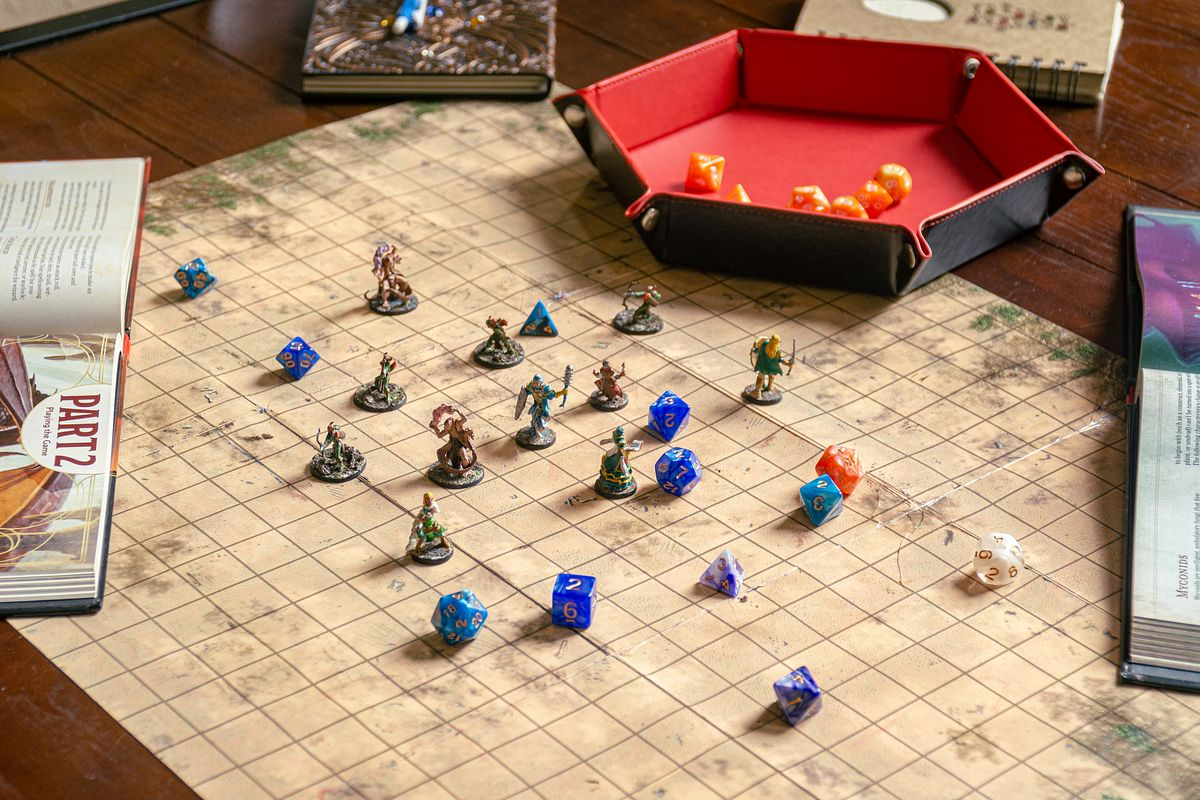
\includegraphics[width=0.45\textwidth]{Imagenes/Bitmap/dndsencillo}%
\end{SubFloat}
\qquad
\begin{SubFloat}
{\label{fig:dnddiorama}%
	Imagen de un diorama para el escenario de una partida de D\&D, extraída de \cite{dnddioramaimg}.}%
	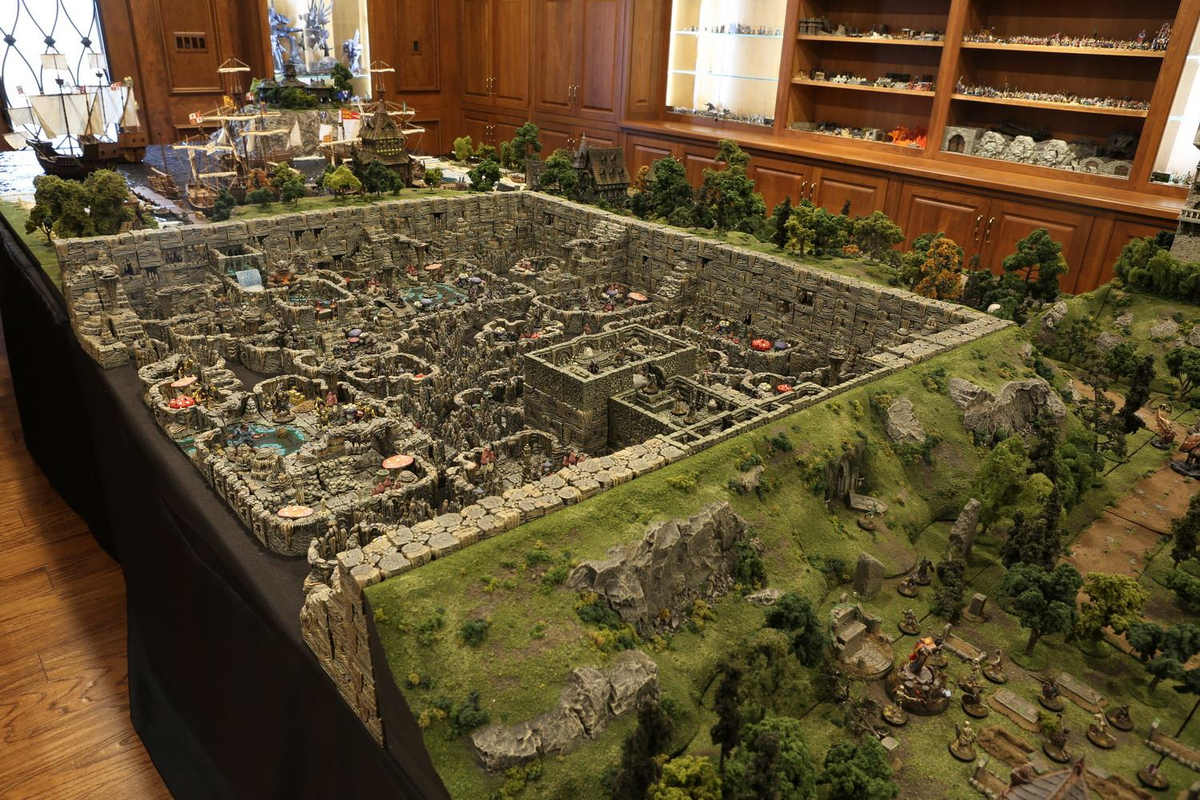
\includegraphics[width=0.45\textwidth]{Imagenes/Bitmap/dnddiorama}%
\end{SubFloat}
\caption{Imágenes de distintas variedades de partidas de \textit{Dungeons \& Dragons}. \label{fig:dndejemplos}}
\end{figure}

Como se ha mencionado anteriormente, \cite{ogdnd}, a veces conocido únicamente como D\&D, es ampliamente conocido como el primer juego de rol comercial y el más influyente del género, y su origen se basa en el sistema de reglas de \cite{chainmail}, al cual se le añadieron elementos de exploración, personajes individuales y narrativa.

\medskip

D\&D se estructura en torno al concepto de un grupo de aventureros que exploran mundos de fantasía, enfrentan criaturas, resuelven conflictos y evolucionan mediante un sistema de niveles y experiencia. El director de juego (aquí llamado \textit{dungeon master}, DM) narra la historia, describe el mundo y controla a los NPC y eventos.

\smallskip

A partir de la tercera edición, del año 2000, se introduce el \textit{sistema d20}, un dado de veinte caras en el que se basa todo el sistema de reglas, así como hojas de personaje detalladas con diversos atributos.

\medskip

En la figura \ref{fig:dndejemplos} podemos ver varios ejemplos de partidas de D\&D, siendo la que está capturada en la figura \ref{fig:dndsencillo} un ejemplo de una partida normal, con un tablero y sus diferentes \textit{d20}, y, en la figura, \ref{fig:dnddiorama}, un ejemplo de un diorama creado por un aficionado a la maquetación, que cuenta con todo lujo de detalles y que llega a ocupar toda una sala.

\medskip

El juego ha pasado por múltiples ediciones, cada una introduciendo cambios en las mecánicas, balance y filosofía de diseño. Su edición más reciente, la quinta, del año 2014, ha tenido un gran éxito comercial y ha contribuido al resurgimiento del juego de rol gracias a su gran accesibilidad, su enfoque narrativo y la visibilidad en plataformas como YouTube o Twitch.

\medskip

El impacto de este juego en la cultura popular y en el diseño de otros juegos es difícil de sobreestimar, ya que está considerado el estándar de facto en los TTRPG y ha inspirado hasta adaptaciones cinematográficas\footnote{La saga \textit{Dungeons \& Dragons} \citep{dndpeli} ha recaudado más de 250 millones de dólares en total sumando las cuatro películas, siendo la última entrega, de 2023, la más exitosa de todas.}.

\subsection{\textit{Pathfinder}}
\cite{pathfinder} nació como una evolución del \textit{sistema d20} de D\&D. Ante el cambio de enfoque que supuso la cuarta edición de D\&D, muchos jugadores buscaron una alternativa que conservara la complejidad y flexibilidad del sistema anterior. Se aprovechó de la licencia OGL (\textit{Open Game License}, Licencia de Juego Abierto)\footnote{Esta licencia se usa principalmente en TTRPG y concede, por parte de los diseñadores, permisos de modificación, copia y redistribución de algunos de los contenidos diseñados para sus juegos, principalmente mecánicas.} para crear un sistema propio que mejorara y expandiera el marco de reglas original.

\medskip

El juego destaca por su nivel de detalle, la personalización de personajes y la riqueza de opciones tácticas durante el combate. El sistema de creación de personajes permite una gran variedad de combinaciones de clases, habilidades, dotes y objetos mágicos. Esto atrae especialmente a jugadores que valoran la optimización mecánica y la profundidad estratégica.

\medskip

Narrativamente, matiene el enfoque épico y de alta fantasía de D\&D, pero con mundos propios, combinando elementos clásicos con tramas políticas, horror cósmico o mitologías exóticas.

\smallskip

En 2019 se publicó su segunda edición, que renovó el sistema con nuevas mecánicas más modernas, como un sistema de tres acciones por turno y una progresión más clara. Pese a que no ha alcanzado el nivel de popularidad de D\&D, \textit{Pathfinder} ha consolidado una gran comunidad y ha mantenido una identidad propia, por lo que muchas páginas lo sitúan siempre en segundo o tercer lugar de popularidad\footnote{La página \textit{The Dragon's Trove} lo sitúa en tercer lugar en su histórico: \url{https://www.dragonstrove.com/blogs/news/the-best-tabletop-rpgs-of-all-time}.}.

\subsection{\textit{Call of Cthulhu}}
\cite{cthulhu} está basado en los mitos creados por H.P. Lovecraft, y representa un enfoque radicalmente distinto al de otros juegos de rol de la época, ya que se centra en la investigación, el horror psicológico y la fragilidad humana ante lo desconocido.

\medskip

El sistema utiliza como base las reglas BRP {\textit{Basic Role-Playing}, Juego de Rol Básico}, que utiliza porcentajes para determinar el éxito de las acciones. Los personajes son investigadores en los años 20 (aunque hay adaptaciones a otras épocas), y deben enfrentarse a cultos secretos, criaturas indescriptibles y horrores cósmicos. A diferencia de otros juegos, la muerte o locura de los personajes es común y está integrada en la narrativa, lo que fomenta una experiencia inmersiva y tensa.

\medskip

El atributo de cordura (SAN, del inglés \textit{sanity}) es central, ya que los encuentros con lo sobrenatural pueden erosionar la mente de los personajes hasta conducirlos a la locura. Esta mecánica refleja la atmósfera opresiva de las obras \textit{lovecraftianas} y crea un estilo de juego más introspectivo y sombrío.

\medskip

\textit{Call of Cthulhu} ha sido aclamado por su capacidad de generar tensión narrativa, y ha influido en muchos otros juegos de rol e investigación, convirtiéndolo en un pilar fundamental del rol narrativo.

\subsection{\textit{Warhammer Fantasy Roleplay}}
\figura{Bitmap/warhammer}{width=0.9\textwidth}{fig:warhammer}{Partida de \textit{Warhammer Fantasy Battle}, extraída de \cite{warhammerimg}.}

\cite{warhammer} comparte ambientación con el universo de miniaturas de \cite{warhammerbattle} (ver figura \ref{fig:warhammer}), pero se diferencia por su tono más oscuro, realista y decadente.

\medskip

Ambientado en un mundo inspirado en la Europa del Renacimiento, pero plagado de corrupción, magia caótica y criaturas monstruosas, WFRP pone al jugador en la piel de personajes que suelen comenzar como personas comunes (rateros, campesinos o aprendices), y no como héroes épicos. El juego enfatiza la progresión lenta, la supervivencia y la toma de decisiones difíciles.

\medskip

Su sistema de reglas, basado también en porcentajes, incluye un sistema de carreras profesionales que estructura el desarrollo del personaje de forma naturalista. Las heridas son graves, la corrupción mágica puede deformar al personaje, y la muerte puede llegar de forma repentina. Esto genera un entorno de juego más peligroso y centrado en la narrativa emergente.

\medskip

WFRP es un referente del estilo conocido como \textit{grimdark}\footnote{La expresión \textit{grimdark} proviene de una de las entregas de la saga \textit{Warhammer}, concretamente, \textit{Warhammer 40000}, en la que se explica que \comillas{In the \textbf{grim dark}ness of the far future there is only war} (En la sombría oscuridad del futuro lejano solo hay guerra).}, que enfatiza mundos crueles, moralidades grises y destinos trágicos. Esta saga ha sido particularmente influyente en Europa, y ha servido de inspiración para sagas de videojuegos como la de \textit{The Witcher}.
\chapter{Videojuegos de Rol}
\label{cap:videojuegosrol}

\begin{resumen}
En este capítulo se explicará qué son los videojuegos, haciendo un enfoque en los videojuegos de rol, se introducirá su historia y se hablará del proceso de desarrollo de estos, analizando la importancia de los motores y editores en el desarrollo de videojuegos.
\end{resumen}

\section{¿Qué es un videojuego?}
Definir qué es un videojuego es una tarea bastante complicada, sobre todo teniendo en cuenta los matices con los que se puede definir (académicos, de diseño, experimentales o tecnológicos). Una de las definiciones más acertadas la da \cite{EspositoVJ}, que lo define como \comillas{un \textit{juego} que se \textit{juega} gracias a un \textit{aparato audiovisual}, y que puede estar basado en una \textit{historia}}. El propio \citeauthor{EspositoVJ} se encarga de definir qué es el \textit{juego}, qué es \textit{jugar}, qué es el \textit{aparato audiovisual} y qué es la \textit{historia}.

\smallskip

La diferencia fundamental de los juegos tradicionales frente a los videojuegos es la existencia de ese \textit{aparato audiovisual} (videoconsolas, ordenador, dispositivos móviles) que pueda ofrecer una interacción \comillas{humano-máquina}, ya que es esta interacción recíproca la que hace que los videojuegos sean videojuegos y no otro tipo de entretenimiento multimedia.

\medskip

A la hora de diseñar un videojuego, hay que tener en cuenta tres conceptos importantes, dos de ellos propuestos por \cite{mda} en su modelo MDA\footnote{El modelo MDA de \citeauthor{mda} intenta cerrar las posibles brechas entre el diseño y el desarrollo de un juego basándose en tres aspectos fundamentales: mecánicas, dinámicas y estética (\textit{\textbf{M}echanics-\textbf{D}ynamics-\textbf{A}esthetics}).}, las mecánicas, las dinámicas y la jugabilidad:
\begin{itemize}
	\item Las \textbf{mecánicas} son las reglas, sistemas y acciones posibles dentro del juego. Incluyen elementos como el movimiento, la recolección de objetos, el combate o el sistema de progresión de los personajes. Se podrían definir como \comillas{los bloques de construcción del juego}.
	\item Las \textbf{dinámicas} son los comportamientos emergentes que surgen de la interacción entre el jugador y las mecánicas, y están estrechamente relacionadas con la experiencia del jugador. Por ejemplo, una mecánica de sigilo puede generar una dinámica de tensión y precaución.
	\item La \textbf{jugabilidad} (o \textit{gameplay}) es la experiencia interactiva del jugador dentro de un videojuego. Pese a que ni \cite{tekinbas2003rules} ni \cite{schell2019art} dan una definición concreta, hablan de cómo la interacción entre el jugador con las reglas del juego y con las mecánicas (es decir, las dinámicas) dan lugar a la jugabilidad. No solo cada juego tiene una jugabilidad distinta que depende de las dinámicas, mecánicas y reglas, sino que puede haber una mecánica emergente que surja a través de las decisiones que cada jugador tome.
\end{itemize}

\medskip

Dependiendo de las mecánicas principales, los objetivos y las formas de interacción que tenga un videojuego, se pueden clasificar en una amplia variedad de géneros.

\smallskip

Los primeros intentos de clasificar los videojuegos mediante características comunes surgen en la década de los 80, principalmente por diseñadores y desarrolladores, como \cite{Crawford84}, quien los categorizó entre aquellos que \textit{requieren de habilidades previas por parte del usuario} (como juegos de combate o de carreras), y \textit{juegos de estrategia} (que engloba al resto de juegos, como los de aventuras, los educativos, y los RPG). Estas categorías son \textit{funcionales}, se centran en las mecánicas de juego y enfatizan cómo los jugadores interactúan con el sistema.

\medskip

Esta categorización ha ido cambiando a lo largo de la historia, hasta llegar a la actualidad, donde los distintos géneros vienen dados por una mezcla de mecánicas, temas, elementos narrativos, estética o lugar de origen y plataforma, y están gravemente influenciados por las tendencias del mercado, discursos mediáticos y la propia percepción de los jugadores. También, muchas veces se quiere categorizar a los videojuegos con etiquetas propias de otras modalidades, como el cine o la literatura, que son incapaces de capturar los aspectos únicos que definen a un videojuego.

\smallskip

Entre esta categorización más \comillas{clásica} se encuentran los siguientes géneros:
\begin{itemize}
	\item Acción, que son todos aquellos juegos que se centran en la velocidad de reacción del jugador y en la coordinación, como por ejemplo juegos de disparos (\textit{shooters}) o plataformas.
	\item Aventura, que prioriza la exploración, la narrativa y, a veces, la resolución de acertijos, como en los juegos \textit{point-and-click}.
	\item Estrategia, que requieren una planificación táctica, ya sea en tiempo real (RTS, \textit{real-time strategy}) o por turnos (TBS, \textit{turn-based strategy})
	\item Simulación, que buscan reproducir aspectos de la vida real, como la gestión de recursos, la conducción de un vehículo o pilotaje de un avión.
	\item Deportes y carreras, que emulan disciplinas deportivas o competiciones de velocidad.
	\item Puzles, que plantean desafíos cognitivos lógicos o espaciales.
	\item Rol, que atendiendo a la definición dada en el capítulo \ref{cap:juegosrol}, son todos aquellos juegos que permitan a sus usuarios encarnar el rol de uno o varios personajes en un mundo ficticio, donde puedan tomar decisiones, interactuar con su entorno y desarrollar una narrativa para conseguir un determinado objetivo.
\end{itemize}

\medskip

\figura{Bitmap/botw}{width=0.7\textwidth}{fig:botw}{Escena de juego de \cite{BOTW}, extraída de \cite{BOTWForbes}.}

\cite{FailGeneros} argumentan que las categorías existentes a día de hoy se quedan cortas para satisfacer los propósitos del género en videojuegos (identidad, agrupación, \textit{marketing} y educación), ya que dada la gran diversidad de juegos que hay ahora, resulta casi imposible poder agrupar la naturaleza multifacética de estos en etiquetas tan \comillas{tradicionales}.

\smallskip

El ejemplo más claro se ve en uno de los juegos más exitosos de la última década, \citegame{The Legend of Zelda: Breath of the Wild}{BOTW}, que mezcla elementos de libre exploración (lo que lo convertiría en un \textit{sandbox} o \comillas{juego libre}), como bien se puede apreciar en la figura \ref{fig:botw} por el enorme mundo en el que se desarrolla la acción; acción en tiempo real e investigación y resolución de rompecabezas (lo que lo convertiría en un juego de \comillas{acción-aventura}); y la progresión en tiempo real del personaje característica de los RPG (se puede ir consiguiendo nuevas habilidades o mejorando el equipamiento). Es por eso que muchas veces hay géneros intermedios, como en este caso, que se podría considerar a \textit{Breath of the Wild} como un RPG de acción (ARPG, \textit{action role-playing game}), que igualmente siguen sin englobar a la increíble diversidad de juegos. Este problema también se puede aplicar a la inversa, donde juegos como \citegame{Undertale}{Undertale}, esencialmente un RPG, tiene elementos, como el combate, propios de otro género de juegos.

\medskip

Hay muchas formas de evitar este problema, y quizá la mejor solución sea dejar de considerar a los géneros como \comillas{cajones estancos} en los que un videojuego no pueda pertenecer a dos de estas categorías simultáneamente \citep{Apperley}, sino que sean más bien un espectro, sin fronteras establecidas, en el que un videojuego pueda caer entre dos categorías distintas.

\smallskip

En resumen, antes de categorizar un videojuego en según qué género, hay que entender que resulta imposible que este se reduzca a una fórmula fija, sino que hay que entenderlo como una combinación fluida de mecánicas, elementos narrativos, temas y estética, que varían de juego a juego.

\subsection{Historia de los videojuegos de rol}

\figura{Bitmap/dnd1975}{width=0.6\textwidth}{fig:dnd1975}{Interfaz de \cite{dnd}, extraída de \cite{dndimage}.}

Es a mediados de la década de los 70 cuando se puede hablar del nacimiento de los videojuegos de rol. Dadas las limitaciones tecnológicas de la época, los RPG primitivos no eran más que simples adaptaciones de juegos de mesa ya existentes por entonces, como \citegame{dnd}{dnd}, una adaptación del anteriormente mencionado \textit{Dungeons \& Dragons}, de donde se tomó su sistema de combate e historia; y posteriormente, en juegos más modernos, se ha tomado el \textit{sistema d20}, las estadísticas de los personajes, o los sistemas de niveles. 

\smallskip

Estos primeros juegos contaban con interfaces basadas en texto, resaltadas con colores muy vivos, y pocos \textit{sprites}, muchas veces llegando a dibujarlos utilizando caracteres ASCII (ver figura \ref{fig:dnd1975}), y normalmente estaban programados en los grandes ordenadores que se encontraban en campus universitarios como los de Harvard o la Universidad de Illinois. Esta primera etapa, \cite{barton2008dungeons} la denomina como la etapa de \comillas{años oscuros}\footnote{En un símil con los años oscuros del Medievo europeo, ya que es un período caracterizado por la falta de literatura e historia escritas y por una decadencia constructiva y cultural.}, ya que es escasa la información que hay hoy en día sobre estos juegos, autores o desarrollo, ya que muchos no se han conservado y se consideran \textit{lost media}, es decir, materiales multimedia que ya no existen en ningún formato y para los cuales no hay ninguna copia disponible.

\smallskip

\begin{figure}[t]
\centering
\begin{SubFloat}
{\label{fig:rogue}%
	Captura de \cite{rogue}, extraída de \cite{rogueimg}}%
	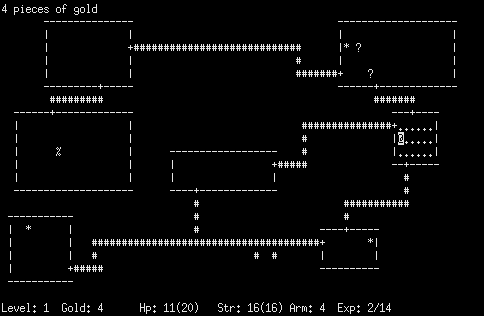
\includegraphics[width=0.45\textwidth]{Imagenes/Bitmap/rogue}%
\end{SubFloat}
\qquad
\begin{SubFloat}
{\label{fig:ultima}%
	Captura de \cite{ultima}, extraída de \cite{ultimaimg}}%
	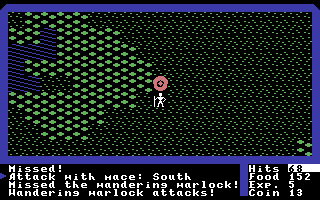
\includegraphics[width=0.45\textwidth]{Imagenes/Bitmap/ultima}%
\end{SubFloat}
\caption{Capturas de \textit{Rogue} y \textit{Ultima}. \label{fig:rogueultima}}
\end{figure}

De esta primera etapa también cabe mencionar tres videojuegos que dieron comienzo a tres distintos subgéneros dentro de los RPG: 
\begin{itemize}
\item \citegame{Rogue}{rogue}, que dio lugar a los videojuegos de mazmorra o \textit{roguelikes}, caracterizados por la generación aleatoria de un laberinto o mazmorra (ver figura \ref{fig:rogue}) en el que se desarrolla una aventura basada en turnos. En este tipo de juegos la muerte es permanente, y al perder la partida se empieza en una nueva desde cero. 
\item \citegame{Wizardry}{wizardry}, que dio lugar a los videojuegos de exploración de mazmorra o \textit{dungeon crawlers}, similares a los anteriores, pero centrados en la exploración de la mazmorra, con un énfasis en la progresión de los personajes y de la gestión de la \textit{party} o escuadrón (el conjunto de personajes que juntos intentan alcanzar objetivos comunes). 
\item \citegame{Ultima}{ultima}, que dio lugar a los RPG de mundo abierto. En esta clase de juegos, los jugadores pueden explorar libremente ciudades, mazmorras, bosques y otro tipo de entornos, manteniendo las mecánicas tradicionales de otros RPG (ver figura \ref{fig:ultima}). 
\end{itemize}

\medskip

Con el salto tecnológico que hubo a mediados de la década de los 80, los RPG comienzan a separase cada vez más de ser meras adaptaciones de juegos ya existentes a desarrollar sus propias historias. A partir de esta época se pueden encontrar dos corrientes bastante diferenciadas de RPG, los \comillas{occidentales} (WRPG, \textit{Western role-playing game}), con más libertad de decisión para los jugadores tanto en personalización como en la historia, y con temáticas realistas (como los anteriormente mencionados \textit{Rogue}, \textit{Wizardry} y \textit{Ultima}); y los \comillas{orientales} o \comillas{japoneses} (JRPG, \textit{Japanese role-playing game}, por ser Japón el país que más videojuegos de este tipo produce), centrados en una narrativa lineal con temáticas fantásticas y mecánicas basadas en turnos. Dos grandes videojuegos que definieron el género de los JRPG son \citegame{Dragon Quest}{dq} y \citegame{Final Fantasy}{ff}, cuyas sagas permanecen hasta la actualidad con nuevas entregas cada pocos años. Son estos años de apogeo de los RPG los que \citeauthor{barton2008dungeons} denomina como \comillas{etapa dorada}.

\medskip

La década de los 90 supuso un grave declive para los RPG \comillas{occidentales}, ya que la aparición de juegos de acción en 3D, como \citegame{Doom}{doom}, \citegame{Quake}{quake} o \citegame{Tomb Raider}{lc}, hizo que el mercado cambiase hacia este tipo de juegos, mucho más rápidos y frenéticos que los RPG, que se consideraban obsoletos, con una pesada carga textual y mucho más lentos de jugar. También, la aparición de videoconsolas mucho más potentes y baratas, como la \textit{PlayStation} (Sony, 1994) o la \textit{Nintendo 64} (Nintendo, 1996), para las cuales estos RPG no tenían portabilidad\footnote{Son muchas las decisiones por las cuales las empresas \comillas{occidentales} no quisieron portar sus juegos hacia las nuevas consolas, como por ejemplo las limitaciones que iba a suponer (algunos requerían teclado y ratón), los altos costes que conllevaba el rediseño de muchos de los juegos y la poca demanda que se consideraba que los juegos iban a tener en estas plataformas.}, y los altos costes de desarrollo y producción que supuso el cambio de cartuchos tradicionales a nuevos formatos como CD-ROM, hicieron que los WRPG tuviesen este gran declive que solo pudo recuperarse a mediados de la siguiente década.

\medskip

Este declive, sin embargo no afectó a los JRPG, ya que estos vivieron una etapa de auge y consolidación, especialmente gracias al éxito de las consolas mencionadas y a una fuerte apuesta por el mercado internacional. Sagas como \textit{Final Fantasy} lograron gran reconocimiento global, en especial, con su séptima entrega, \cite{ffvii}, que supuso un punto de inflexión gracias a su espectacular apartado gráfico para la época y a su narrativa cinematográfica. 

\smallskip

Otro fenómeno destacado fue la aparición de la saga \cite{pokemon}, que redefinió el género al introducir mecánicas de colección y combate por turnos simplificado, orientado a un público mucho más joven, pero sin perder la profundidad estratégica. Otros títulos como \cite{chronotrigger}, \cite{secretofmana}, o \cite{suikoden} aportaron innovaciones tanto en jugabilidad como en narrativa. Gracias a esta explosión de creatividad y accesibilidad, los JRPG no solo sobrevivieron al cambio de tendencias de la industria, sino que se convirtieron en uno de los géneros más representativos de las consolas de 16 y 32 bits.

\medskip

En el nuevo milenio, que para \citeauthor{barton2008dungeons} es la \comillas{etapa de platino}, surgen sagas con juegos con gráficos mucho más sofisticados y con narrativas mucho más profundas, como la saga \textit{The Elder Scrolls}, más concretamente, su tercera entrega, \citegame{Morrowind}{tes}; la saga \citegame{Fallout}{fallout}; la saga \citegame{Baldur's Gate}{baldurs}; o la saga \citegame{Diablo}{diablo}, que llevan hasta el límite las propias definiciones del género por las mezclas con otros géneros (llegando a ser juegos \comillas{híbridos}). La potencia del \textit{hardware} va en aumento, lo que permite que haya un salto cualitativo, tanto gráfico como en jugabilidad, mientras que la tendencia de los mundos abiertos continúa y se mejora, llegando a ser algunos RPG como \citegame{The Elder Scrolls V: Skyrim}{skyrim} o \citegame{The Witcher 3: Wild Hunt}{witcher} los más vendidos\footnote{Según la revista \textit{TheGamer}, en un artículo del año 2021 (\url{https://www.thegamer.com/highest-selling-rpgs-all-time/}), sitúan a \textit{The Witcher 3} como el cuarto juego más vendido con treinta millones de copias, al igual que a \textit{The Elder Scrolls V}, que se sitúa en segundo lugar con las mismas ventas.}.

\section{Sobre el desarrollo de videojuegos}
Para entender cómo, bien las empresas profesionales o bien equipos \textit{indies} desarrollan un videojuego desde cero, es imprescindible saber con exactitud cómo funciona el software internamente, y qué formas tienen los programadores o desarrolladores para comunicarse con las entrañas de este durante el proceso de desarrollo. Es por eso que en este apartado se explicará qué es un \textit{motor} y qué es un \textit{editor}.

\subsection{Roles en el desarrollo de videojuegos}
El desarrollo de un videojuego es una tarea multidisciplinar que requiere la colaboración de múltiples individuos expertos en múltiples áreas. Por lo general, los roles más comunes dentro de un equipo de desarrollo profesional\footnote{En proyectos pequeños o empresas \textit{indies} estas funciones pueden solaparse, ya que no siempre se puede contar con expertos en todas las materias.} son los siguientes:
\begin{itemize}
	\item \textbf{Diseñador}: es el responsable de definir las mecánicas del juego, las reglas, los objetivos, la progresión y la experiencia general del jugador. También se encarga del diseño de los niveles, de los sistemas de juego o del equilibrio de la dificultad.
	\item \textbf{Programador}: se encarga de implementar técnicamente el videojuego utilizando lenguajes de programación y motores de desarrollo. Es común que haya programadores especializados en distintas áreas, como la inteligencia artificial, gráficos, físicas o red.
	\item \textbf{Artista}: se encarga de diseñar los elementos visuales del juego, como personajes, escenarios, animaciones y efectos visuales. Dependiendo del estilo del juego, puede haber artistas 2D, 3D, conceptuales ({\textit{concept artist}}) o de interfaces.
	\item \textbf{Diseñador de sonido}: se encarga del diseño y producción de los efectos de sonido, música y ambiente del juego. A menudo colabora con compositores y actores de voz para dotar de identidad sonora al juego.
	\item \textbf{Guionista}: se encarga de crear la historia, los diálogos, el trasfondo y el desarrollo narrativo del juego. Es fundamental en aquellos géneros donde la narrativa tiene un peso importante, como es el caso de algunos RPG.
	\item \textbf{Probador}: su misión es detectar errores, evaluar la jugabilidad y asegurar que el producto final funcione correctamente. Esta fase se conoce comúnmente como QA (\textit{quality assurance}, aseguramiento de la calidad), y es esencial para garantizar una buena experiencia de usuario.
	\item \textbf{Productor}: se encarga de coordinar al equipo, gestionar los tiempos, recursos y comunicación entre los distintos departamentos. Es el vínculo entre el equipo creativo y las partes interesadas externas (como clientes, editoras o inversores).
	\item \textbf{Director creativo}: supervisa la visión general del juego y asegura que todos los elementos (jugabilidad, arte, narrativa...) estén alineados con el concepto original.
\end{itemize}

\subsection{Motor de videojuegos}
\cite{gregory2018game} define un motor de videojuegos (\textit{game engine}) como \comillas{todo aquel \textit{software} extensible que, sin apenas modificaciones, puedan servir de base o cimiento para múltiples videojuegos distintos}. Este \textit{software} es todo el conjunto de herramientas que hacen que por detrás funcione un juego, como por ejemplo, todas las herramientas que se encarguen del \textit{renderizado} o dibujado en pantalla, bien sea en 2D o en 3D, aquellas que se encarguen de la simulación física y detección de colisiones con el entorno, las que se encarguen del sonido, las del \textit{scripting}, animaciones, inteligencia artificial\ldots A todas estas herramientas también se les denomina \textit{motores} (por ejemplo, \textit{motor de render}, \textit{motor de físicas}\ldots).

\smallskip

Estos \textit{motores de tecnología} conforman la infraestructura básica técnica del motor más complejo que las usa, y se usan para abstraer la interacción con el \textit{hardware} o sistema operativo; por lo que un motor de videojuegos también podría describirse como \comillas{una capa de abstracción y herramientas orientadas al desarrollo de videojuegos elaborada sobre \textit{motores de tecnología}}.

\medskip

Debido a las limitaciones tecnológicas de los años 70 y principios de los 80, los primeros juegos se desarrollaban todos desde cero, sin apenas compartir código un juego con otro, ya que cada uno necesitaba una lógica optimizada de una determinada manera que otros no necesitaban o no podían utilizar. Además, los juegos solían ser lanzados para una única plataforma, ya que portar un juego a otra distinta con otra serie de requisitos y limitaciones implicaba reescribirlo desde cero, y muchas veces los desarrolladores eran equipos muy pequeños (llegando a ser incluso de una única persona) y no todas las grandes empresas disponían de departamentos de portabilidad.

\smallskip

No es hasta mediados y finales de la década de los 80 cuando los desarrolladores comienzan a reutilizar código entre juegos y surgen los primeros ejemplos de lo que hoy se podría llamar \comillas{motor}. Uno de los primeros fue el que Shigeru Miyamoto desarrolló en Nintendo para la \textit{Nintendo Entertainment System} (según explica \cite{williams2017history}), que se utilizaría en juegos como \citegame{Excitebike}{excitebike} o \citegame{Super Mario Bros.}{smb}.

\smallskip

A principios de los 90 surgen los primeros \comillas{motores modernos}, de la mano de desarrolladoras como \textit{id Software} y juegos como \textit{Doom} o \textit{Quake}, quienes decidieron reutilizar toda la lógica de \textit{renderizado} y los sistemas de simulación física, ya que cada parte estaba desarrollada de manera independiente. Tal fue el éxito que alcanzaron estos dos juegos que muchas empresas prefirieron pagar a \textit{id Software} por una licencia del núcleo del motor y diseñar sus propios recursos, que desarrollar su propio motor desde cero. Una de estas empresas fue \textit{Valve}, quienes desarrollaron uno de los mejores juegos de la historia, \citegame{Half-Life}{hl}, utilizando el motor \textit{GoldSrc} (que es el antecesor del actual motor de Valve, \textit{Source}), una versión modificada del motor de \textit{id Software}.

\medskip

Con la generalización de internet a principios de los 2000, comenzó el auge de comunidades de \textit{modding} en línea, y muchas desarrolladoras comenzaron a lanzar motores de código abierto acompañados por editores de niveles o herramientas de \textit{scripting} (es decir, código de alto nivel, normalmente no compilado, que solo modifica lógica del juego o eventos sin modificar el núcleo del motor).

\smallskip

A día de hoy, las empresas dedican numerosos recursos a la hora de desarrollar nuevos motores, ya que son la parte fundamental del desarrollo de videojuegos, y cada vez son más sofisticados y requieren de un gran conocimiento en programación o en diseño.

\smallskip

Los desarrolladores \textit{indie}, por su parte, tienen la posibilidad de poder desarrollar sus propios motores, cuyo contenido no es equiparable al de empresas que producen juegos \textit{triple A} (aquellos juegos producidos por grandes empresas a los que se suelen destinar un alto presupuesto en desarrollo y publicidad); usar motores propietarios de empresas con licencias gratuitas o de poco coste, como por ejemplo \textit{Unity} o \textit{Unreal Engine}; o motores de código abierto, como \textit{Godot}. Por lo general, estos motores suelen venir acompañados de un editor, que facilita el desarrollo de los juegos implementados para ese motor.

\subsubsection{Componentes de un motor de videojuegos}
\begin{figure}[t]
	\begin{center}
		\begin{tikzpicture}[enginebox/.style={draw, thick, minimum width=9cm, minimum height=6cm, align=center},
  subbox/.style={draw, thick, minimum width=3.8cm, minimum height=1cm, align=center},
  labelbox/.style={draw, thick, minimum width=3cm, minimum height=1cm, align=center}]
  			\node[labelbox] (game) {\textbf{Juego}};
	
			\node[enginebox, below=1.5cm of game] (engine) {\textbf{Motor}};
	
			\node[subbox, anchor=north west] at ([xshift=0.5cm, yshift=-0.3cm]engine.north west) (render) {Motor de \textit{render}};
	
			\node[subbox, right=0.5cm of render] (physics) {Motor de físicas};
	
			\node[subbox, below=0.3cm of render] (sound) {Motor de sonido};
	
			\node[subbox, right=0.5cm of sound] (input) {Motor de \textit{input}};
	
			\node[subbox, below=2.1cm of render] (net) {Motor de red};
	
			\node[subbox, right=0.5cm of net] (scripting) {Motor de \textit{scripting}};
	
			\node[subbox, below=0.3cm of net] (anim) {Sistema de animación};
	
			\node[subbox, right=0.5cm of anim] (AI) {Motor de IA};
	
			\draw[->, thick] (game.south) -- node[midway, right] {utiliza} (engine.north);
		\end{tikzpicture}
		\caption{Representación esquemática de la estructura de un juego y su motor con algunos de los componentes principales} 
		\label{fig:juegoymotor}
	\end{center}
\end{figure}

Cada motor de videojuegos es distinto, y cada uno incorpora según qué motores de tecnología dependiendo de las necesidades de los programadores o del juego que se esté programando. Siguiendo el esquema provisto en la figura \ref{fig:juegoymotor}, estos son los componentes principales de un motor de videojuegos tanto de grandes empresas, como motores con licencia gratuita, como aquellos de código abierto:
\begin{itemize}
\item \textbf{Motor de render o de dibujado}: se encarga de gestionar todas las tareas relacionadas con los gráficos que se muestran en pantalla. Para ello, dibuja objetos bidimensionales o tridimensionales, representados generalmente mediante \comillas{mallas}, a través de técnicas de informática gráfica, como pueden ser la \textit{rasterización} o el trazado de rayos. También es el encargado de gestionar la cámara, luces, sombras, materiales y texturas, y puede aplicar diversos efectos de posprocesado al fotograma final. Muchas de estas tareas las puede definir el propio programador haciendo uso de un tipo de \textit{script} especial llamado \textit{shader}, que en lugar de ejecutarse en el procesador de un ordenador se ejecuta en el procesador de las tarjetas gráficas. Estos motores suelen ser una capa de abstracción sobre especificaciones estándar para gráficos como \textit{OpenGL}, \textit{Vulkan}, \textit{DirectX} o \textit{Metal}.
\item \textbf{Motor de físicas}: se encarga de simular comportamientos físicos realistas. Entre estos comportamientos físicos se encuentran las colisiones de objetos con otros objetos o con el entorno, aplicar la fuerza de gravedad a unos determinados objetos, simular las dinámicas de cuerpos rígidos (es decir, el movimiento de cuerpos interconectados bajo la acción de una fuerza externa, como por ejemplo, cajas que se pueden tirar, deslizar o romper), simular dinámicas de cuerpos blandos (similares a los cuerpos rígidos, pero con la posibilidad de que estos se deformen), y, en algunos casos, simulaciones de fluidos y de materiales textiles. Ya que hacer una simulación física es complicado, se suelen utilizar motores de terceros, como por ejemplo \textit{NVIDIA PhysX}, \textit{Havok}, \textit{Bullet} o \textit{Box2D}.
\item \textbf{Motor de sonido}: se encarga de gestionar los efectos de sonido, la música, el audio espacial o posicional en dos o tres dimensiones, y todos los efectos sonoros que se pueden aplicar al sonido (reverberación, eco, tono, barrido, mezclado de pistas, oclusión sonora, efecto Doppler, etc\ldots). Algunas librerías utilizadas son \textit{FMOD}, \textit{OpenAL}, \textit{Wwise} o \textit{irrKlang}.
\item \textbf{Motor de \textit{input} o de gestión de la entrada}: se encarga de capturar y procesar eventos de entrada (\textit{input}) del usuario a través de los diversos dispositivos para los que se programe (teclado y ratón, mandos o controladores y pantallas táctiles) y asociarlos a las acciones definidas en el juego.
\item \textbf{Sistema de animación}: gestiona animaciones de \textit{sprites} (los elementos gráficos bidimensionales básicos que representan visualmente objetos dentro del juego) o de esqueletos (\textit{rigging}, usados para personajes tridimensionales). Suelen tener soporte para árboles de mezcla y cinemática inversa.
\item \textbf{Motor de \textit{scripting}}: permite escribir lógica específica del juego utilizando lenguajes de programación de alto nivel (como por ejemplo JavaScript, Lua, C\# o Python), separando la implementación de la jugabilidad de la implementación del motor. El \textit{scripting} se suele hacer mediante lenguajes de programación interpretados y no compilados, por lo que los cambios más pequeños no requieren volver a iterar por todo el proceso de compilado del motor o del juego.
\item \textbf{Motor de red}: se encarga de gestionar el soporte multijugador, es decir, la comunicación y sincronización cliente-servidor o cliente-cliente. El motor de red también incluye sistemas de emparejamiento (\textit{matchmaking}) y de predicción o interpolación del juego para una simulación fluida en los juegos multijugador.
\item \textbf{Motor de inteligencia artificial}: ofrece herramientas para poder crear comportamientos inteligentes artificiales, como por ejemplo, algoritmos de búsqueda de caminos (\textit{pathfinding}, como los algoritmos \textit{A*} o el de Dijkstra), árboles de comportamiento y máquinas de estado, o sistemas de toma de decisiones. Este motor suele tener una conexión directa con el motor de \textit{scripting} para poder definir comportamientos mucho más fácilmente.
\item \textbf{Gestor de recursos}: maneja la carga y descarga de recursos como texturas, mallas, sonidos o animaciones, muchas veces bajo demanda del juego mediante gestores de memoria, compresión y de transmisión de datos altamente optimizados.
\item \textbf{Sistema de interfaz de usuario}: se encarga de gestionar la barra de estado (HUD, \textit{head-up display}), los menús, texto, botones y otros elementos de la interfaz con los que el usuario pueda interactuar.
\end{itemize}

\subsubsection{Separación entre motor y \textit{gameplay}}
\begin{figure}[t]
\centering
\begin{SubFloat}
	{\label{fig:separaciongeneral}%
		Separación en motores generalistas.}%
		\begin{tikzpicture}
		\draw (0,0) rectangle (3,6);
		\draw[red, dashed] (-1,2) -- (4, 2);
		\node at (1.5,4) {\textit{Gameplay}};
		\node at (1.5,1) {Motor};
		\end{tikzpicture}
\end{SubFloat}
\qquad
\begin{SubFloat}
	{\label{fig:separacionespecificos}%
		Separación en motores específicos.}%
		\begin{tikzpicture}
		\draw (0,0) rectangle (3,6);
		\draw[red, dashed] (-1,4) -- (4,4);
		\node at (1.5, 5) {\textit{Gameplay}};
		\node at (1.5, 2) {Motor};
		\end{tikzpicture}
\end{SubFloat}
\caption{Ejemplos de separaciones entre motor y \textit{gameplay} en los distintos motores. \label{fig:separacionesmotgp}}
\end{figure}

Para poder reusar un motor en múltiples juegos con el menor número de cambios, es necesario saber \textit{cómo y para qué vamos a desarrollar el motor}, y de acuerdo a la decisión que se haya tomado, se establecerá la barrera de separación entre el motor y la jugabilidad del juego.

\medskip

Los motores más generalistas, como los anteriormente mencionados \textit{Unity}, \textit{Unreal Engine} o \textit{Godot}, debido a que están pensados para poder ejecutar todo tipo de juegos, tienen una barrera de separación entre el motor y el \textit{gameplay} que se suele establecer a la mitad. La implementación del juego final que tienen este tipo de motores es mínima (el motor es puramente un conjunto de \textit{motores de tecnología}) y es el desarrollador, o a veces el diseñador\footnote{En muchos casos, hay veces que los propios diseñadores también pueden implementar parte del juego sin la necesidad de tener conocimientos de programación. Para ello, existen los editores, que se explicarán en la sección \ref{sec:editorvj}.}, el que se tiene que encargar del desarrollo de la jugabilidad. En la figura \ref{fig:separaciongeneral} se puede ver esta \comillas{separación} de manera esquemática, donde la parte de la jugabilidad es mucho más amplia que la del motor, que solo incluye elementos básicos para que un juego funcione. 

\smallskip

La gran ventaja que tienen los motores generalistas frente a los específicos es la libertad que dejan al desarrollador (o diseñador) para poder implementar la jugabilidad a su manera, con las reglas y mecánicas que se hayan establecido previamente.

\medskip

En el caso de aquellos motores que fijan gran parte de la jugabilidad de los juegos que se puedan hacer con ellos, y que lo único modificable son algunos parámetros del \textit{gameplay} y las partes artísticas y visuales, se tendrán que introducir elementos propios del juego en el motor, dejando menos libertad de implementación en el \textit{gameplay}. En la figura \ref{fig:separacionespecificos} se aprecia cómo la barrera de separación entre la implementación del juego que contiene el motor frente a la de la jugabilidad es mucho más alta que en la figura \ref{fig:separaciongeneral}, por lo que el motor ya no solo incluirá elementos básicos para el funcionamiento del juego, sino elementos específicos de un tipo de juego en concreto.

\smallskip

Este tipo de motores son mucho más rígidos a la hora de poder implementar nuevas funcionalidades y limitan bastante los juegos que se pueden crear con ellos, pero simplifican bastante el desarrollo, y son especialmente útiles para nuevos programadores.

\subsubsection{Programación dirigida por datos (DDP) en videojuegos}
\label{sec:ddp}
La programación dirigida por datos (DDP, \textit{data-driven programming}) es un paradigma de diseño en el que gran parte del comportamiento y lógica de un programa están controlados por datos externos en lugar de estar programados en el código fuente de este. Este paradigma, según \citeauthor{gregory2018game}, ampliamente extendido entre las empresas desarrolladoras de juegos \textit{triple A}, permite a los desarrolladores modificar o expandir el comportamiento del juego sin la necesidad de alterar el motor o el código base de este.

\medskip

Los motores de videojuegos suelen estar programados utilizando lenguajes de \textit{medio nivel}\footnote{Los lenguajes de \textit{medio nivel}, como C o C++, son aquellos lenguajes de alto nivel que proporcionan estructuras de acceso a \textit{hardware} propias de los lenguajes de bajo nivel.}, ya que se espera poder optimizar al máximo el programa, así como poder tener un soporte multiplataforma. De todo el gran abanico de lenguajes de nivel medio, un gran porcentaje son lenguajes compilados, es decir, requieren de un \comillas{traductor} (compilador) para generar el código máquina antes de poder ejecutar el programa. Esta compilación depende del tamaño del proyecto y del número de ficheros a compilar, y, en el caso de muchos motores, la compilación puede llegar a tardar decenas de minutos.

\smallskip

Para evitar tener que esperar estos minutos recompilando todo un juego en caso de cambiar un simple parámetro referente al \textit{gameplay}, se opta por la solución más flexible, que es desarrollar todo el juego utilizando datos, generalmente en lenguajes de \textit{scripting}, de alto nivel, como Lua, que no necesitan ser compilados, sino interpretados (la \comillas{traducción} a lenguaje máquina se realiza en ejecución del programa y a medida que sea necesaria) por el motor del juego.

\medskip

Además de reducir los tiempos de compilación en los juegos, lo cual ayuda a reducir los tiempos en las iteraciones de desarrollo, la programación dirigida por datos permite, tanto a desarrolladores como a diseñadores, modificar comportamientos, ajustar parámetros o añadir contenido utilizando archivos de configuración o mediante herramientas visuales.

\medskip

Este paradigma refuerza la ya mencionada separación entre motor y \textit{gameplay}, ya que un mismo motor puede ejecutar distintos juegos (es decir, distintos datos) sin la necesidad de tener que ser recompilado, siempre y cuando los datos estén en un formato y estructura que el motor sea capaz de interpretar.

\medskip

Los datos se suelen almacenar utilizando lenguajes de definición de datos (DDL, \textit{data definition language}), que permiten describir la estructura y organización de estos que el motor o el sistema de \textit{scripting} van a usar. Estos lenguajes, como JSON, XML o incluso formatos binarios diseñados específicamente, que permiten mantener una clara separación entre la lógica del juego y los contenidos, facilitando, a su vez, la escalabilidad del proyecto.

\medskip

Aunque DDP se asocia al uso de motores de videojuegos, su implementación no depende estrictamente de estos. De hecho, es perfectamente posible aplicar DDP sin utilizar un motor formal, siempre que exista una arquitectura que permita interpretar y ejecutar los datos de forma dinámica. Muchos desarrolladores independientes o juegos clásicos sin motor como tal ya hacían uso de este enfoque mediante archivos de configuración, tablas o \textit{scripts} embebidos.

\medskip

Un ejemplo histórico de DDP puede encontrarse en el motor \textit{SCUMM} (\textit{Script Creation Utility for Maniac Mansion}), desarrollado por Lucasfilm Games en los años 80 para facilitar el desarrollo de su aventura gráfica \cite{maniacmansion}. Este motor permitía definir el comportamiento de escenas y personajes mediante \textit{scripts} externos, lo que habilitaba la creación de aventuras gráficas sin necesidad de reescribir el código base. Posteriormente, el motor \textit{GrimE} (\textit{Grim Engine}), también desarrollado por LucasArts\footnote{Lucasfilm Games cambiaría su nombre a LucasArts en 1990, y, posteriormente, en 2021, lo volvería a cambiar por Lucasfilm Games.} y utilizado en juegos como \cite{grimfandango}, amplió este enfoque incorporando Lua como lenguaje de \textit{scripting}, mostrando una evolución clara hacia un diseño aún más flexible y dirigido por datos.

\subsubsection{Programación multiplataforma en videojuegos}
\begin{figure}[t]
	\begin{center}
		\begin{tikzpicture}[
    font=\sffamily,
    platform/.style={rectangle, draw=black, fill=blue!10, minimum width=2.5cm, minimum height=1cm},
    layer/.style={rectangle, draw=black, fill=orange!20, minimum width=10cm, minimum height=1cm},
    core/.style={rectangle, draw=black, fill=green!20, minimum width=10cm, minimum height=1.5cm},
    commonlayer/.style={rectangle, draw=black, fill=magenta!20, minimum width=10cm, minimum height=0.7cm},
    arrow/.style={->, thick}
]

\node[platform] (pc) at (-4, 4) {Motor de PC};
\node[platform] (ps) at (0, 4) {Motor de PlayStation};
\node[platform] (xb) at (4, 4) {Motor de Xbox};

\node[commonlayer] (abstr) at (0, 2.5) {Interfaz común};

\node[core] (engine) at (0, 1.25) {Componentes multiplataforma del motor};

\node[layer] (game) at (0, -1) {Juego};

\node[draw, thick, rounded corners, inner sep=10pt, fit=(pc) (ps) (xb) (abstr) (engine), label=left:{Motor}] (motor) {};

% Arrows
\draw[arrow] (pc.south) -- ([xshift=.-4cm]abstr.north);
\draw[arrow] (ps.south) -- (abstr.north);
\draw[arrow] (xb.south) -- ([xshift=4cm]abstr.north);
\draw[arrow] (game.north) -- ([xshift=-0.1cm]motor.south);

		\end{tikzpicture}
		\caption{Representación esquemática de la arquitectura de un motor multiplataforma} 
		\label{fig:motormultiplat}
	\end{center}
\end{figure}

La programación multiplataforma es una práctica esencial en el desarrollo de videojuegos modernos. Esta característica permite que un mismo juego funcione idénticamente en distintos dispositivos y sistemas operativos (por ejemplo, en el caso de los videojuegos, que funcione en ordenadores Windows, Linux o Mac; en consolas, como PlayStation, Xbox o Nintendo Switch; o en dispositivos móviles, como Android o iOS). Pese a que aumenta las labores de desarrollo del motor (ya que en muchos casos hay que desarrollar módulos específicos para cada una de las plataformas, principalmente de \textit{renderizado}), reduce los costes de mantener un juego y maximiza el alcance de este.

\medskip

Para lograr que un motor sea multiplataforma, hay que tener en cuenta para qué plataformas se va a desarrollar y qué diferencias hay entre cada una de ellas. Es por ello que se suelen utilizar capas de abstracción, que permiten que el núcleo del motor permanezca intacto entre las distintas implementaciones, mientras que son aquellos módulos que difieren de un sistema a otro los que se modifican.

\smallskip

Otro factor a tener en cuenta es la compilación cruzada, es decir, el proceso por el cual el código se compila en una plataforma (principalmente un ordenador con Windows o Linux), pero el ejecutable se genera para una plataforma distinta (por ejemplo, para Android o para PlayStation). Para ello, se deben disponer de herramientas que faciliten la configuración de estas compilaciones.

\medskip

Los principales desafíos en la programación multiplataforma de videojuegos son debidos a las diferencias entre las distintas API (\textit{application programming interface}, interfaz de programación de aplicaciones, es decir, todo el código que permite a dos aplicaciones comunicarse entre sí) de las videoconsolas, tanto en el \textit{render}, como en el manejo de archivos; o las compatibilidades que una librería pueda tener en un sistema o en otro.

\medskip

En la figura \ref{fig:motormultiplat} se puede apreciar el esquema de una arquitectura multiplataforma: por una parte, los nodos azules corresponden a las implementaciones de los \textit{motores de tecnología}, cada una distinta dependiendo de los requerimientos de cada una de las plataformas; el nodo rosa correspondería a la interfaz común de cada uno de los \textit{motores de tecnología}\footnote{Es decir, tanto el motor como el juego deben poder llamar a funciones y clases que estén implementadas de distinta forma en cada uno de los \textit{motores de tecnología} y poder cambiar de plataforma sin que haya ningún error. Para ello se define esta interfaz, que contendrá las definiciones de los nombres pero no su implementación.}; el nodo verde corresponde a toda aquella parte del motor que no depende de ninguna plataforma; y finalmente, el nodo naranja es el juego, que utiliza todo el conjunto del motor para poder funcionar.

\subsection{Editor de videojuegos} \label{sec:editorvj}
\figura{Bitmap/unreal}{width=0.9\textwidth}{fig:unreal}{Vista de la interfaz de \textit{Unreal Engine} 5.2, extraída de \cite{unrealinterfaz}.}

Un editor de videojuegos es una herramienta, generalmente visual, que permite crear, modificar y probar contenido de un juego sin la necesidad de programar directamente en código. Un editor también es especialmente útil para \textit{no programadores}, es decir, diseñadores o artistas que pueden estar involucrados en el desarrollo del juego sin necesariamente tener que saber programar.

\medskip

Por lo general, los editores como el de \textit{Unreal Engine} permiten al usuario diseñar y editar los niveles, mapas o escenarios sobre los que se desarrolla la acción; editar entidades o actores, como personajes, enemigos o NPC; editar \textit{scripts} o crear eventos que definan el comportamiento o la jugabilidad; gestionar y editar recursos como materiales, texturas, partículas o animaciones; y poder ejecutar y depurar una versión del juego para probar y solucionar problemas sin la necesidad de generar un ejecutable final.

\smallskip

\figura{Bitmap/godot}{width=0.8\textwidth}{fig:godot}{Vista del \textit{scripting} visual mediante nodos de \textit{Godot}, extraída de \cite{godotnodos}.}

Una característica esencial de los editores es un sistema de \comillas{hacer-deshacer-rehacer}, que permite a los desarrolladores experimentar con cambios sin riesgo a perder el progreso.

\medskip

En el editor de \textit{Unreal Engine}, mostrado en la figura \ref{fig:unreal}, apreciamos varias de estas características, como la edición de materiales y texturas (cada una de las esferas que se muestran en el cajón inferior representa un material o textura que se puede aplicar a los objetos en la escena), un visor de las entidades que se encuentran en la escena (en la parte derecha, que permite la edición individual de cada una de las entidades, bien sean parte del escenario o personajes y la propia escena (o \textit{viewport}, en grande, en el centro del editor, en la cual el usuario puede mover libremente la cámara y mover, rotar y escalar cada objeto).

\medskip

El editor se aprovecha de los principios de la programación dirigida por datos (ver apartado \ref{sec:ddp}), haciendo posible que los cambios realizados por el usuario se reflejen en el juego sin la necesidad de recompilar el motor ni generando un ejecutable externo. Esto permite poder ejecutar el juego directamente desde el propio editor (\textit{Unreal Engine} lo denomina \textit{Play In Editor}), lo cual agiliza las iteraciones durante el desarrollo.

\medskip

Es importante destacar que el editor no es el motor del juego en sí, aunque está estrechamente ligado a él y hace uso directo de muchas de sus funcionalidades. Mientras que el motor es el componente responsable de ejecutar el juego, el editor actúa como una capa de interfaz que permite manipular los datos que el motor utiliza. Por ejemplo, al colocar un objeto en una escena desde el editor, lo que realmente ocurre es que se modifica un conjunto de datos que el motor luego interpretará en tiempo de ejecución.

\medskip

Algunos editores modernos suelen ofrecer herramientas de \textit{scripting} visual, como es el caso de los \textit{blueprints} en \textit{Unreal Engine} o el sistema de nodos en \textit{Godot} (ver figura \ref{fig:godot}), que permiten implementar la lógica sin tener que escribir código tradicional. Estas herramientas, junto con el patrón ECS (\textit{entity-component-system}, entidad-componente-sistema), una importación automatizada de los recursos, y el poder extender la funcionalidad del editor mediante \textit{plugins} (complementos o extensiones), convierten a los editores modernos en los ejes centrales del flujo de trabajo en el desarrollo de videojuegos.

\subsubsection{Editores específicos de videojuegos para desarrollo de RPG}
\begin{figure}[h]
\centering
\begin{SubFloat}
{\label{fig:rpgmakermz}%
	Vista de la interfaz de \cite{rpgmakermz}.}%
	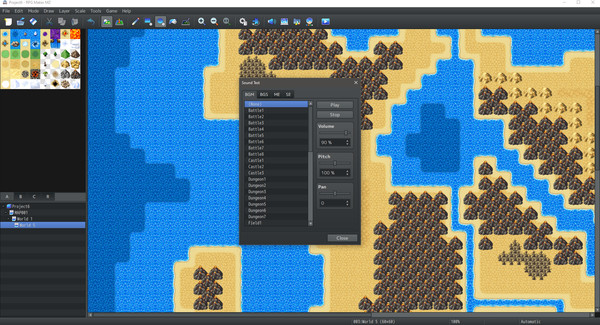
\includegraphics[width=0.45\textwidth]{Imagenes/Bitmap/rpgmakermz}%
\end{SubFloat}
\qquad
\begin{SubFloat}
{\label{fig:rpgmakerevent}%
	Vista del editor de eventos de \textit{RPG Maker MV}, extraída de \cite{rpgmakerevent}.}%
	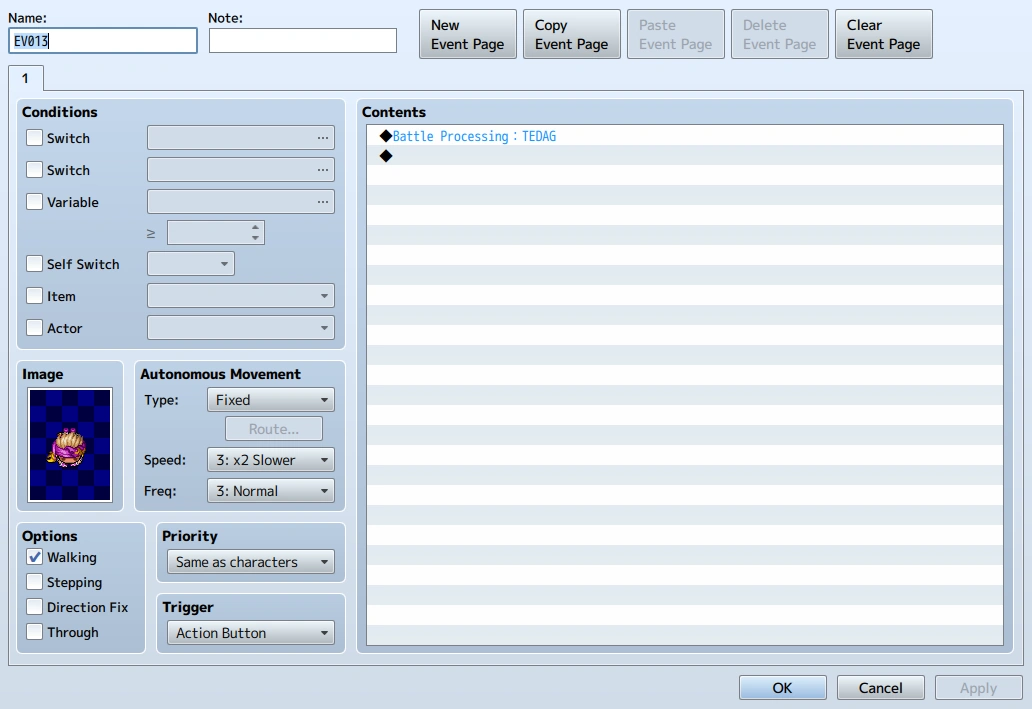
\includegraphics[width=0.45\textwidth]{Imagenes/Bitmap/rpgmakereventeditor}%
\end{SubFloat}
\caption{Capturas de distintos elementos de la interfaz de \textit{RPG Maker}. \label{fig:rpgmaker}}
\end{figure}

Si bien es cierto que una gran parte de los juegos más jugados a diario son RPG\footnote{Según la página \textit{SteamDB}, y, a día 21 de mayo de 2025, un 34\% de los juegos jugados a diario, solamente en PC, son RPG (\url{https://steamdb.info/stats/globaltopsellers/?displayOnly=Game&tagid=122}).}, hay muy pocos motores y editores específicos para este tipo de juegos, y se tiende a usar motores más generalistas. De entre los específicos, necesariamente tenemos que mencionar a la serie de herramientas más conocida de todas, \cite{rpgmaker}\footnote{Según \textit{itch.io}, \textit{RPG Maker} se sitúa como la octava herramienta más utilizada, siendo la primera específica de RPG que aparece en el listado, con más de diez mil proyectos creados a día 21 de mayo de 2025 y subidos a su web (\url{https://itch.io/game-development/engines/most-projects}).}. Se trata de un entorno de desarrollo completo, que combina un motor de ejecución con un editor visual, pensado para permitir a usuarios sin conocimientos avanzados de programación crear juegos completos mediante una interfaz sencilla (ver figura \ref{fig:rpgmakermz}).

\smallskip

El editor incluye un sistema de creación de mapas basado en baldosas, un generador de personajes y una base de datos para poder definir los enemigos, objetos, habilidades, clases, estados y eventos mediante lógica visual (figura \ref{fig:rpgmakerevent}). 

\medskip

Este sistema de eventos es una de las características más potentes y distintivas de \textit{RPG Maker}, ya que permite definir la lógica utilizando una lista secuencial de comandos que representan \textit{acciones}\footnote{Las acciones son instrucciones específicas dentro de un sistema de eventos. Estas acciones son \comillas{bloques} con instrucciones básicas que se ejecutan secuencialmente para definir la lógica del juego, como por ejemplo, \textit{mostrar diálogo}, \textit{mover personaje} o \textit{cambiar una variable}.} y que puede ser utilizado por usuarios sin experiencia alguna, así como otros más curtidos en la materia que pueden crear sistemas más complejos.

\medskip

También se incluye un sistema de batallas tradicional, en el cual los combatientes se van turnando, inspirado en los JRPG clásicos, aunque es posible modificarlo utilizando \textit{plugins} o \textit{scripts} (desarrollados en las últimas versiones en JavaScript), así como la posibilidad de poder exportar los juegos a múltiples plataformas (desde las últimas versiones), como PC, web y dispositivos móviles.

\medskip

El editor de \textit{RPG Maker} permite definir todos estos elementos mencionados anteriormente de forma visual, mientras que el motor es el que se encarga de ejecutar el resultado final. Ambos están estrechamente integrados, permitiendo una experiencia fluida durante el desarrollo, sin la necesidad de recurrir a herramientas externas ni a complejos procesos de compilación.

\bigskip

Además de \textit{RPG Maker}, existen varias alternativas de código abierto, como \cite{rpgpapermaker}, que permite crear RPG en 3D con estética retro. Otras opciones, como \cite{rpgjs} permiten desarrollar los juegos utilizando lenguajes como TypeScript o HTML5 para navegadores\footnote{\url{https://docs.rpgjs.dev/guide/get-started.html}.}.

\smallskip

También encontramos proyectos de código abierto como \textit{EasyRPG}, que busca recrear los contenidos de \textit{RPG Maker 2000/2003} de manera gratuita, facilitando la ejecución de RPG antiguos que ya no tienen soporte en plataformas modernas así como la creación de nuevos juegos sin la necesidad de utilizar un software propietario; o \cite{ohrrpgce} (conocido como OHRRPGCE), que permite crear juegos al estilo de los primeros juegos de la saga \textit{Final Fantasy}\footnote{\url{https://rpg.hamsterrepublic.com/ohrrpgce/About}.}.

\medskip

Por último, se ha elaborado una tabla comparativa entre los distintos \textit{softwares} anteriormente mencionados con algunas de sus características más importantes.

\rotatebox{270}{
\begin{minipage}{\textheight}
\begin{center}
\begin{tabularx}{\textwidth}{@{} l | X | X | X | X | X @{}}
\toprule
\textbf{Característica} & \textbf{RPG Maker} & \textbf{RPG Paper Maker} & \textbf{RPG JS} & \textbf{EasyRPG} & \textbf{OHRRPGCE} \\
\midrule
\textbf{Licencia} & Comercial & Gratuita & Código abierto & Código abierto & Código abierto \\
\addlinespace[4pt]
\textbf{Plataformas} & PC, Web, Móvil & PC, Web & Web & PC, Android, Web & PC, Android \\
\addlinespace[4pt]
\textbf{Gráficos} & 2D & 3D retro & 2D & 2D clásico & 2D clásico \\
\addlinespace[4pt]
\textbf{\textit{Scripting}} & JavaScript (MV/MZ) & JavaScript & TypeScript y HTML5  & Ninguno (eventos visuales) & HamsterSpeak \\
\addlinespace[4pt]
\textbf{Facilidad de uso} & Muy fácil & Fácil & Compleja & Muy fácil & Media \\
\addlinespace[4pt]
\textbf{Personalización}  & \textit{Plugins}/\textit{Scripts} & \textit{Scripts}  & Código fuente & \textit{Scripts} & \textit{Scripts} \\
\addlinespace[4pt]
\textbf{Desarrollo activo} & Sí & Sí & Parcial & Sí & Sí \\
\addlinespace[4pt]
\textbf{Sistema de combate} & Personalizable & Personalizable & Por programar & Por turnos & Por turnos \\
\bottomrule
\end{tabularx}
\end{center}
\end{minipage}
}
\chapter{Planteamiento del Proyecto}
\label{cap:planteamiento}

\begin{resumen}
En este capítulo se tratarán los objetivos principales del proyecto, así como las decisiones tomadas en cuanto a diseño del motor y del editor.
\end{resumen}

\section{Objetivos principales del Proyecto}
La idea principal es el desarrollo de un motor de videojuegos, enfocado a los RPG 2D, acompañado de un editor que permita un desarrollo rápido y simple de juegos de este tipo para el motor desarrollado. El editor está pensado principalmente para gente no programadora o sin experiencia en el desarrollo de videojuegos, por lo que la interfaz tiene que ser intuitiva y fácil de utilizar y aprender.

\smallskip

El editor debe ser capaz de generar un ejecutable, que por debajo utilice el motor desarrollado previamente, con el diseño de juego realizado por el usuario en el propio editor, y que pueda ejecutarse en Windows, MacOS, Linux y Android. El editor, por su parte, ha de poder ser ejecutado tanto en Windows, MacOS o Linux, descartando la ejecución en dispositivos móviles\footnote{Los editores suelen tener elementos que son preferibles de ser utilizados mediante entrada de teclado y ratón. Si bien es cierto que Android permite la conexión de periféricos de entrada-salida, es una plataforma pensada para dispositivos móviles y táctiles.}.

\smallskip

El usuario podrá elegir la plataforma para la cual se va a generar el ejecutable, y el editor se encargará de transferir el contenido desarrollado en el proyecto a la \textit{build}, asegurándose de que el comportamiento volcado es el mismo que el diseñado previamente y generando una \textit{build} lista para empaquetar y distribuir, sin requerir pasos adicionales por parte del usuario.

\medskip

Por otra parte, se espera que el editor pueda generar diversos proyectos (es decir, distintos juegos), y sea capaz de guardar el estado de un proyecto y recuperarlo cuando el usuario desee, sin que se hayan perdido los cambios que se hayan realizado. Y, también, debe poder exportar proyectos, así como importarlos incluyendo aquellos que otros usuarios puedan haber diseñado en otras plataformas o sistemas sin mayor dificultad.

\medskip

El motor, por su parte, aportará la mayor parte del \textit{gameplay}, para que el usuario solo tenga que desarrollar la parte de diseño (principalmente el diseño artístico y visual. Tendrá que tener las funcionalidades básicas que se esperan de un RPG, así como soporte para periféricos de entrada salida tradicionales (teclado y ratón) y entrada táctil (para los dispositivos móviles). 

\section{Toma de decisiones}
\label{sec:decisiones}
La primera decisión a tomar fue la plataforma de desarrollo del Proyecto. Se decidió desarrollar el grueso del Proyecto en C++, ya que se quería aprovechar el alto rendimiento que ofrece en comparación a otros lenguajes\footnote{El hecho de poder gestionar la memoria utilizada en cualquier momento, así como la ausencia de una máquina virtual intermedia hacen que C++ sea el lenguaje idóneo para proyectos donde el rendimiento es crítico.}, el soporte multiplataforma que tiene la familia C/C++ tanto en dispositivos de sobremesa como en móviles, y el uso de librerías más avanzadas que facilitarían el desarrollo del Proyecto.

\medskip

Debido a la premisa de un desarrollo multiplataforma, se necesitaba usar un IDE (\textit{integrated development environment}, entorno de desarrollo integrado) que fuese compatible tanto con Windows, MacOS, y Linux. La opción que en un principio se había valorado era la de utilizar \textit{Visual Studio}, una de las herramientas más populares para el desarrollo en C++; sin embargo, debido a que este IDE carece de versiones para MacOS y Linux\footnote{MacOS y Linux cuentan con \textit{Visual Studio Code}, que si bien sirve para poder compilar C/C++ mediante el uso de \textit{plug-in}, es más complicado de configurar para proyectos más complejos como este.}, se optó por hacer el desarrollo del Proyecto en \textit{CLion}, un IDE con soporte para CMake, que facilitaría a la hora de agilizar el trabajo (por su rapidez en la generación de proyectos complejos) y con la gestión de las dependencias externas.

\smallskip

Pese a que el aprender a usar CMake ocupó gran parte del inicio del desarrollo del Proyecto, las ventajas que ha supuesto a la hora del manejo de las distintas dependencias externas frente a otras alternativas que se habían manejado a lo largo del transcurso del Grado, han hecho que la inversión temporal en esta opción haya resultado beneficiosa.

\medskip

Por otra parte, para el desarrollo del motor, se tendría que utilizar otra herramienta para el desarrollo de la APK (\textit{Android Application Package}, paquete de aplicaciones Android, es decir, el ejecutable de Android), ya que esta se debe desarrollar utilizando Java. Por esto se decidió utilizar \textit{Android Studio}, la herramienta oficial de desarrollo para Android, que proporciona máquinas virtuales de dispositivos Android de distintas versiones y generaciones para poder probar la \textit{build}. Otra ventaja añadida al uso de Android Studio es el soporte que tiene para CMake, que ha permitido disponer de un único archivo de configuración para ambas herramientas.

\smallskip

Dentro de \textit{Android Studio}, se tiene que añadir también el módulo de NDK (\textit{Native Development Kit}, kit de desarrollo nativo) que permite el desarrollo de aplicaciones para Android utilizando llamadas a C/C++ gracias a JNI (\textit{Java Native Interface}, interfaz nativa de Java) integrada en el SDK de Java. JNI es un ejemplo de una FFI (\textit{foreign function interface}, interfaz de funciones foráneas), es decir, un mecanismo por el cual un lenguaje de programación puede llamar a funciones o rutinas programadas o compiladas en otro lenguaje distinto, lo cual es necesario para poder ejecutar el juego, ya que la entrada de la aplicación Android está en Java.

\medskip

El resto de decisiones son propias de cada una de las partes del Proyecto y se detallarán a continuación.

\subsection{Diseño del motor}
\subsubsection{Base con el sistema entidad-componente}
El objetivo del motor es poder ejecutar juegos RPG, por ello deberá implementar sus sistemas y permitir su uso a alto nivel. Sin embargo, aún teniendo la separación entre motor y \textit{gameplay} de un motor específico en este alto nivel, a bajo nivel estos sistemas estarán construidos alrededor de estructuras modulares propias de motores generalistas.

\medskip  

La base del motor se estructurará atendiendo a un patrón EC (entidad componente) y los sistemas específicos de los juegos RPG se construirán sobre esa base. Lo primero a tener en cuenta en esta parte es el bucle de juego.

\medskip  

En este bucle de juego es en el que se actualizarán los elementos de cada juego. Estos elementos están organizados según una jerarquía. La primera pieza son las escenas. Cada escena se define como un conjunto de entidades. A su vez, cada una de estas entidades es quien representa cualquier elemento del juego: un personaje, un obstáculo, un cuadro de texto... Para definir cuál será el comportamiento de cada una de las entidades estas contienen un conjunto de componentes. Los componentes encapsulan funcionalidades específicas, se pueden crear de múltiples tipos permitiendo una gran flexibilidad a la hora de marcar el funcionamiento de cada entidad. Gracias a esta estructura se podrán implementar una amplia variedad de mecánicas mediante la creación de distintos componentes.  

\medskip

Una vez con esta estructura montada, para funcionar necesita conocer qué escenas, entidades y componentes debe utilizar. Para este propósito se crea un sistema de gestión de recursos. Definimos recurso, o \textit{asset}, como todo aquel elemento externo al código del programa que este usará para obtener el comportamiento deseado, estos pueden ser por ejemplo imágenes, audios, fuentes de texto... La forma en la que este sistema se conecta con el anterior es a través de estos recursos. Cada una de las escenas se definirá en un fichero que el motor interpretará como un recurso con el que crearlas dentro del programa. De esta forma el motor no deberá conocer de antemano estas escenas y su contenido permitiendo un uso mucho más ligero.

\smallskip

Estos recursos de escenas estarán descritos cada uno en un fichero Lua y son lo que definirá el \textit{gameplay} de cada juego. Lua ha sido elegido por su simplicidad, su integración fluida con C++ mediante librerías como \texttt{sol2}, y su compatibilidad multiplataforma. Estas librerías proporcionan \textit{bindings}, es decir, código que facilita el uso de Lua desde C++ y viceversa.

\medskip

Además de la carga de escenas, el sistema de carga de recursos permitirá gestionar múltiples tipos de recursos que pueden ser utilizados por el resto del motor. Cuando se solicite un recurso, este se cargará en memoria si no lo estaba previamente. Esta operación se realizará hasta alcanzar un límite de memoria, definido por el usuario. Una vez alcanzado dicho límite, si se solicitase un nuevo recurso, se aplicará un algoritmo LRU (\textit{least-recently-used}, usado menos recientemente), que liberará el recurso que más tiempo lleve sin usarse para hacer espacio al nuevo.

\subsubsection{Componentes genéricos de juego}
Para desarrollar videojuegos, es necesario contar con ciertas funcionalidades básicas que faciliten la implementación de los sistemas específicos del juego.

\smallskip

En el motor, se utilizará la librería \texttt{SDL3} para implementar estos sistemas. Esta elección se debe principalmente, a su sencillez de uso y a su robusto soporte multiplataforma, que permite ejecutar los juegos tanto en sistemas de escritorio como en dispositivos Android.

\medskip

Los sistemas que se implementarán serán los siguientes:
\begin{itemize}
	\item Sistema de \textit{renderizado}: es imprescindible contar con un mecanismo que permita mostrar visualmente lo que ocurre en el juego. Dado que se trata de un motor para videojuegos 2D, se usarán imágenes y texto para cubrir esta necesidad. Estos sistemas de \textit{renderizado} se expondrán al usuario a través de componentes que permitirán mostrar y animar imágenes, mostrar texto y controlar una cámara desplazable. Además, se implementará un sistema de \textit{renderizado} basado en capas y escenas, que permitirá superponer diferentes escenas, lo cual resulta útil para mostrar elementos (como menús) en forma de \textit{overlay}, y permite tener un mayor control sobre el orden de \textit{renderizado}.
	\item Sistema de entrada: se desarrollará un sistema de \textit{input} sencillo basado en clics y toques. Este diseño garantiza la compatibilidad multiplataforma y permite centrar la jugabilidad en la interacción mediante botones, en línea con la experiencia tipo \textit{point-and-click} que se quiere ofrecer. El motor unificará la entrada mediante clic y toque en una estructura común que incluya la posición del evento y su estado (inicio, mantenido o final) en un determinado fotograma.
	\item Sistema de sonido: la retroalimentación auditiva es un componente esencial en los videojuegos. Para su implementación, se empleará el nuevo sistema de sonido incluido en \texttt{SDL3}. Para lograr este propósito se creará un componente que permita reproducir, pausar, detener y reanudar los sonidos. Además, estos pueden agruparse en diferentes conjuntos, lo que permite controlar de forma independiente el volumen general, el de música y el de los efectos sonoros.
	\item Sistema de colisiones: está diseñado para cubrir las necesidades de los juegos previstos, donde será suficiente con detectar intersecciones entre rectángulos. A través del componente correspondiente, será posible comprobar si un objeto colisiona con otro, si acaba de entrar en colisión o si ha dejado de colisionar.
\end{itemize}

\subsubsection{Componentes específicos de RPG}

Para la navegación por el mundo el motor ofrece un sistema de mapas. Cada mapa será una de las áreas de un juego especificada por el diseñador. Estos mapas están formados por casillas y cada una de ellas puede contener \textit{tiles}. Los \textit{tiles} son imágenes preparadas para combinarse modularmente de forma que en conjunto dibujen un escenario. En estos mapas también se podrán definir los elementos interactivos del juego como, por ejemplo, los NPC.

\medskip  

Sobre estos mapas, se ha diseñado un sistema de movimiento automático y detección de colisiones basado en una cuadrícula de casillas y un algoritmo A* de búsqueda de caminos. Para ello, se mantendrán actualizadas las posiciones ocupadas dentro de la cuadrícula, tanto por elementos estáticos como por elementos dinámicos, y se recalculará la ruta siempre que sea necesario. Este sistema se aplicará tanto a los NPC, a través del sistema de eventos y sus comportamientos asociados, como al jugador, mediante un sistema de entrada de tipo \textit{point-and-click}.

\medskip

También se implementará un sistema de carga dinámica de mapas y transición entre ellos. Mientras el jugador se encuentra en un determinado mapa, el motor cargará en segundo plano los mapas adyacentes. Al cambiar de un mapa a otro, se descargarán aquellos que ya no sean necesarios. Esta estrategia permite equilibrar el uso de memoria y los tiempos de carga, ofreciendo una solución eficiente y escalable.

\medskip

Adicionalmente, se dispondrá de un sistema de diálogos con cuadros de texto que muestren el contenido de forma de dinámica. El jugador podrá avanzar en la conversación mediante una entrada sencilla, mientras que el motor gestionará automáticamente los saltos de línea y el ajuste del tamaño del texto. Asimismo, se integrará un selector de opciones que permita al jugador elegir entre distintas alternativas mediante botones interactivos.

\smallskip

Las decisiones tomadas se registrarán, lo que permitirá diseñar desde el editor sistemas de interacción complejos al estilo clásico de los RPG. Este sistema hará uso de variables locales (propias de cada objeto del mapa) y globales del jugador (asociadas a la partida), permitiendo un control detallado de la progresión sin requerir programación adicional.

\medskip

Por último, se desarrollará un componente destinado a facilitar el diseño de la lógica específica del juego mediante comandos sencillos: el gestor de eventos. Este componente constituirá el núcleo del sistema de interacción y comportamiento en el mundo del juego.

\subsubsection{Sistema de eventos}
Uno de los objetivos principales del motor es ofrecer la posibilidad de crear un RPG sin necesidad de conocimientos de programación. Para ello, se ha diseñado un sistema de eventos: una estructura que permite controlar la lógica del juego mediante instrucciones de alto nivel.

\medskip

La idea fundamental es sencilla: gracias al componente de gestión de eventos, una entidad podrá contener un conjunto de eventos. Dentro del motor se define un evento como una combinación de una condición y una serie de comportamientos.

\medskip

La condición determinará bajo qué circunstancias deberá activarse el evento. Existirán múltiples tipos de estas condiciones de alto nivel, encargadas de evaluar distintos aspectos del estado del juego. Algunas de ellas son, por ejemplo, si el jugador ha interactuado con un elemento o si ha pasado un cierto tiempo desde un instante. Si una condición se cumple su evento asociado comenzará su ejecución. Además, será posible combinar condiciones mediante operadores lógicos (\textit{not}, \textit{or}, \textit{and}), lo que permitirá definir reglas más complejas y flexibles.

\medskip

La segunda parte del evento serán los comportamientos, encargados de definir qué acciones se deben realizar una vez activado el evento. Estos comportamientos actuarán como una lista de instrucciones que modifiquen el estado del juego a través de parámetros sencillos. Estarán escritos en Lua y se encargarán de invocar distintas funciones del motor: desde mover objetos, cambiar animaciones o modificar la música, hasta iniciar diálogos.

\medskip

El sistema está diseñado para que la ejecución de los comportamientos sea progresiva: en cada actualización del juego se ejecutará uno de los comportamientos activos del evento. En los casos en los que una acción requiera más de una actualización para completarse, el comportamiento se limitará a establecer un objetivo, que será procesado por el resto de sistemas mientras el evento continúa ejecutando el resto de sus comportamientos.

\medskip

Existirán además comportamientos orientados al control del flujo de ejecución. Por ejemplo, uno de ellos permitirá esperar a que se cumpla una condición antes de continuar, actuando como un mecanismo de bloqueo temporal. También, se implementarán instrucciones de salto que permitirán la creación de bucles o la bifurcación de la ejecución según el estado del juego.

\medskip

Gracias a este sistema, que actúa como lenguaje de \textit{scrpting} simplificado, será posible crear lógicas de juego complejas mediante herramientas accesibles y visuales, sin la necesidad de escribir código complejo.

\subsection{Diseño del editor}
\figura{Vectorial/editorMapas}{width=\textwidth}{fig:mapeditor}{Editor de mapas de \baker.}

\subsubsection{Funcionalidad del editor}

La esencia del editor es la de una interfaz intuitiva y sencilla de utilizar y aprender para aquellos usuarios noveles que nunca hayan utilizado una herramienta similar. Para evitar cargar cognitivamente a los usuarios con información textual, se ha optado por el uso de símbolos e iconos acompañados por descripciones emergentes cortas en la mayoría de elementos.

\medskip

Las características fundamentales que el editor tiene corresponden con aquellos elementos que pueden ser modificados en el motor, es decir:
\begin{itemize}
	\item Editor de mapas (figura \ref{fig:mapeditor}), que permitiese al usuario cargar sus propios \textit{tilesets}; decidir el tamaño de la cuadrícula que ocuparía el mapa; dibujar el mapa sobre la cuadrícula utilizando las baldosas del \textit{tileset}, con la posibilidad de tener varias capas para poder simular un efecto de profundidad; y establecer las regiones de colisión del mapa.
	\item Editor de eventos, que permitiese al usuario la creación de eventos, asignándoles la condición de lanzamiento y los comportamientos que se ejecutarán cuando la condición se cumpla. El editor de eventos tendría que tener soporte para eventos complejos, en el caso de que el usuario requiera de la creación de uno de ellos.
	\item Editor de \textit{sprites} y de animaciones, que permitiese al usuario generar un \textit{sprite} dada una imagen o \textit{spritesheet}, y, posteriormente, animaciones dada una serie de \textit{sprites}. Ambos editores tendrían una previsualización del \textit{sprite} o animación, añadiéndose controles para la reproducción en este último caso. 
	\item Editor de objetos, que permitiese al usuario generar un objeto para cada una de las baldosas en la cuadrícula del mapa y asignarle un \textit{sprite} y un evento.
	\item Editor de personaje, que permitiese al usuario personalizar su \textit{sprite}, añadirle animaciones de movimiento y configurar diversos parámetros adicionales, como su posición de origen en el mapa.
	\item Editor de conexiones entre los mapas, que permitiese al usuario establecer las posiciones de los distintos mapas en el mundo, de manera visual e intuitiva.
	\item Editor de ajustes generales del ejecutable final, como por ejemplo el nombre del juego, dimensiones de la cámara, la fuente por defecto a utilizar en los textos, o el mapa inicial del juego.
\end{itemize} 

Todos estos elementos tendrían la capacidad de poder ser configurados al gusto del usuario, permitiendo ser editados y eliminados cuando este desee.

\medskip

Además, el editor incluiría un \textit{viewport} para que el usuario pudiese ver en tiempo real el diseño final del juego, sobre el cual se podría ejecutar y probar las funcionalidades implementadas, al estilo de \textit{Unity}.

\medskip

Por otra parte, el editor contará con un sistema de persistencia, que permita una carga y guardado de los \textit{proyectos}, es decir, la representación de un juego en el editor. Todos los \textit{assets} utilizados tendrán que estar referenciados en archivos de configuración del \textit{proyecto}, y el guardado actualizará estos archivos de configuración.

\subsubsection{Modularidad y arquitectura}
En cuanto a la estructura de la interfaz, se optó por utilizar una arquitectura típica en el desarrollo de \textit{software} no relacionado con videojuegos, basado en ventanas (o subventanas) anidadas en otras ventanas, con el uso de ventanas modales que apareciesen sobre estas. Esta estructura permite una escalabilidad del proyecto mucho más sencilla en caso de futuras expansiones y una mayor modularidad con cada uno de los componentes que se quisiese integrar.

\medskip

Las ventanas tendrían comunicación unas con otras utilizando al \textit{proyecto}, que almacenaría toda la información referente a cada uno de los juegos que el usuario crease (por ejemplo, referencias a los \textit{tilesets}, \textit{sprites}, animaciones o mapas creados).

\smallskip

Se tendrían también diversos gestores, tanto de \textit{scripting}, como de elementos de entrada salida de ficheros, como de preferencias del usuario y hasta un gestor de idiomas, que permite que el Proyecto sea multilingüe\footnote{En un principio, únicamente en castellano y en inglés, pero debido al sistema implementado, es muy sencillo añadir nuevos idiomas en el caso que fuese necesario.} con una amplia escalabilidad en el caso de que se quisiesen añadir más idiomas.

\subsubsection{Tecnologías utilizadas}

Para conseguir todos los objetivos anteriores, se investigó qué librerías se iban a poder utilizar para conseguir desarrollar toda la interfaz y la funcionalidad básica. Al ofrecer las facilidades necesarias para los objetivos de esta parte del proyecto, como el soporte multiplataforma, se optó por \texttt{SDL3} como base para el editor, acompañada de \texttt{DearImGui} para el dibujado y manejo de los elementos de la interfaz.

\medskip

También, al ya haber optado por el uso de Lua como lenguaje de \textit{scripting} y de definición de datos para el motor, se optó por el uso del mismo para el editor, acompañados por la anteriormente mencionada librería \texttt{sol2}.

\smallskip

Los archivos de configuración del proyecto difieren de los que el motor espera recibir, ya que muchas veces el editor espera recibir más datos de los que el motor necesita (por ejemplo, rutas específicas de \textit{assets}, guardado de \textit{tilesets}, etc.). Es por eso que el editor se tiene que encargar de \comillas{traducir} estos ficheros de definición de datos a los datos que el motor espera; esto se hará en el tiempo de generación del ejecutable final. Esta decisión se ha tomado para que, si no se dispone de los ficheros de configuración del \textit{proyecto}, un usuario ajeno al diseño del juego sea incapaz de poder modificarlo, al igual que ocurre en la gran mayoría de motores\footnote{Esto es debido a que, en muchos casos, se quiere que el jugador final evite poder hacer modificaciones al juego si no dispone del código original de este, evitando posibles casos de piratería o distribución no autorizada.}.

\medskip

Si bien es cierto que una de las técnicas más comunes en la implementación de un editor es la de utilizar el motor para el que se desarrolla como base, ya que esto evita el tener que implementar dos veces las mismas funcionalidades (principalmente en \textit{renderizado}, \textit{input} y \textit{scripting}), se decidió independizar el desarrollo del editor del motor para poder avanzar más rápidamente en el Proyecto. Esta opción, pese a que ha supuesto una mayor carga de trabajo, ha permitido flujos de iteración en el desarrollo más cortos.

\chapter{Motor}
\label{cap:motor}

El desarrollo del motor se fundamenta en 4 capas, cada una con distintos sistemas y utilidades. 

\section{\textit{Core}}
En primer lugar, la base del \texttt{Core} está formada por un sistema de Entidades y Componentes organizados en escenas, junto con un sistema de carga de recursos que lee tanto archivos fuente como archivos \texttt{.lua}.

\subsection{Sistema de entidad-componente}
El entorno de juego consta de múltiples Componentes, cada uno contenido en una Entidad. Estas Entidades se agrupan en escenas, que gestiona el \texttt{SceneManager}.

\smallskip

La lógica de cada componente se rige por un ciclo de vida con las siguientes fases: 

\begin{itemize}
	\item \texttt{Init}: se invoca solo una vez al crear el componente, durante la construcción de la Entidad o más adelante en tiempo de ejecución. Su función es inicializar atributos, ya sea obteniendo referencias de otros elementos de la escena o leyendo parámetros desde un objeto \texttt{ComponentData} que contiene datos leídos del archivo \texttt{.lua}.
	\item \texttt{Update}: se llama en cada iteración del bucle principal, aquí reside la mayor parte de la lógica del componente. Se puede evitar que esta llamada ocurra desactivando el componente y viceversa mediante un método \texttt{setEnabled(true/false)}.
	\item \texttt{OnEnable / OnDisable}: se disparan al activar o desactivar el componente respectivamente. Además, si un componente comienza habilitado al cargar la escena, \texttt{OnEnable} se invoca automáticamente.
\end{itemize}

\medskip

Cada Entidad mantiene sus Componentes en un diccionario ordenado, donde la clave es un entero que define el orden de ejecución. Además, cada una de ellas puede tener otras Entidades hijas: cada una almacena un conjunto sin ordenar de punteros a sus hijas y un puntero a su padre. La propia Entidad propaga las llamadas de \texttt{Update} y el resto del ciclo de vida a sus hijos, la escena solo conserva referencias a las raíces de la jerarquía. Para eliminar una Entidad, se marca su atributo \texttt{Alive} en \texttt{false} y luego se purga en la llamada a \texttt{refresh} que ocurre tras cada \texttt{Update}.

\medskip

Las escenas guardan sus Entidades raíz en un conjunto sin orden y ejecutan recursivamente las llamadas correspondientes sobre cada rama de la jerarquía. También mantienen un diccionario de \comillas{handlers}, claves únicas de tipo \textit{string}, para referenciar rápidamente Entidades desde cualquier componente. Además, almacenan referencias a los \texttt{RenderComponent} registrados, organizados por capas, que se explicarán más adelante. 

\medskip

Por último, tenemos al \texttt{SceneManager}, quien se encargará de la gestión de escenas, de instanciar nuevos objetos a partir de \textit{blueprints} y de conectar las llamadas del bucle principal con la escena activa. Las escenas en el \texttt{SceneManager} se organizan en una lista que hace las veces de pila: podemos añadir escenas con \texttt{push\_back} y eliminarlas con \texttt{pop\_back}, y la que esté al final (\texttt{back}) es la que se considera activa. Sin embargo, mantenemos la estructura como lista para poder iterar sobre ella durante el renderizado, ya que queremos pintar todas las escenas, no solo la activa.

\medskip

Esta base está preparada para funcionar con múltiples escenas distintas con diferentes entidades y componentes que se carguen desde archivos de datos. Para que esto funcione así, se ha implementado un sistema de gestión de recursos en el motor.

\subsection{Sistema de gestión de recursos}
La segunda parte fundamental de la base del motor es el sistema de gestión de recursos. Su objetivo es poder cargar distintos tipos de recursos de forma genérica y flexible para poder implementar funcionalidades dependientes de archivos externos. Para poder hacerlo este sistema consta de tres partes esenciales: 

\begin{itemize}
	\item \texttt{Resource} es una clase base que sirve como interfaz para poder crear cualquier tipo de recurso que se necesite. Permite implementar dos métodos \texttt{load()} y \texttt{unload()}. El primero es el que se encargará de leer el archivo correspondiente a ese recurso y almacenar su contenido en memoria. El segundo liberará la memoria reservada por el primero invalidando los accesos posteriores que se puedan hacer sobre el recurso. Además de esto, esta clase da acceso a un parámetro en el que cada uno de los recursos registrará el espacio ocupado en memoria. Este podrá ser consultado desde otras partes del código para poder tener una gestión de memoria más profunda.
	\item \texttt{ResourceHandler} es una clase plantilla que sirve para poder acceder a los distintos tipos de recursos que implementen la interfaz \texttt{Resource}. Usa el patrón \textit{singleton}, pues queremos permitir que se pueda acceder a los recursos desde cualquier punto del motor. Su función principal es devolver un recurso que se pueda acceder a partir de un archivo dado. Con su método \texttt{get(key)} se encargará de crear el recurso solicitado en el motor si no lo estaba y retornarlo. 
	\item \texttt{ResourceMemoryManager} se encarga de controlar qué recursos permanecen cargados y cuánto espacio de memoria están ocupando. A través de un archivo de configuración se puede establecer cuál es el límite de memoria que se quiere usar para los recursos; esta clase es la que se encarga de que ese umbral no se supere. A través de un algoritmo LRU se gestiona qué recursos están cargados en cada instante. Cada vez que se quiera usar alguno de estos, es decir, cada vez que se llame a \texttt{get(key)} de un \texttt{ResourceHandler}, se le solicitará a este gestor de memoria que lo active. Esta activación consiste en tres fases. Primero comprobar si el recurso está ya cargado, si es así simplemente se actualizará en el LRU. En caso contrario, iría al segundo paso que es cargarlo y comprobar si hay espacio suficiente, de ser así se almacenaría. Si no, el tercer paso es crear ese espacio y, a través del LRU, se irán descargando aquellos recursos que lleven más tiempo sin ser utilizados, hasta que haya espacio suficiente para que el nuevo se almacene.
\end{itemize}

\medskip

Sobre estas tres piezas fundamentales está estructurado el sistema de gestión de recursos y, adicionalmente, existen otras dos clases que ayudan en esta tarea. \texttt{ResourceManager}, que se encarga de inicializar el sistema con la configuración dada y establecer la conexión entre \texttt{ResourceMemoryManager} y los \texttt{ResourceHandler}. Y \texttt{LuaReader}, que ofrece una interfaz sencilla para poder extraer tablas de Lua guardadas en un archivo o dentro de otra tabla de Lua. La lectura de estos archivos se hace a través de \texttt{SDL}, para poder mantener la funcionalidad entre plataformas, y la interpretación a través de \texttt{sol2}.

\subsection{Carga de escenas a partir de datos}
Una parte fundamental de los motores de videojuegos es que han de permitir ejecuciones con resultados distintos dependiendo de los datos que se le aporten. Esto es para poder reutilizar en videojuegos completamente distintos las herramientas que este ofrece. Se usará un paradigma conocido como programación dirigida por datos, \textit{data-driven programming}. 

\medskip

Las escenas son un conjunto de entidades que se definen en archivos \texttt{.lua}. Estos archivos se leen en tiempo de ejecución y se almacenan en diferentes \textit{blueprints}, que guardan la información esencial para que el motor pueda instanciar escenas, entidades y componentes a partir de ellos. Podemos diferenciar cuatro tipos de \textit{blueprints}: 

\begin{itemize}
	\item \texttt{SceneBlueprint}: se guarda como recurso del sistema de carga. Lee un archivo \texttt{.lua} con el nombre de la escena y almacena todas las entidades definidas en él en un vector de \texttt{EntityBlueprints}. Más adelante, el \texttt{SceneManager} lo utiliza para crear la escena, iterando sobre el vector de entidades e instanciándolas. 
	\item \texttt{EntityBlueprint}: contiene la información necesaria para crear e instanciar una entidad. Normalmente, forma parte de un \texttt{SceneBlueprint}. Guarda todos los hijos como \texttt{EntityBlueprints}, en un vector \texttt{children}, y todos sus componentes en un vector de \texttt{ComponentData}. Adicionalmente, almacena dos variables: el \texttt{handler}, un \textit{string} que, si no está vacío, se registra en la escena para poder referenciar esa entidad; y un \textit{booleano}, \texttt{active}, que indica si la entidad se instancia activa o inactiva en la jerarquía de la escena, esto significa que no recibirá llamadas a \texttt{update} ni a \texttt{render}. El \texttt{SceneManager} recorre recursivamente los hijos llamando al método de creación de entidad y luego itera sobre los componentes para añadirlos e inicializarlos con los parámetros almacenados en cada \texttt{ComponentData}. 
	\item \texttt{PrefabBlueprint}: es una subclase de \texttt{EntityBlueprint} que se guarda como recurso independiente mediante herencia múltiple. Funcionalmente es idéntico, pero en lugar de formar parte de un \texttt{SceneBlueprint}, se lee desde su propio archivo de recurso y se mantiene de forma separada. El \texttt{SceneManager} lo utiliza para instanciar entidades en tiempo de ejecución, por ejemplo, en el sistema de mapas.
	\item \texttt{ComponentData}: almacena toda la información necesaria para crear e inicializar un componente. Consta de dos elementos: 
		\begin{itemize}
			\item El identificador de componente, un \textit{string} que se usa para crear la una instancia de la clase de componente correspondiente. 
			\item \texttt{data}, una tabla de \texttt{sol2} donde se guardan los valores de inicialización de los distintos parámetros. 
		\end{itemize}
\end{itemize}

\medskip

Para crear los componentes a partir de la información de estos \texttt{ComponentData} surge el problema de tener que crear objetos de clases distintas a partir de identificadores. La solución aplicada en este caso es el uso del patrón factoría. En una clase \texttt{ComponentFactory} se registrará la creación de cada tipo de componente asociada a un identificador. Con esto se le podrá solicitar a esta clase crear cada tipo de componente haciéndole llegar un identificador. 

\smallskip

Para poder definir ese identificador fácilmente en cada componente se ha creado un paso intermedio en la herencia de estos, \texttt{ComponentTemplate}. Cada componente derivará de este permitiendo definir el identificador de cada componente fácilmente en su declaración.

\smallskip

Con esto, a partir de un objeto \texttt{ComponentData}, el \texttt{SceneManager} crea los componentes mediante \texttt{ComponentFactory}, estos \textit{blueprints} conservan la tabla \texttt{data} para usarla en su llamada a \texttt{init}. Para evitar el uso directo de los métodos de \texttt{sol2} en cada componente, \texttt{ComponentData} proporciona las interfaces \texttt{getData} y \texttt{getArray}, que permiten obtener los valores almacenados. Además, \texttt{ComponentData} incluye en su propia tabla \texttt{data} un indicador que señala si el componente debe instanciarse habilitado o deshabilitado.

\section{Componentes genéricos de juego}
De cara a facilitar el desarrollo de videojuegos los motores ofrecen implementaciones de sistemas que se usan en la gran mayoría de estos. Hay múltiples bibliotecas que facilitan la adición de estas funcionalidades, en este caso se usará \texttt{SDL3} que ofrece todo lo necesario para desarrollar de forma sencilla lo diseñado además de ofrecer soporte multiplataforma.

\subsection{\texttt{Render}}
Para el apartado de \textit{renderizado} utilizamos las funciones que ofrece \textit{SDL}. El \texttt{RenderManager} se encarga de generalizar estos métodos para que los componentes de \textit{render} puedan acceder a ellos fácilmente. Para ello implementa: 

\begin{itemize}
	\item \texttt{clear}: se llama al comienzo de cada fotograma y vacía el \textit{buffer} de vídeo para preparar el siguiente \textit{renderizado}.
	\item \texttt{present}: se invoca al final de cada fotograma, después de llamar a todos los \texttt{RenderComponent}; muestra el contenido del \textit{buffer} de vídeo en pantalla.
	\item \texttt{drawRect}: rellena un rectángulo de tamaño y posición dados con el color indicado.
	\item \texttt{drawSprite}: dibuja un fragmento de una imagen en la posición de pantalla y con la rotación indicadas.
	\item \texttt{drawText}: dibuja un bloque de texto creada previamente en la posición y rotación indicadas. 
	\item \texttt{setViewRect}: establece el \textit{viewRect}, es decir, el fragmento del mundo que se va a ver en pantalla. Ajusta desplazamientos y reescalados antes de dibujar los elementos.
\end{itemize}

El ciclo de \textit{renderizado} de cada fotograma es: 
\begin{enumerate}
	\item Llamar a \texttt{clear} para limpiar el buffer.
	\item Invocar \texttt{render} en el \texttt{SceneManager}, que lo replica en cada escena y, a su vez, en todos los \texttt{RenderComponent} registrados. 
	\item Llamar a \texttt{present} para mostrar el resultado.
\end{enumerate}

Este proceso se repite durante todo el ciclo de vida de la aplicación.

\medskip

Además, el \texttt{RenderManager} gestiona la inicialización y el cierre de los subsistemas de \textit{SDL} relacionados, así como la creación de la ventana de vídeo.

\medskip

El resto de la funcionalidad de vídeo se concentra en los componentes de \textit{render} (\texttt{RenderComponent}) y en los recursos que utilizan. Implementa el método \texttt{Render(RenderManager*)} en el que realiza las llamadas a los métodos de \textit{renderizado} necesarios. Todos dependen de un \texttt{Transform} que indica posición, rotación y escala, y especifican su capa para organizar el orden de dibujo. Los \texttt{RenderComponent} se registran en la escena en \texttt{OnEnable} y se desregistran en \texttt{OnDisable}, con lo que la escena controla qué componentes están activos en cada momento.  

\medskip

Las llamadas de \textit{renderizado} se realizan en orden inverso de la pila de forma que las escenas que estén más abajo en la pila se llaman primero y por lo tanto se ven por debajo de las siguientes. Además, dentro de cada escena los \texttt{RenderComponent} se llaman en orden de capas de forma que las capas más altas se pintan las últimas.

\medskip

Los \texttt{RenderComponent} implementados son: 

\begin{itemize}
	\item \texttt{Camera}: modifica el área de \textit{renderizado} llamando a \texttt{setViewRect}. Tiene un tamaño lógico en píxeles y su posición se controla mediante su \texttt{Transform}. Por defecto usa la capa \texttt{-1} para que su llamada \texttt{Render} sea la primera de la escena.
	\item \texttt{Rectangle}: guarda tamaño y color, y dibuja un rectángulo en la posición del \texttt{Transform}. 
	\item \texttt{Text}: crea una \texttt{TextTexture} a partir de fuente, tamaño, color, centrado y texto, y la dibuja en la posición del \texttt{Transform}.
	\item \texttt{SpriteRenderer}: dibuja un \texttt{Sprite} (fragmento de textura cargada desde una imagen) en la posición del \texttt{Transform}. 
	\item \texttt{Animator}: subclase de \texttt{SpriteRenderer} que añade funcionalidad de animación mediante \texttt{Animation}. 
\end{itemize}

Las clases auxiliares de recursos son: 

\begin{itemize}
	\item \texttt{Animation}: guarda un vector con los identificadores de \texttt{Sprite} para cada fotograma, un tiempo de duración y si debe reproducirse en bucle. Se crea desde un archivo \texttt{.lua} con esta información. 
	\item \texttt{Sprite}: almacena el identificador de una textura y el rectángulo correspondiente a la zona a dibujar. 
	\item \texttt{Font}: crea y gestiona una \texttt{TTFFont} de \texttt{SDL} a partir de un archivo \texttt{.ttf} y un tamaño. 
	\item \texttt{Texture}: crea y gestiona una \texttt{SDLTexture} a partir de un archivo de imagen. 
	\item \texttt{TextTexture}: genera y administra una textura de texto de \texttt{SDL} a partir de un texto y unas características de fuente.
	\item \texttt{TextureLoader}: \textit{singleton} encargado de crear texturas usando el \textit{renderer} de \texttt{RenderManager}.  
\end{itemize}

Con esta infraestructura podemos dibujar en pantalla todo lo necesario para representar las entidades de nuestros juegos. 

\subsection{Entrada}
El sistema de entrada gestiona toda la información que recogemos de los eventos de ratón y pulsación de \texttt{SDL} en un \texttt{struct} al que podemos acceder desde cualquier lugar del motor mediante un patrón \textit{singleton}. Aunque no se expone directamente la instancia del \texttt{InputManager}, sí es posible obtener una referencia constante al \texttt{struct} que contiene toda la información necesaria para implementar el \textit{gameplay} de los juegos. Decidimos no implementar ningún tipo de entrada por teclado o mando, con el fin de garantizar un diseño multiplataforma sencillo, ya que todas las funcionalidades de \textit{input} que necesitábamos se pueden abstraer con clics o pulsaciones. 

\medskip

En coordinación con este sistema, también creamos el componente \texttt{Button}. Este almacena una \texttt{sol::function} como \textit{callback}, que se invoca con unos parámetros de tipo \texttt{sol::object} cuando detecta un \textit{input} dentro de su área. Gracias a esto, podemos conectar el motor genérico en C++ con la lógica específica de \textit{gameplay} programada en Lua. 

\subsection{Audio}
Este es el sistema que se encarga de controlar la reproducción de sonidos para los juegos. Envuelve al nuevo sistema de sonido de \texttt{SDL3} para ofrecer una interfaz adecuada al resto de sistemas del motor. Está hecho centrando estas funcionalidades alrededor de un componente \texttt{AudioSource}, cuya función es permitir controlar la reproducción de una sola instancia de un sonido. Lo que se busca en \texttt{AudioSource} se puede separar en otras dos clases:

\begin{itemize}
	\item \texttt{AudioClip} se encarga de envolver a \texttt{SDL\_AudioStream} ofreciendo una interfaz simplificada. Representa una pista de sonido, se puede reproducir, pausar, detener o cambiar su volumen entre otros. Almacena un identificador de la pista de audio que representa. Para su funcionamiento se apoya en el sistema de gestión de recursos, con una clase que extiende de \texttt{Resource}, \texttt{AudioClipData}. Cada vez que se quiera hacer una modificación en el estado de la pista se solicitará el acceso al recurso correspondiente a través de su identificador.
	\item \texttt{AudioMixer} simula una simplificación de cómo funciona un mezclador de audio. Puede recibir múltiples entradas de audio y ofrece una salida. Esto significa que, a un \texttt{AudioMixer}, se le pueden conectar tanto múltiples \texttt{AudioClip} como otros \texttt{AudioMixer}. Permite modificar el volumen de reproducción de todos sus elementos conectados. Esto es así para poder permitir un control más preciso de distintos tipos de sonidos. En los videojuegos es típico permitir al jugador controlar tanto el volumen general como el de la música o los efectos de sonido, por ejemplo. De esta manera se pueden estructurar en forma de árbol las distintas salidas de audio para ofrecer esta funcionalidad. Con esto y con una clase \texttt{AudioManager}, encargada de gestionar el dispositivo de salida y las conexiones entre los \texttt{AudioMixer}, se completa la implementación del componente \texttt{AudioSource}.
\end{itemize}

\subsection{Colisiones}
En lo que refiere a detección de colisiones no se busca que el sistema sea especialmente complejo. Los videojuegos que se ofrecerán crear con el motor no necesitan más que comprobaciones sencillas obtenidas a partir de intersecciones entre rectángulos. Para hacer esto el sistema de colisiones consta de dos elementos: 

\begin{itemize}
	\item \texttt{Collider} es el componente que representa un elemento que puede colisionar. Permite la comprobación de si otro \texttt{Collider} acaba de empezar a colisionar, está colisionando o acaba de dejar de colisionar con este. 
	\item \texttt{CollisionManager} es quien se encarga de mantener al día el estado de cada \texttt{Collider}. Cada vez que se crea una instancia del componente se registra en esta clase. En cada actualización de juego se encargará de cambiar los estados en función de las áreas representadas por cada componente. Esto lo hace a través de una sencilla función que proporciona \texttt{SDL} que comprueba si dos rectángulos tienen intersección.
\end{itemize}

\section{Componentes específicos de RPG}
Sobre toda la infraestructura creada en las secciones anteriores se construyen algunos componentes específicos orientados a los juegos RPG que se podrán diseñar en el editor. 

\subsection{Movimiento}
El sistema de movimiento es autónomo y está basado en el cálculo de una ruta entre dos casillas. Para ello se utiliza un algoritmo de \textit{A*} sobre casillas, con distancia \textit{Manhattan} y movimiento en cuatro direcciones. El sistema consta de tres componentes: 

\begin{itemize}
	\item \texttt{MovementManager}: componente único en escena encargado de registrar las casillas ocupadas, ya sea por elementos estáticos (\texttt{MovementObstacle}) o dinámicos (\texttt{MovementComponent}), y de calcular las rutas más eficientes bajo demanda de los \texttt{MovementComponent}. 
	\item \texttt{MovementObstacle}: representa casillas estáticas ocupadas en el sistema de movimiento. Se registra en el \texttt{MovementManager} en \texttt{OnEnable} y se desregistra en \texttt{OnDisable}. 
	\item \texttt{MovementComponent}: hereda de \texttt{MovementObstacle}. Obtiene un \texttt{Path}, un \textit{vector} de movimientos, e itera por él moviendo el \texttt{Transform} a cada paso. Actualiza su posición en el \texttt{MovementManager} cada vez que cambia de casilla. Su velocidad de movimiento es parametrizable y se le pueden asignar animaciones que se reproducen en coordinación con cada dirección de desplazamiento. 
\end{itemize}

Este sistema lo utilizan tanto los \textit{NPC}, vía el sistema de eventos y su comportamiento, como el jugador, mediante el sistema de entrada que obtiene la casilla libre más cercana al clic o pulsación del jugador y la establece como objetivo para su \texttt{MovementComponent}. 

\subsection{Mapas}
Los diferentes mapas creados en el editor no se instancian en el motor como escenas independientes, sino como entidades que se activan y desactivan dinámicamente en la escena del mundo. Para gestionar esto existen dos componentes:

\begin{itemize}
	\item \texttt{OverworldManager}: mantiene dos conjuntos de mapas, los activos y los cargados pero inactivos. Cuando el jugador cambia de mapa, activa los colindantes, carga los que no estaban cargados y desactiva los que ya no son necesarios.
	\item \texttt{MapComponent}: detecta cuándo el jugador entra en un nuevo mapa y notifica al \texttt{OverworldManager}. Guarda los nombres de los mapas adyacentes y el propio y se los envía al \texttt{OverworldManager} para que gestione la carga/descarga de estos.
\end{itemize}

Con este sistema la carga de mapas ocurre dinámicamente durante la partida y no es necesario cargar todo el mundo de una vez o estar constantemente cargando un mapa cada vez que pasemos de uno a otro, obteniendo así un buen equilibrio entre tiempos de carga y uso de memoria. 

\subsection{Diálogos}
Un elemento indispensable en un RPG son los diálogos. El motor ofrece dos elementos clave: 

\begin{itemize}
	\item \texttt{Textbox}: divide un texto largo (en formato \textit{string}) en fragmentos que caben en el espacio parametrizado. Muestra cada carácter de forma progresiva y, al llenar la caja, espera una entrada para pasar al siguiente fragmento, facilitando la presentación dinámica de los diálogos. 
	\item \texttt{Choices}: conjunto de hasta tres botones a los que se les asignan, mediante eventos, diferentes textos y valores que guardan la elección en una variable de juego. El \textit{script} en \texttt{.lua} define los textos y asocia una función \textit{callback} que se invoca con el índice de la opción seleccionada, permitiendo interactividad entre el jugador y los eventos diseñados.
\end{itemize}

\section{Sistema de eventos}
\label{sec:eventos}
Este sistema es la estructura que permite agregar lógica a un juego sin necesidad de programar. A través de añadir eventos a entidades se puede conseguir que estas se comporten de formas completamente diferentes. La forma en la que este sistema se conecta con el resto del juego es con un componente que se encarga de manejar todos los eventos asociados a una entidad, \texttt{EventHandler}. Este componente funciona como un conjunto de eventos, se encarga de actualizarlos y permite acceder a ellos individualmente a partir de su nombre.

\medskip

Un evento es una estructura que consta de una condición y una secuencia de acciones. En cuanto la condición de ese evento se cumpla se comenzará a ejecutar su secuencia de acciones. Dentro del motor está definido a través de la clase \texttt{Event}. Tienen un método \texttt{update()} que marca cada una de las actualizaciones del evento, dentro de este es donde ocurre su lógica definida. Cada actualización consta de tres partes. Primero, comprobar si la condición se cumple, en cuyo caso se comenzará con la ejecución de los comportamientos desde el primero. Segundo, ejecutar la acción del comportamiento actual. Y, tercero, si se completó la acción, avanzar al siguiente comportamiento para la próxima actualización. 

\medskip

Además de esto los eventos también ofrecen una interfaz que permite pausar, reanudar o detener su ejecución y cambiar cuál será el próximo comportamiento en actuar. Esta última funcionalidad permite una gran flexibilidad en la posible lógica de estos eventos. A través de este método \texttt{jump(index)} y el uso de condiciones se puede simular en la ejecución de los comportamientos el funcionamiento de instrucciones de salto en una CPU. Se explicará más al respecto al hablar en profundidad de los comportamientos. 

\subsection{Condiciones}
Las condiciones, \texttt{EventCondition}, se encargan de determinar si ciertos elementos del juego están en algún estado concreto. A través de la función virtual \texttt{met()}, definiendo nuevas clases que hereden de esta, la comprobación de cada condición podrá tener definiciones distintas. Cada evento tiene una de estas condiciones asociadas y se iniciará en cuanto esta se cumpla. 

\medskip

Cada implementación de condición tiene alguna comprobación esencial para la creación de este tipo de juegos como, por ejemplo, si el jugador intenta interactuar con algún elemento. Además de condiciones directamente ligadas al estado del propio sistema de eventos como, por ejemplo, si se completó un comportamiento. Otras comprobaciones cruciales de cara a ofrecer un sistema flexible que permite la creación de sistemas complejos son las puertas lógicas. Existen las condiciones \textit{and}, \textit{or} y \textit{not} que permiten combinar condiciones cualesquiera con otras. 

\medskip

Uno de los problemas de cara a la implementación de estas condiciones es el mismo uno que surgió con los componentes, se deben poder construir los distintos tipos de condiciones a partir de información extraída de Lua. Para ello la solución aplicada es la misma, crear una factoría, \texttt{EventConditionFactory}, que permita la creación de cada una de las condiciones a partir de un identificador. A través de una clase plantilla como paso intermedio entre \texttt{EventCondition} y sus implementaciones, cada una de estas puede definir su identificador al declararse, que será el que usará la factoría. 

\subsection{Comportamientos}
Los comportamientos son cada una de las acciones que se pueden realizar a través de un evento. Cada evento consta de un listado de comportamientos que funcionan de forma similar a una lista de instrucciones. Cada uno de estos recibe unos parámetros que harán que se realicen unas modificaciones u otras en el juego.

\medskip

Buscando que estos comportamientos sean flexibles y se puedan crear nuevos sin necesidad de recompilar el motor se decidió que se implementaran en Lua. De esta manera se pueden añadir a las escenas muy fácilmente al estar estas también escritas en Lua. Aún con esto, surge el problema de que en Lua no existe de forma nativa la infraestructura de la POO (Programación orientada a objetos) que encaja perfectamente con el diseño planteado. Sin embargo, existen formas sencillas de simular este comportamiento a través de las tablas, que son la estructura básica de la programación en Lua. Gracias a poder asignar funciones dentro de las tablas y modificando las \textit{metatablas}, tablas internas de cada tabla que contienen información sobre esta, se puede simular la herencia de clases.

\medskip

Con esto se creó en Lua una clase \texttt{EventBehaviour} que consta de métodos de inicialización, un método de acción y métodos de comprobación de compleción. En estos, cada uno de los comportamientos se comunica con el motor en C++ para identificar y modificar el estado del juego. Para que funcionara esta comunicación se definió, a través de \texttt{sol2}, qué clases de C++ se pueden acceder desde Lua y a cuáles de sus atributos dan acceso.

\medskip

Los comportamientos tienen dos comprobaciones de compleción distintas: \texttt{done()} y \texttt{ended()}. La primera será cierta cuando el comportamiento haya finalizado su acción, dando paso a que el evento continúe al siguiente comportamiento. La segunda en cambio se encarga de confirmar que la instrucción lanzada por el comportamiento se haya completado. Esto es porque hay comportamientos que le comunican al juego cuál es el cambio a realizar y este puede ser ejecutado de forma simultánea al resto del evento. Aún con esto en casos concretos se puede querer que el evento no continúe sin que se complete en su totalidad la acción solicitada. Para ese caso, entre otros, existe la segunda comprobación, esta se puede combinar con uno de estos comportamientos, \texttt{WaitForBehaviour}.

\medskip

Hay ciertos comportamientos que permiten alterar el flujo de estos dentro de un evento. \texttt{WaitForBehaviour} detiene este flujo hasta que se cumpla una \texttt{EventCondition} concreta. Combinándolo con la condición \texttt{BehaviourEndedCondition}, que comprueba si la acción lanzada por un comportamiento concreto se ha completado, se puede obtener el resultado recién mencionado, por ejemplo. Hay otros dos comportamientos que modifican el flujo de ejecución de un evento: \texttt{JumpBehaviour} y \texttt{JumpIfBehaviour}. Estos simulan el comportamiento de una instrucción de salto en una CPU, es decir, establecen cuál es el siguiente comportamiento desde el que se seguirá ejecutando la lista, independientemente de su posición en esta. La diferencia entre estos dos es que el primero siempre hará este salto, mientras que el segundo solo lo hará si se cumple una \texttt{EventCondition}. Gracias a estos se puede conseguir que ciertos comportamientos se ejecuten, no lo hagan o lo vuelvan a hacer según el estado del juego.

\smallskip

Las acciones del resto de comportamientos permiten establecer movimiento, cambiar animaciones, reproducir sonido o establecer diálogos. 

\medskip

Por último, se pueden también definir y cambiar valores propios en cada entidad de cara al diseño del videojuego. En un componente \texttt{LocalVariables} cada entidad puede tener las variables que se quieran con los valores que se quieran. A través de un comportamiento \texttt{ModifyVariableBehaviour} se pueden modificar estas variables de las que se podrán comprobar sus valores gracias a condiciones. 

\medskip

En C++ se definen los comportamientos a través de la clase \texttt{EventBehaviour} cuya función es envolver una instancia de Lua de alguno de estos comportamientos para el uso del resto del motor. 
\chapter{Editor}
\label{cap:editor}

\section{Base del editor}

La base del desarrollo del editor se organiza en distintas secciones, clasificadas según su función principal dentro del sistema:

\begin{itemize}
	\item Elementos comunes: componentes comunes para todo el resto de componentes del editor, y que también permiten la comunicación entre estas distintas partes. Por ejemplo, la clase \texttt{Project}, que contiene toda la información referida a cada uno de los proyectos.
	\item Elementos de lectura-escritura: encargados de gestionar la entrada y salida de datos mediante archivos externos, permitiendo tanto la carga como el guardado de información.
	\item Elementos de dibujado: componentes encargados de la representación visual en pantalla. Aquí se incluyen todas las ventanas y \textit{subventanas} que componen la interfaz gráfica de la aplicación.
	\item Recursos: elementos del motor que pueden ser modificados desde el editor. Entre ellos, por ejemplo, mapas, objetos o \textit{sprites}.
\end{itemize}

\subsection{Elementos comunes}
Los elementos comunes son todos aquellos que no pertenecen exclusivamente a ninguna de las áreas especificadas (por ejemplo, gestión de la interfaz gráfica o gestión de recursos), sino que forman la base del funcionamiento del editor y su funcionalidad es compartida por múltiples partes del sistema.

\begin{itemize}
	\item \texttt{Editor}: implementado utilizando un patrón \textit{Singleton}, se encarga de crear y mantener una única instancia centralizada del editor. Su responsabilidad principal es inicializar todos los componentes esenciales (ventana principal, gestor de dibujado, gestor de entrada de usuario...) y coordinar su funcionamiento. Incorpora un método \texttt{mainLoop()} que ejecuta el bucle principal de la aplicación, el cual sigue una estructura típica de aplicaciones interactivas: captura de eventos de entrada del usuario, actualización del estado y dibujado de la interfaz. Gracias a esta arquitectura, se asegura una separación clara entre la lógica de control y la presentación visual.
	\item \texttt{Project}: representa la estructura y el contenido de cada proyecto creado con el editor. Esta clase centraliza la información relacionada con los recursos del proyecto, incluyendo mapas, \textit{sprites} u objetos. También, almacena las rutas relativas a los archivos en disco y proporciona métodos para modificar, cargar y guardar estos elementos. Además, ofrece una interfaz para la exportación o generación de la \textit{build} final del proyecto, asegurando así la persistencia y portabilidad del trabajo realizado por el usuario.
	\item \texttt{EditorError}: se encarga de gestionar los posibles errores, tanto de programación como de uso de la aplicación. Para ello, se utiliza la librería multiplataforma \texttt{tinyfiledialogs}, que permite mostrar alertas en pantalla de manera muy sencilla y sin inicialización previa.
\end{itemize}

En conjunto, estos elementos comunes proporcionan una infraestructura robusta y reutilizable sobre la que se construyen el resto de funcionalidades del editor, facilitando tanto su mantenimiento como su escalabilidad futura.

\subsection{Elementos de lectura-escritura}
Los elementos de lectura-escritura son todos aquellos componentes responsables de gestionar tanto la entrada del usuario como la lectura y escritura de datos del sistema, incluyendo preferencias, localización y proyectos.

\begin{itemize}
	\item \texttt{InputManager}: se encarga de inicializar y gestionar la entrada del usuario mediante teclado y ratón. Para ello, utiliza por debajo el método \texttt{SDL\_PollEvent()}, de la librería \texttt{SDL}, que permite obtener el último evento registrado en cualquiera de los periféricos del usuario\footnote{La implementación de SDL es esta, no puede haber dos eventos simultáneos y solo se registrará el último que se haya mandado. Por lo general, es complicado que haya dos eventos simultáneos, siempre hay una demora, por muy pequeña que sea, entre dos eventos.}. Este evento, posteriormente, es discriminado por el gestor dependiendo de si lo procesa la librería \texttt{DearImGui} mediante la llamada al método \texttt{ImGui\_ImplXXXX\_ProcessEvent()}\footnote{Se utiliza \texttt{XXXX} en medio del método ya que este es dependiente de la librería con la que se hubiese creado la ventana. En este caso, al estar creada utilizando \texttt{SDL3}, el método sería \texttt{ImGui\_ImplSDL3\_ProcessEvent()}.}, o si se procesa de manera independiente, por ejemplo, comprobando que el evento lanzado es el de cerrar la aplicación (\texttt{SDL\_EVENT\_QUIT}).
	\item \texttt{LuaManager}: se encarga de inicializar y gestionar la librería \texttt{sol3}, que permite interactuar mucho más amigablemente con Lua. Esta clase define métodos de serialización de tablas Lua utilizando un serializador externo, \texttt{serpent}, creado por Paul Kulchenko, que mantiene la legibilidad del archivo generado, facilitando tanto la depuración como la edición manual del mismo; un método que permite la escritura de una tabla Lua a un fichero \texttt{.lua}; y métodos para la creación de tablas Lua y lectura de tablas Lua desde un fichero de datos o un \textit{script}.
	\item \texttt{LocalizationManager}: se encarga de inicializar y gestionar la localización del proyecto, es decir, el idioma en el que aparecerá la interfaz. Para entender mejor la función de este gestor, se explicará el funcionamiento de los ficheros de idiomas del editor.
	\begin{itemize}
		\item El editor cuenta con ficheros \texttt{.lua}, nombrados siguiendo la especificación IETF BCP 47 \citep{rfc5646}\footnote{Esta especificación define un idioma de la siguiente manera: \comillas{id\_PA}, donde \textit{id} es una abreviación del idioma y \textit{PA} una abreviación del país donde se habla ese idioma. Por ejemplo, para el español de España, su código BCP 47 sería \comillas{es\_ES}, y para el inglés estadounidense, \comillas{en\_US}.}, que contienen una tabla de Lua cuya clave es un identificador definido para un determinado texto en el editor, y el valor es la frase requerida en el idioma correspondiente. Por ejemplo:
\begin{figure}[t]
 \begin{minipage}{0.48\textwidth}
  \centering
  \begin{minted}[fontsize=\footnotesize]{lua}
return {
  ["action.settings"] = "Ajustes",
  ["action.add"] = "Añadir",
  ["window.mapeditor"] = "Mapa"
}
  \end{minted}
  \caption{\small Contenido del fichero\\ \texttt{es\_ES.lua}.}
  \label{fig:luaes}
 \end{minipage}
 \hfill
 \begin{minipage}{0.48\textwidth}
  \centering
  \begin{minted}[fontsize=\footnotesize]{lua}
return {
  ["action.settings"] = "Settings",
  ["action.add"] = "Add",
  ["window.mapeditor"] = "Map"
}
  \end{minted}
  \caption{\small Contenido del fichero\\ \texttt{en\_EN.lua}.}
  \label{fig:luaen}
 \end{minipage}
  \label{fig:lualang}
\end{figure}

	En la tabla Lua de la figura \ref{fig:luaes} se observa la traducción en español, y en la tabla de la figura \ref{fig:luaen}, la traducción en inglés. Ambos ficheros comparten las mismas claves, por ejemplo, \texttt{action.settings}, que se referirá al texto que aparece en un botón que lleve hacia la pantalla de configuración del editor.
	\item El gestor de localización obtendrá la \textit{locale}\footnote{Las \textit{locales} o configuraciones regionales son todos los parámetros, definidos en el sistema operativo de un ordenador, que definen el idioma, país y preferencias especiales que el usuario quiera ver en su interfaz (por ejemplo, el formato de la fecha y hora o la divisa).} preferida del usuario, utilizando el método \texttt{SDL\_GetPreferredLocales()}, e intentará cargar el archivo \texttt{.lua} cuyo nombre sea el de la \texttt{locale} preferida que haya devuelto el método. Si no se encuentra un archivo con el mismo identificador BCP 47, se intentará cargar el fichero con el mismo idioma\footnote{Por ejemplo, una persona argentina tendrá configurado su ordenador de tal manera que la \textit{locale} será \comillas{es\_AR}. Al no haber un fichero \texttt{es\_AR.lua}, cargará uno que tenga el mismo idioma, es decir, \texttt{es\_ES.lua}.}, y si el idioma tampoco se encuentra, cargará por defecto el idioma inglés.
	\item Una vez cargado el fichero, se guardará el contenido en un diccionario clave-valor, y se podrá acceder a cualquier frase requerida utilizando la clave guardada en el fichero Lua. Por ejemplo, si se quisiese, desde código, obtener la frase detrás de \texttt{action.add}, bastará con llamar a \texttt{getString(``action.add")}.
	\item También está contemplado el cambio de idioma por parte del usuario, por lo que el gestor también cuenta con un método, \texttt{changePreferredLocale()} que permite el cambio de idioma del editor sin más complejidad.
	\item Este sistema es bastante ampliable, ya que simplemente para añadir un nuevo idioma, basta con crear un fichero \texttt{.lua} cuyo nombre sea el identificador BCP 47 del idioma correspondiente, copiar todas claves de uno de los ficheros existentes, y posteriormente generar la traducción. Este tipo de ampliaciones se suele hacer utilizando plataformas como \textit{Crowdin} (\url{https://crowdin.com/}), que permiten traducciones hechas por individuos de manera altruista en múltiples idiomas.
	\end{itemize}
	\item \texttt{PreferencesManager}: gestiona las preferencias del usuario en cuanto al editor. El sistema está preparado para leer y guardar las preferencias del usuario desde un archivo \texttt{userPreferences.lua}, almacenado junto al ejecutable del editor, y poder utilizarlas durante el código, haciendo una llamada al método \texttt{getPreference()} con el identificador de la preferencia. El proyecto, de momento, solo almacena la preferencia de idioma del usuario, pero está implementado de manera que puede ser escalable a cualquier preferencia nueva que se quiera añadir. Las preferencias se guardan automáticamente cuando se modfican por parte del usuario, por lo que no es necesario tener que hacer un guardado manual de estas.
	\item \texttt{ProjectManager}: gestiona todos los proyectos creados por el usuario en su ordenador. \texttt{ProjectManager} se encarga de leer el fichero \texttt{projects.lua}, que contiene todas las rutas de todos los proyectos y almacenar instancias de la clase \texttt{Project} sin inicializar\footnote{Si se inicializase la instancia de \texttt{Project} en el momento de la lectura, y, el usuario tuviese creados muchos proyectos, sería un gran gasto de memoria innecesario, por lo que la instancia solo se inicializa en el momento en el que el editor va a necesitar poder obtener sus datos y modificarlos.}. Posteriormente, se comprueba que la ruta guardada por el editor en el fichero \texttt{projects.lua} existe y en ella se encuentra un archivo \texttt{ProjectSettings.lua}. En el caso de que este fichero no exista o tenga un formato incorrecto, el gestor ignora dicha entrada y la interfaz del editor se encargará de mostrar una advertencia al usuario. El gestor permite también eliminar proyectos, crear nuevos, añadir otros ya existentes y reubicar aquellos en los que no se encuentre un fichero \texttt{ProjectSettings.lua} válido.
\end{itemize}

Cabe destacar, que todos estos gestores están implementados utilizando un patrón \textit{singleton}, por lo que una única instancia es válida para todas las clases del proyecto y no es necesario tener que estar gestionando el paso de punteros entre las distintas clases.

\medskip

En conjunto, estos gestores permiten que el editor funcione de manera modular y adaptable a las necesidades del usuario, facilitando tanto la personalización como la persistencia de datos y configuraciones entre sesiones.

\subsection{Elementos de dibujado}
\label{subsec:dibujado}
Los elementos de dibujado son los responsables del dibujado en pantalla de la interfaz del editor. Estas clases están diseñadas para trabajar conjuntamente con la librería \texttt{DearImGui} y el motor de renderizado de \texttt{SDL3}, facilitando la gestión de la interfaz gráfica y el contenido visual del entorno de desarrollo.

\begin{itemize}
	\item \texttt{RenderObject}: es una interfaz que implementan todos los objetos que dibujan algo en pantalla. Define el método \texttt{render()}, que las clases que implementen esta interfaz tienen que redefinir.
	\item \texttt{WindowStack}: es una pila de objetos \texttt{RenderObject} a \textit{renderizar} de abajo a arriba\footnote{Esto, que puede parecer contradictorio ya que en principio rompería el propósito de una pila, cuya función es solo tener acceso al elemento más superior de esta. El diseño de esta pila está pensado para, gestionar el añadir y quitar ventanas como una pila tradicional, pero poder recorrerla para su renderizado de abajo a arriba.}, es decir, se dibujará primero el elemento que esté en la parte inferior de la pila, y sucesivamente hasta el superior. Esta clase contiene métodos para añadir y eliminar objetos de \textit{render}, y un método, \texttt{renderWindows()} para poder recorrer todos estos elementos en orden y llamar a su método \texttt{render()}.
	\item \texttt{RenderManager}: se encarga de gestionar todo el apartado gráfico del editor, y, como el resto de gestores, está implementado utilizando un patrón \textit{singleton}. Inicializa la ventana de la aplicación, así como el aparado gráfico de \texttt{SDL} y \texttt{DearImGui}, y tiene métodos para el manejo y obtención de parámetros de la ventana principal de la aplicación, métodos que permiten la carga de un fichero \texttt{.ttf} de fuentes vectoriales o que permiten la carga de texturas e imágenes. Por otra parte, cuenta con el método \texttt{render()}, llamado desde el bucle principal del editor, y que gestiona el ciclo de dibujado de la aplicación, llamando a la función \texttt{renderWindows()} de \texttt{WindowStack} y posteriormente vuelca en la pantalla del usuario todo el contenido de \textit{render} actualizado desde la última llamada. 
	\item \texttt{Window}: es una interfaz que implementan todas las ventanas principales de la aplicación. Esta interfaz, que hereda de \texttt{RenderObject}, implementa el método \texttt{render()} de la siguiente forma:
\begin{center}
	\begin{minipage}{0.6\textwidth}
		\begin{minted}{c}
void Window::render() {
	beforeRender();
	ImGui::Begin();
	onRender();
	ImGui::End();
}
		\end{minted}
	\end{minipage}
\end{center}
	De esta manera, cada ventana que se quiera generar implementando esta interfaz solo tiene que redefinir los métodos \texttt{beforeRender()}, que se usa principalmente para modificar atributos asociados a \texttt{DearImGui}; y el método \texttt{onRender()}, que contiene el dibujado propiamente dicho del contenido de la ventana.
	\item \texttt{Subwindow}: se denomina \comillas{subventana} a todos aquellos elementos que componen una ventana (es decir, una ventana está compuesta por subventanas). Estas \comillas{subventanas} son un \textit{wrapper}\footnote{Es decir, un envoltorio o estructura que encapsula una funcionalidad para simplificar su funcionamiento y uso.} de las clases \texttt{Child} pertenecientes a la librería \texttt{DearImGui}. La implementación de esta clase es idéntica a la de la clase \texttt{Window}, sustituyendo las llamadas a \texttt{ImGui::Begin()} por \texttt{ImGui::BeginChild()}.
	\item \texttt{ModalWindow}: una ventana modal es una ventana o caja de diálogos que aparece en la interfaz y que bloquea la interacción con el resto de la aplicación hasta que el usuario la cierra o responde. Este tipo de ventanas se utiliza para acciones críticas o que requieran de atención inmediata, por ejemplo, asistentes de creación de elementos (\textit{wizards}). \texttt{DearImGui} permite el uso de modales utilizando las clases \texttt{Popup} y \texttt{PopupModal}; sin embargo, este uso tiene una limitación, y es que solo un modal puede estar activo en un determinado momento, y para poder lanzar otro es necesario cerrarlo. Sin embargo, esta limitación no ha entorpecido el desarrollo del proyecto, y se ha podido desarrollar toda la funcionalidad sin problema ninguno.
	\item \texttt{WindowItem}: esta clase es un \textit{wrapper} de la clase \texttt{TabItem} de \texttt{DearImGui}, que representa una pestaña dentro de una barra de pestañas (\texttt{TabBar}). Esta clase permite organizar el contenido en secciones separadas dentro de una misma ventana, sin la necesidad de tener que gestionarlo mediante \comillas{subventanas} y con la posibilidad del cambio entre pestañas sin abrir nuevas ventanas.
\end{itemize}

En conjunto, estos elementos permiten una arquitectura modular y extensible para la construcción de la interfaz gráfica del editor, facilitando tanto el mantenimiento del código como la integración de nuevas funcionalidades visuales de forma ordenada y eficiente.

\subsection{Recursos}
Los recursos permiten representar en el editor todos aquellos elementos que posteriormente serán utilizados por el motor del juego para su funcionamiento.

\begin{itemize}
	\item \texttt{EditorResource}: es la interfaz común que deben implementar todos los recursos. Estos tienen que tener, necesariamente, sobrescritas e implementadas las siguientes tres funciones:
	\begin{itemize}
		\item \texttt{readFromLua()}: lee los datos desde un fichero \texttt{.lua} de uno de los recursos utilizando llamadas a métodos de \texttt{LuaManager}.
		\item \texttt{writeToLua()}: implementa la escritura de uno de los recursos a un fichero \texttt{.lua} para su guardado en disco, también utilizando llamadas a métodos de \texttt{LuaManager}.
		\item \texttt{writeToEngineLua()}: implementa la \comillas{traducción} de uno de los recursos del editor a la sintaxis esperada por los recursos del motor, escribiéndolo también en un fichero \texttt{.lua}.
	\end{itemize}
	\item \texttt{Sprite}: define un \textit{sprite}, es decir, una imagen bidimensional que representa un objeto o un personaje en pantalla. De los \textit{sprites} se guarda su textura (generada utilizando el \texttt{RenderManager}) y las dimensiones de esta, así como métodos que permiten su obtención y modificación.
	\item \texttt{Animation}: define una animación, es decir, una lista de \texttt{Sprite} que actúan como fotogramas y que se suceden rápidamente para representar movimiento o cambios visuales de un objeto. De las animaciones se guarda una lista de \texttt{Sprite}, el tiempo entre fotogramas (fijado en el proyecto de 0.01s hasta 5s) y si la animación se repite en bucle. 
	\item \texttt{Tile}: representa una baldosa, es decir, la unidad básica para construir los mapas en el editor. La baldosa es una imagen de dimensiones fijas (en el caso de este Proyecto, mínimo de 8x8 píxeles y máximo de 256x256), y las baldosas se generan a partir de un \texttt{Tileset}, por lo que simplemente se almacena su textura y su índice dentro del \textit{tileset}.
	\item \texttt{Tileset}: representa una colección de objetos \texttt{Tile} organizados en una sola imagen (habitualmente en forma de cuadrícula). Es decir, en el caso del editor, un \texttt{Tileset} es una lista de \texttt{Tile}, ordenados de izquierda a derecha y de arriba a abajo. Para ahorrar trabajo a la hora de establecer las colisiones en el mapa a los usuarios, cada una de las \textit{tiles} tiene asociada un \textit{booleano} indicando si se puede colisionar o no con ese tipo de baldosa en concreto.
	\item \texttt{Event}: los eventos, explicados en el apartado \ref{sec:eventos}, permiten agregar lógica a un juego sin la necesidad de programar. Cada evento tiene asociado uno o varios comportamientos y una única condición de ejecución. Estos comportamientos y condiciones corresponden a las clases \texttt{EventBehaviour} y \texttt{EventCondition}. Las condiciones se ejecutan en orden, de arriba a abajo, por lo que la clase \texttt{Event} permite el cambio de orden de ejecución de las condiciones. Tanto los eventos como las condiciones se crean utilizando el \comillas{patrón factoría}, por lo que también se disponen de las clases \texttt{EventBehaviourFactory} y \texttt{EventConditionFactory}, que en su método \texttt{Create()} devuelven bien un comportamiento o una condición solamente con el identificador de cada uno de ellos. A continuación, se explican brevemente cada uno de los comportamientos:
	\begin{itemize}
		\item \texttt{AnimationBehaviour}: permite reproducir, detener, reiniciar y cambiar una animación.
		\item \texttt{ChoicesBehaviour}: permite generar, en un diálogo, tres opciones como máximo a escoger y cambiar el valor a una variable dependiendo de la opción elegida.
		\item \texttt{DialogueBehaviour}: permite mostrar un texto en pantalla.
		\item \texttt{JumpBehaviour}: permite hacer un salto a otros comportamientos, parecido a la instrucción \texttt{goto} en algunos lenguajes de programación.
		\item \texttt{JumpIfBehaviour}: permite hacer un salto a otros comportamientos si se cumple una determinada condición, es decir, es un salto condicional.
		\item \texttt{ModifyVariableBehaviour}: permite cambiar el valor de una variable, bien sea de un objeto o de un jugador.
		\item \texttt{MoveBehaviour}: permite mover un objeto un determinado número de casillas, tanto en horizontal como en vertical.
		\item \texttt{MusicBehaviour}: permite reproducir, detener, reanudar, pausar, cambiar audio, cambiar volumen y establecer si una pista de sonido está o no en bucle.
		\item \texttt{PlaySFXBehaviour}: permite reproducir un efecto de sonido.
		\item \texttt{WaitForBehaviour}: hace una espera hasta que se cumpla una determinada condición.
	\end{itemize}
	Y, a continuación, se explican brevemente cada una de las condiciones:
	\begin{itemize}
		\item \texttt{AlwaysCondition}: esta condición siempre se cumple. Equivale al \texttt{true} en los lenguajes de programación.
		\item \texttt{AndCondition}: esta condición permite concatenar otras dos condiciones, y se cumplirá siempre y cuando las dos condiciones que concatene se cumplan.
		\item \texttt{BehaviourEndedCondition}: esta condición se cumple cuando un comportamiento termine.
		\item \texttt{CollidesWithPlayerCondition}: esta condición se cumple cuando un objeto colisione con el jugador.
		\item \texttt{InteractionCondition}: esta condición se cumple cuando se interactúe con un objeto.
		\item \texttt{NotCondition}: niega todas las condiciones, por lo que se cumplirá siempre y cuando la condición que niegue no se cumpla.
		\item \texttt{OnStartCondition}: esta condición se cumple al inicio de un evento.
		\item \texttt{OrCondition}: esta condición también permite concatenar otras dos condiciones, y se cumplirá siempre y cuando al menos una de las dos condiciones que concatene se cumpla.
		\item \texttt{TimePassedCondition}: esta condición se cumple cuando haya transcurrido un determinado tiempo.
		\item \texttt{ValueEqualsCondition}: esta condición se cumple cuando el valor de una variable equivalga a un determinado valor.
	\end{itemize}
	\item \texttt{Object}: define un objeto de juego. Esta clase añade métodos para establecer la posición del objeto en el mapa, establecer la capa del mapa en la que se encuentra, añadir o eliminar variables y eventos, y establecer su \texttt{Sprite}.
	\item \texttt{Map}: define un mapa. Los mapas tienen un máximo de 16 capas, y están compuestos por elementos de la clase \texttt{Tile}. Los mapas, a su vez, tienen colisiones en cada una de las casillas de la cuadrícula y también pueden albergar un objeto por cada una de ellas.
\end{itemize}

Estas clases constituyen la base del sistema de edición de datos del proyecto, proporcionando estructuras reutilizables y extensibles que permiten almacenar, modificar y traducir los datos del editor al formato legible del motor, facilitando la interacción entre el editor y el entorno de ejecución.

\section{Interfaz del editor}
En cuanto a la interfaz que compone el editor, toda ella está elaborada utilizando la librería \texttt{DearImGui} junto con todos los elementos de dibujado mencionados en el apartado \ref{subsec:dibujado}. 

\begin{figure}[t]
	\centering
	%
	\begin{SubFloat}
		{\label{fig:welcomewindow}%
		Ventana de bienvenida de \baker.}%
		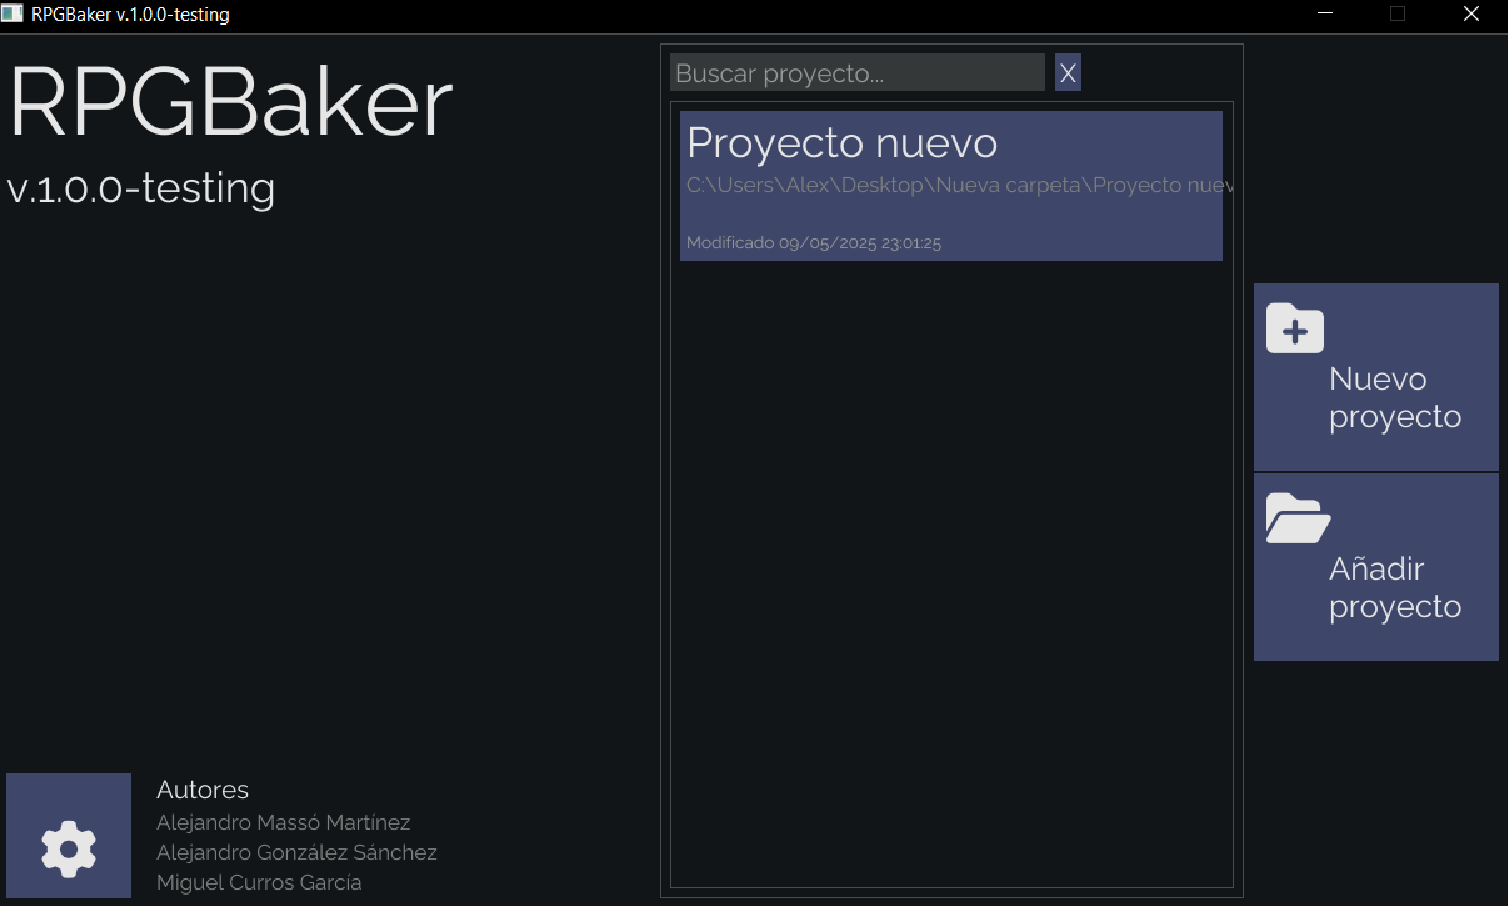
\includegraphics[width=0.45\textwidth]{Imagenes/Vectorial/welcomewindow}%
	\end{SubFloat}
	\qquad
	\begin{SubFloat}
		{\label{fig:eventwindow}%
		Ventana de edición de eventos de \baker.}%
		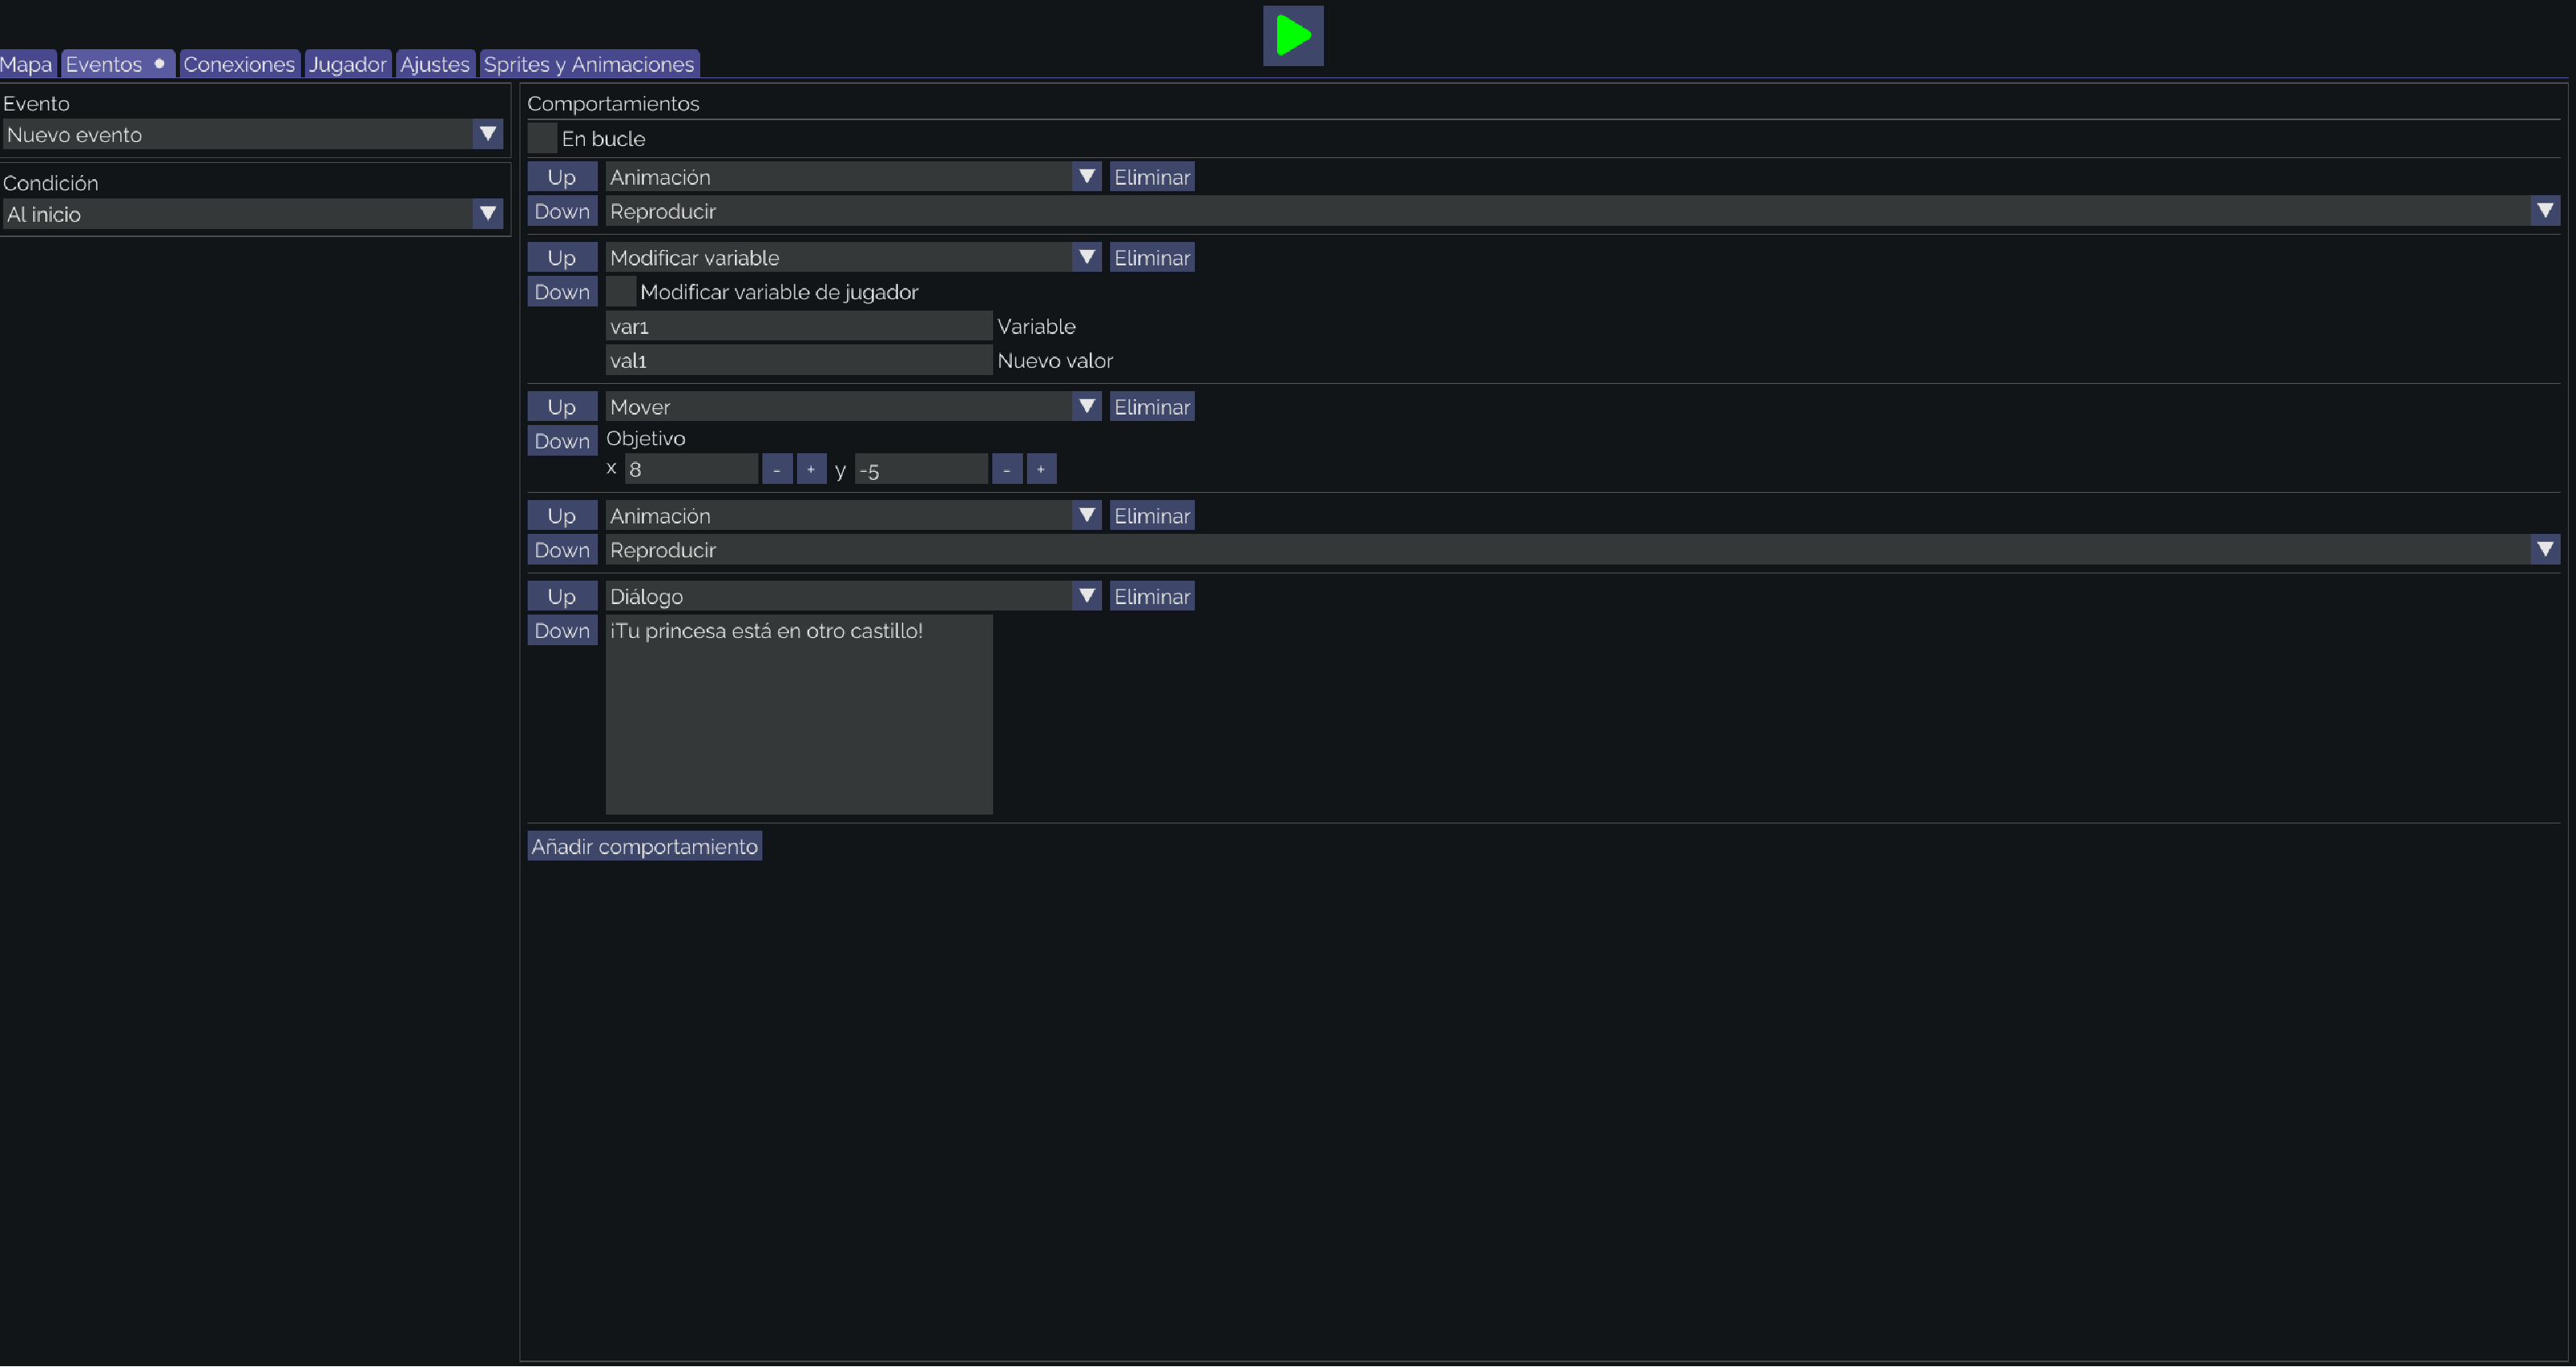
\includegraphics[width=0.45\textwidth]{Imagenes/Vectorial/eventos}%
	\end{SubFloat}
	%
	\begin{SubFloat}
		{\label{fig:conexiones}%
		Ventana de conexiones entre mapas de \baker.}%
		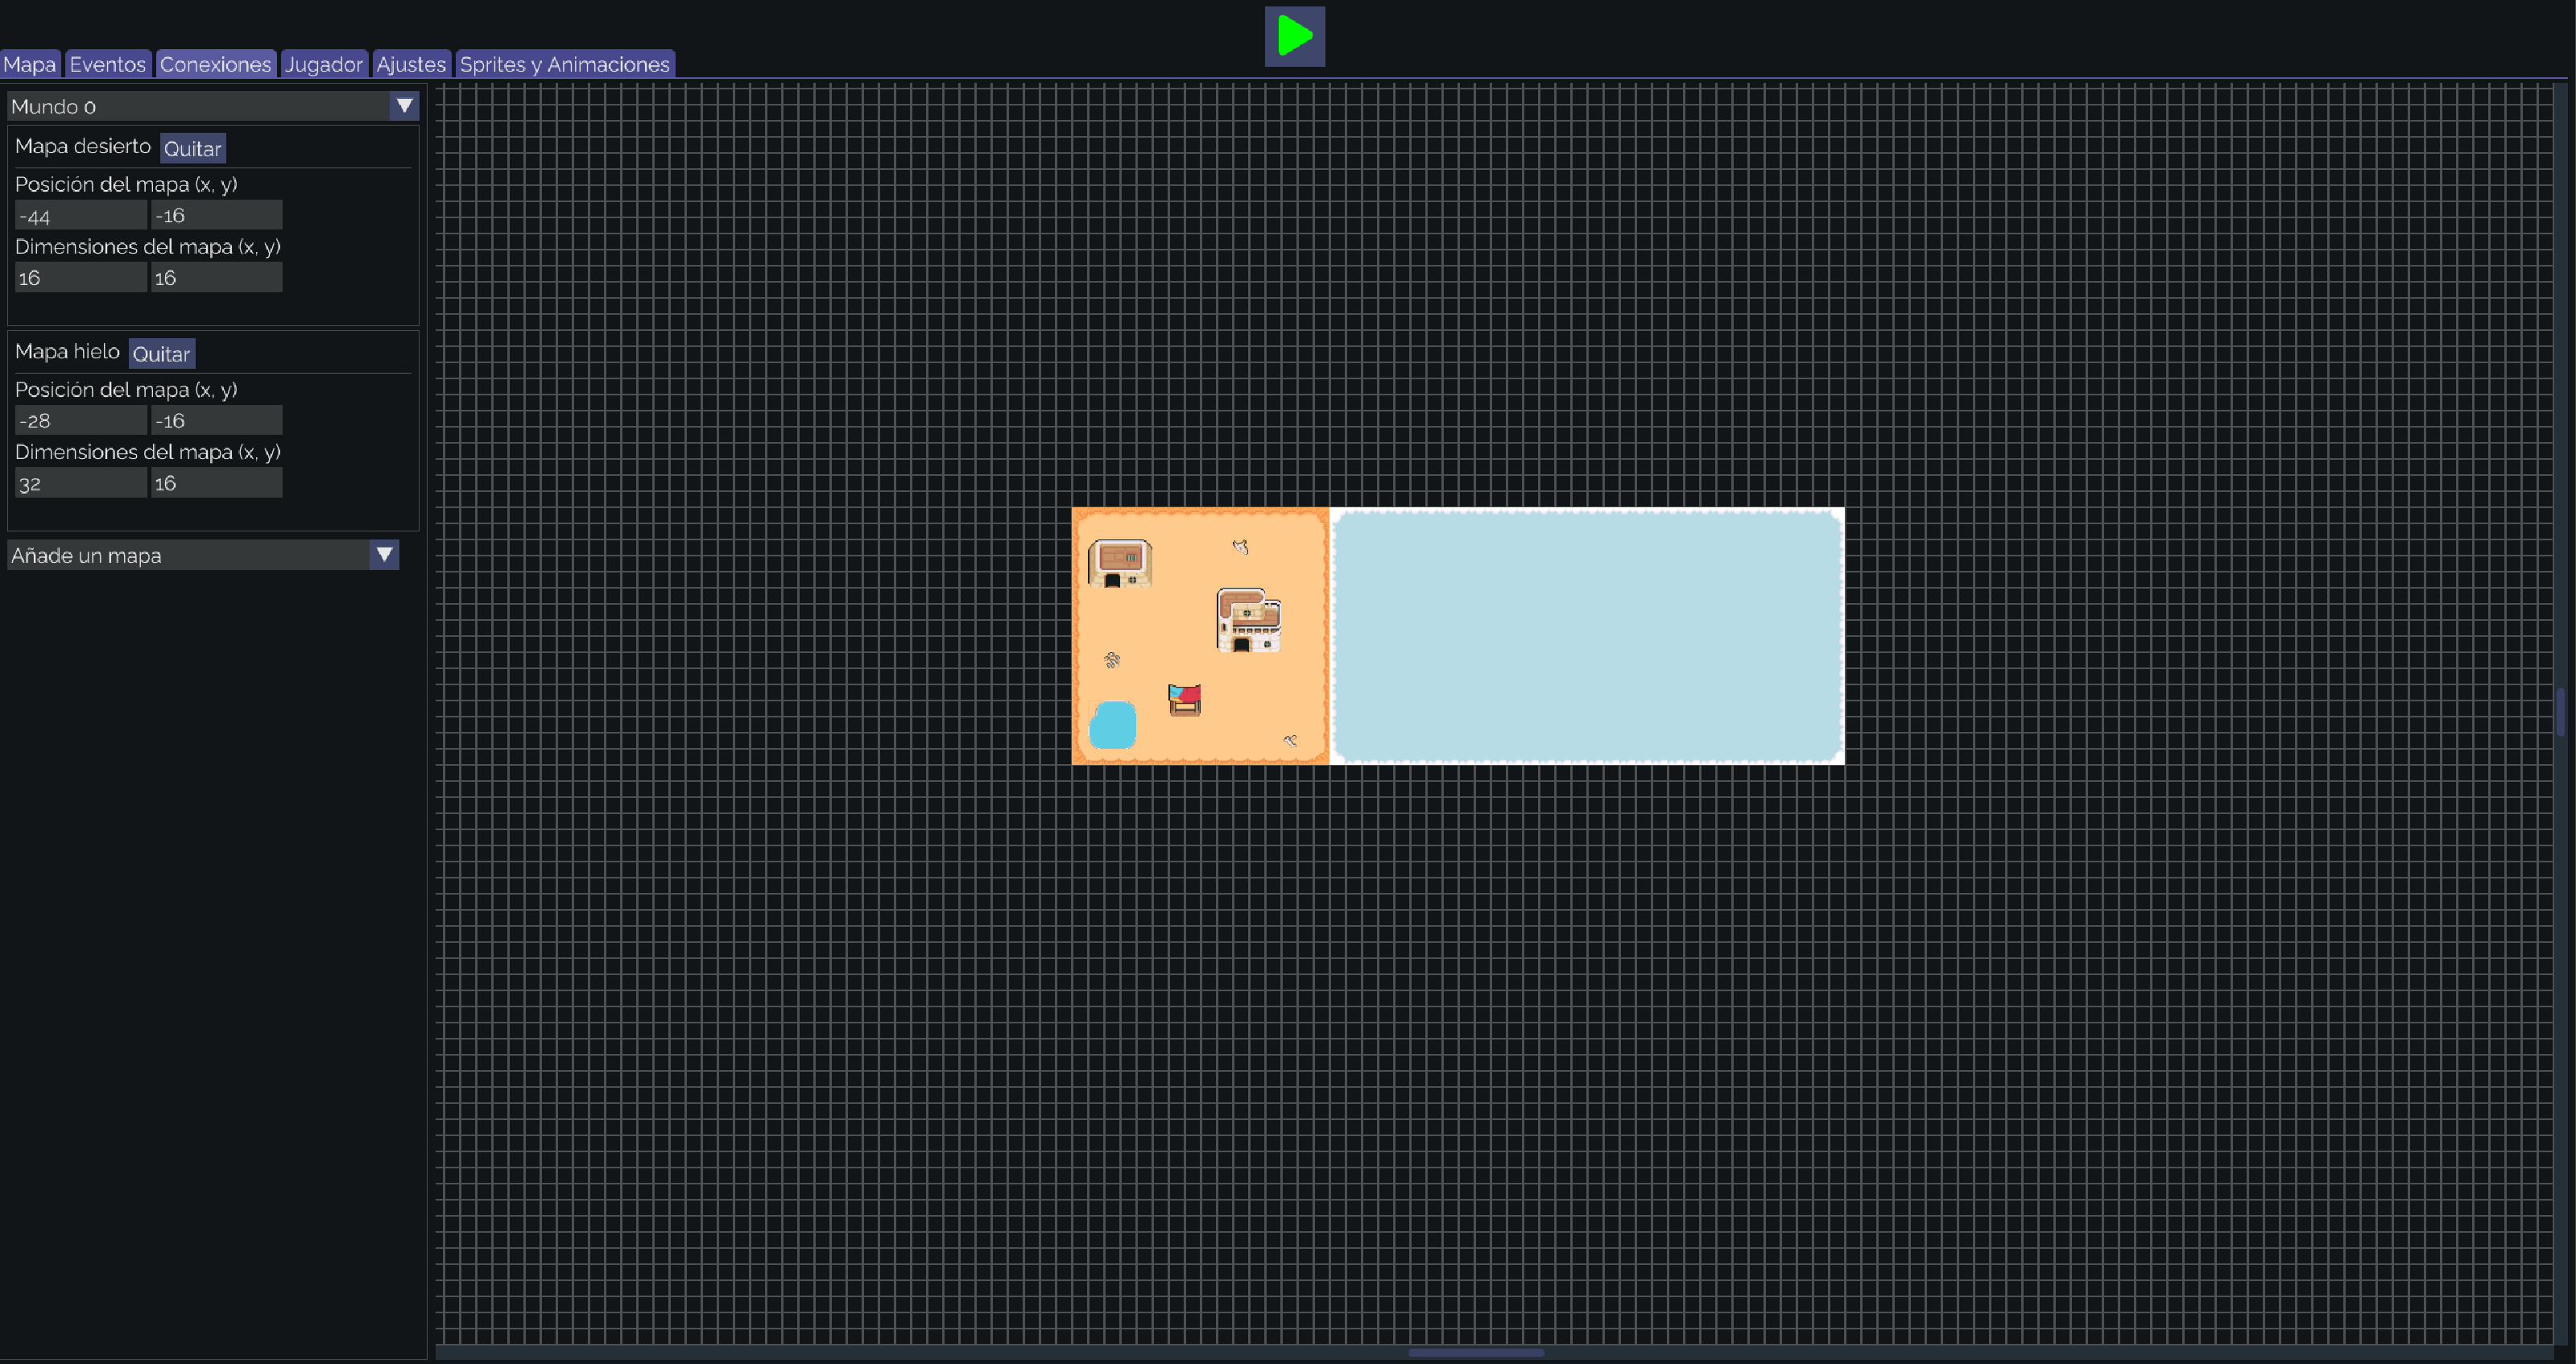
\includegraphics[width=0.45\textwidth]{Imagenes/Vectorial/conexiones}%
	\end{SubFloat}
	\qquad
	\begin{SubFloat}
		{\label{fig:playerwindow}%
		Ventana de edición del jugador de \baker.}%
		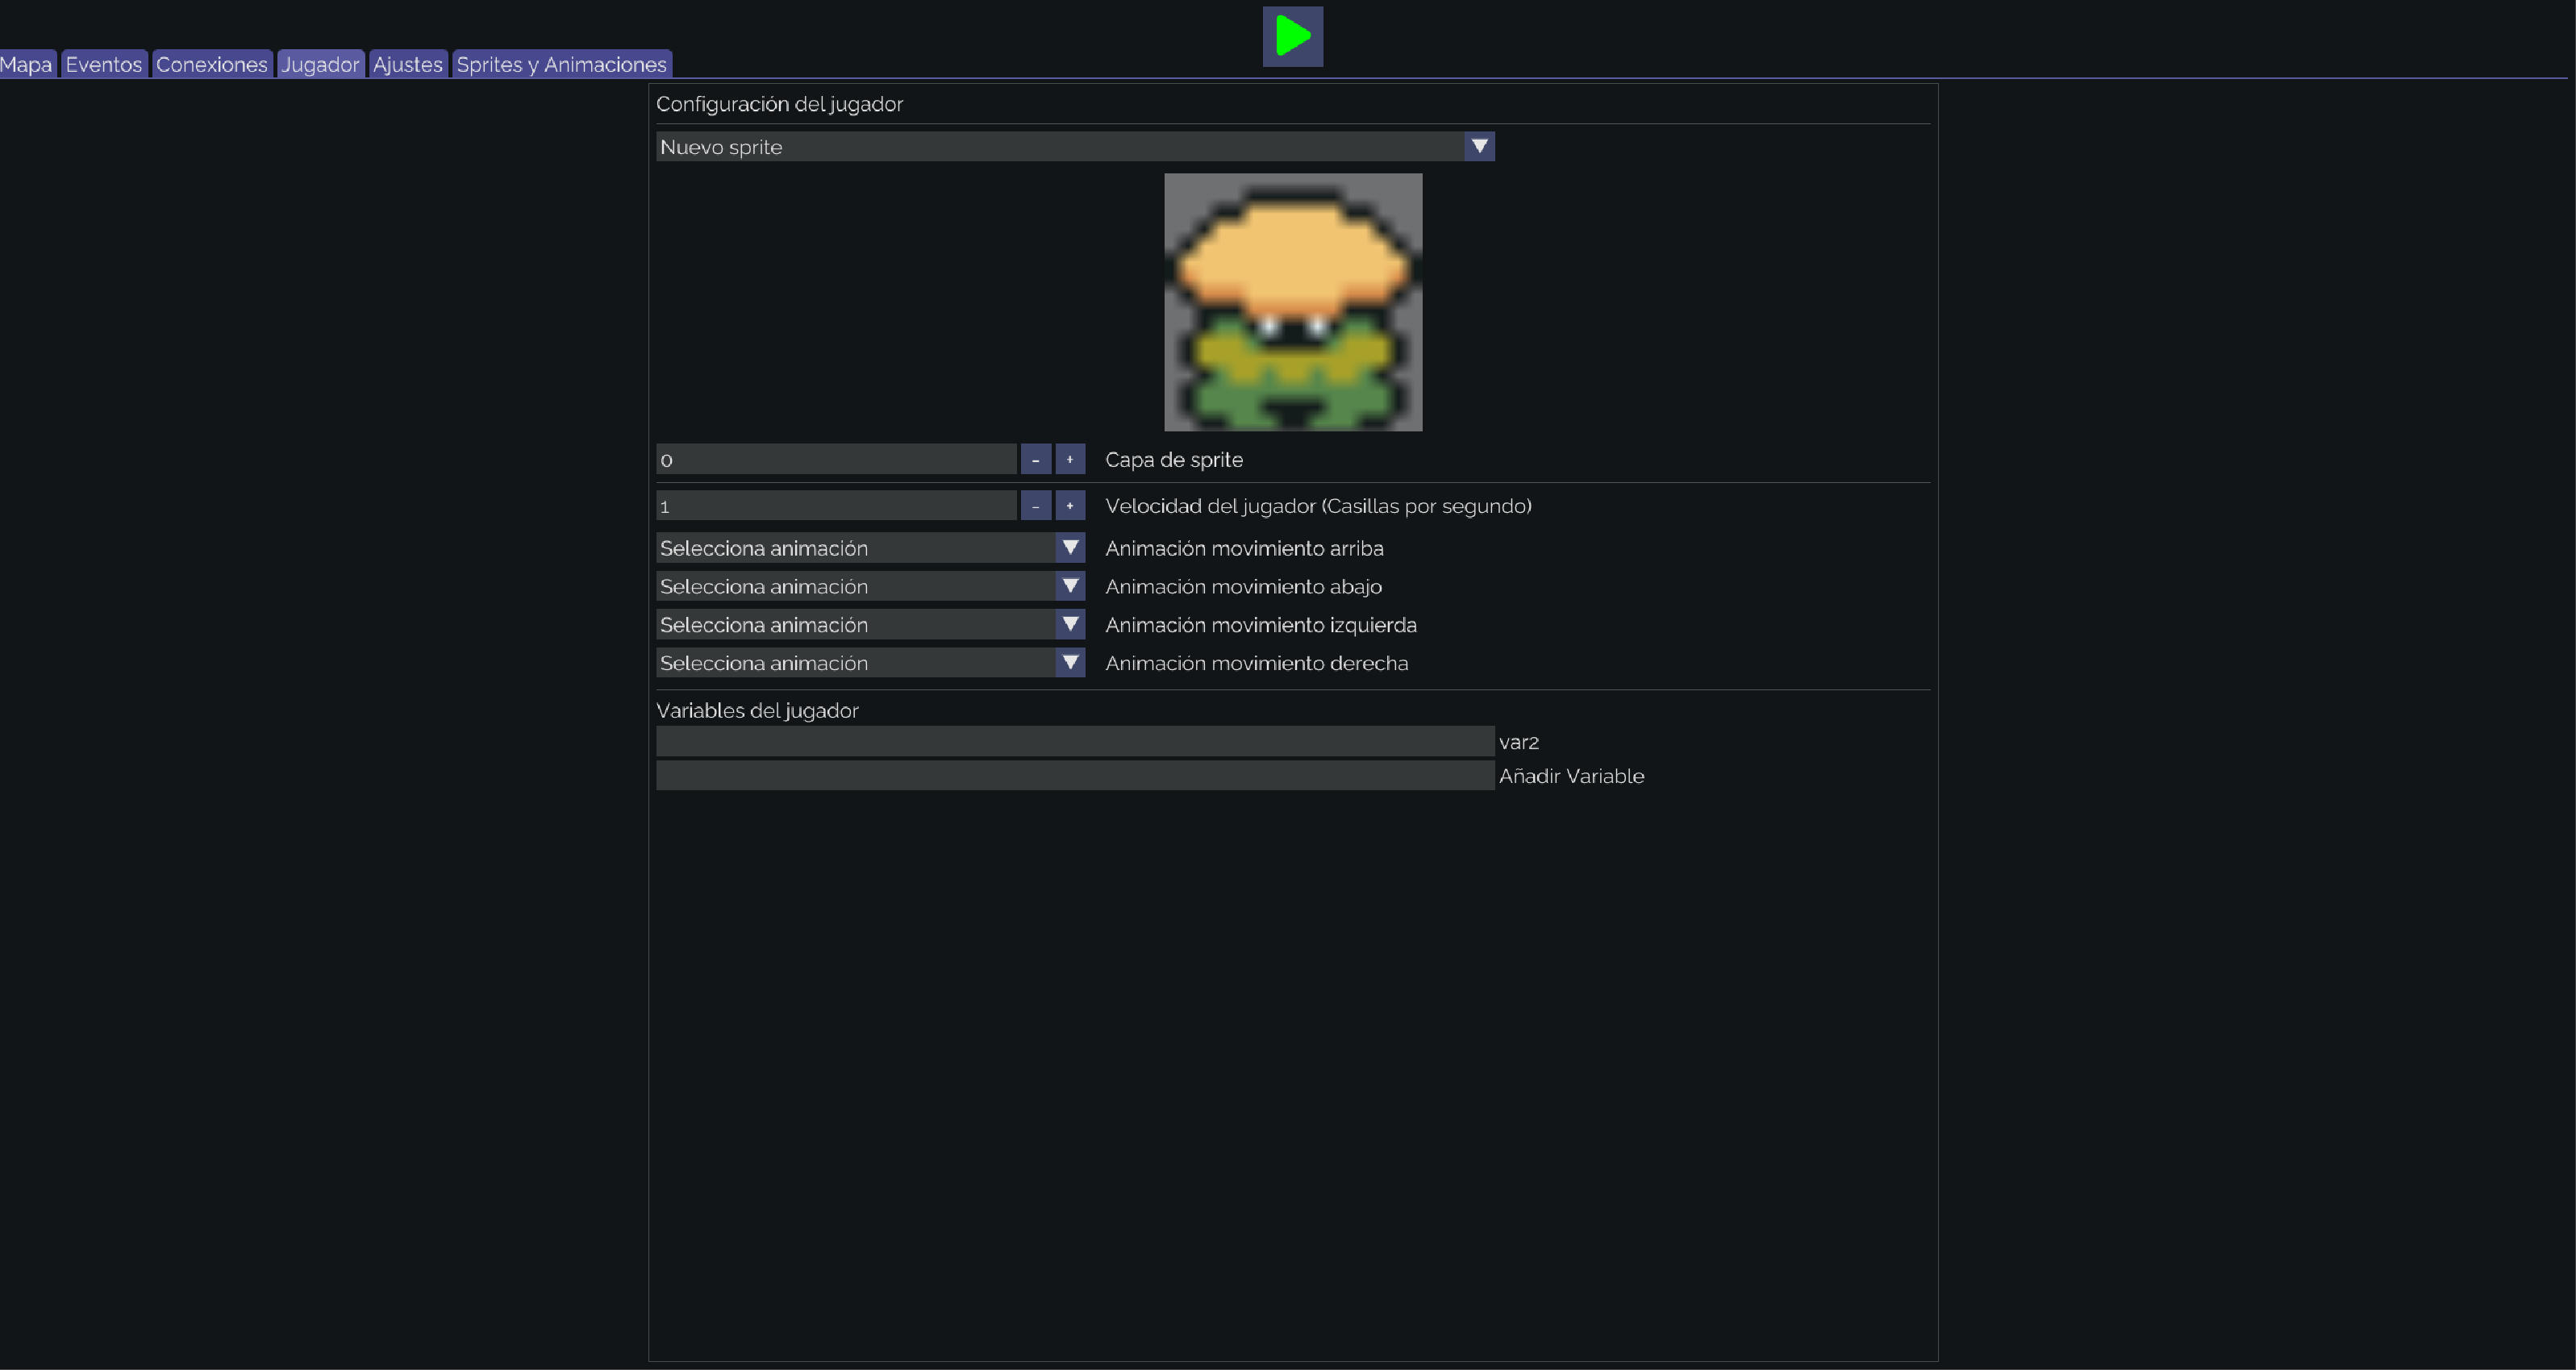
\includegraphics[width=0.45\textwidth]{Imagenes/Vectorial/jugador}%
	\end{SubFloat}
	\caption{Distintas ventanas del editor de \baker. \label{fig:menusbaker}}
\end{figure}

\begin{itemize}
	\item La ventana de bienvenida (figura \ref{fig:welcomewindow}), que permite la gestión de todos los proyectos creados por el usuario, así como crear uno nuevo y añadir otro ya existente, y también cambiar el idioma de la interfaz.
	\item La ventana principal de la aplicación, que permite la edición de un proyecto en concreto y está dividida en varias pestañas, cada una con una función distinta:
	\begin{itemize}
		\item El editor de mapas (figura \ref{fig:mapeditor}), permite la creación y modificación de un mapa utilizando diversos \textit{tilesets}. En la parte izquierda se encuentra el visor de \textit{tilesets}, que permite crear nuevas a partir de un fichero de imagen, editar las ya presentes o eliminarlas. En la parte central se encuentra el editor \textit{per se}, mostrándose una cuadrícula con el tamaño elegido por el usuario. Esta cuadrícula se puede ampliar y alejar, y tiene varios modos de visualización:
		\begin{itemize}
			\item Visualización de la capa actual exclusivamente.
			\item Visualización de la capa actual y las de abajo con transparencia.
			\item Visualización de la capa actual y las de abajo completamente opacas.
			\item Visualización de todas las capas en conjunto, empezando desde abajo hasta arriba.
		\end{itemize}
		Finalmente, en la parte derecha, se encuentra el editor de objetos, que permite crear y eliminar un objeto y agregarle o eliminarle un \textit{sprite}, un evento o una variable.
		\item El editor de eventos (figura \ref{fig:eventwindow}), que permite la creación y edición de eventos, añadiendo los comportamientos esperados y las condiciones de lanzamiento. Eventos complejos se encapsulan dentro de otros y todos se pueden ordenar por orden de prioridad de ejecución utilizando las flechas que aparecen al costado izquierdo.
		\item El editor de conexiones (figura \ref{fig:conexiones}), que permite crear mundos\footnote{Un mundo, en la jerarquía de nuestro Proyecto, es aquel elemento que puede contener diversos mapas.} y añadirle los mapas, modificando en la cuadrícula la posición final de cada uno de los mapas.
		\item El editor del jugador (figura \ref{fig:playerwindow}), que permite establecer ajustes del jugador, como por ejemplo su \textit{sprite}, sus animaciones de movimiento en las cuatro direcciones cardinales básicas y variables propias de este.
		\item El editor de ajustes, que permite editar información relevante al ejecutable final, como por ejemplo, el nombre de la ventana, las dimensiones que la cámara puede mostrar en pantalla de una sola vez, el mapa en el que empezará el jugador o la fuente por defecto que mostrarán los textos.
		\item El editor de \textit{sprites} y animaciones, que permite generar un \textit{sprite} a partir de un \textit{spritesheet} o de una imagen, estableciendo el \textit{offset} que se desee, y, posteriormente, a partir de los \textit{sprites}, poder generar una animación. El asistente de creación de animaciones contiene un visor en tiempo real de la animación, así como controles para poder navegar por los diversos fotogramas.
	\end{itemize}
\end{itemize}
%\chapter{Desarrollo del Proyecto}
\label{cap:desarrollo}

%\chapter{Descripción del Trabajo}
\label{cap:descripcionTrabajo}

Aquí comienza la descripción del trabajo realizado. Se deben incluir tantos capítulos como sea necesario para describir de la manera más completa posible el trabajo que se ha llevado a cabo. Como muestra la figura \ref{fig:sampleImage}, está todo por hacer.

\begin{figure}[h]
	\centering
	
\includegraphics[width = 0.5\textwidth]{Imagenes/Vectorial/Todo.pdf}
	\caption{Ejemplo de imagen}
	\label{fig:sampleImage}
\end{figure}

Si te sirve de utilidad,  puedes incluir tablas para mostrar resultados, tal como se ve en la tabla \ref{tab:sampleTable}.


\begin{table}
	\centering
	\begin{tabular}{c|c|c}
		\textbf{Col 1} & \textbf{Col 2} & \textbf{Col 3} \\
		\hline\hline
		3 & 3.01 & 3.50\\
		6 & 2.12 & 4.40\\
		1 & 3.79 & 5.00\\
		2 & 4.88 & 5.30\\
		4 & 3.50 & 2.90\\
		5 & 7.40 & 4.70\\
		\hline
	\end{tabular}
	\caption{Tabla de ejemplo}
	\label{tab:sampleTable}
\end{table}

%\include{Capitulos/Capitulo4}
%\include{Capitulos/Capitulo5}
\chapter{Evaluación y Conclusiones}
\label{cap:conclusiones}

Al conocer en profundidad cómo funcionan todos los sistemas del motor y el editor, no podemos tener la certeza de que estos funcionen como un usuario promedio esperaría. Por esto, realizar pruebas con usuarios sin sesgos es crucial para obtener la información de las posibles brechas entre los programas y esos usuarios. De cara a ofrecer una experiencia de uso agradable se analizarán las pruebas en busca de formas de mejorarla. Se buscarán distintos tipos de perfiles para obtener una mayor cantidad de datos sobre los posibles conflictos que estos tengan con los sistemas.

\section{Objetivo de la evaluación}
Los objetivos de las pruebas con usuarios son principalmente dos. El primero es evaluar si los usuarios entienden los sistemas y son capaces de usarlos cómodamente, es importante que el entorno sea agradable de usar para permitir que los usuarios entiendan las capacidades del mismo y las puedan aprovechar. El segundo es evaluar si cada usuario es capaz de usar el editor creativamente, de forma que los videojuegos que cree un usuario suponga una experiencia diferente a los que haga otro, comprobando así la flexibilidad de uso del editor.

\section{Metodología}
Para realizar estas pruebas, una vez se plantearon los objetivos, se diseñó cómo se iban a realizar. Cada usuario realizará las pruebas de manera individual en compañía de un supervisor, tendrán una duración estimada de una hora. A cada probador se le preguntan lo primero de todo su experiencia tanto jugando como creando videojuegos, haciendo énfasis en los RPG. Una vez con estos datos se le entregan varios ficheros al empezar la prueba, el ejecutable del editor, un paquete de recursos para no desaprovechar tiempo de la prueba buscando y una breve guía de uso del editor. En esta guía se explica brevemente el modo de uso de cada uno de los sistemas disponibles en el editor. Una vez con esto, el probador seguirá la guía para entender los mecanismos y podrá para utilizarlos a su libre albedrío.

\medskip

El investigador se encargará de registrar todas las interacciones destacables de los probadores con el editor, además de prestar ayuda si surge algún error con el programa a lo largo de las pruebas. Para poder observar una experiencia real, el investigador no podrá intervenir en las acciones del usuario más que en esos casos excepcionales con los errores o en momentos de bloqueo en los que el probador no es capaz de continuar por alguna brecha. Estas pruebas están pensadas para realizarse tanto en persona como telemáticamente a mayor comodidad de cada caso concreto. Una vez finalice la prueba se le pedirá al usuario una valoración general sobre los sistemas y su experiencia de uso aportando sus quejas e ideas.

\section{Resultados}

Los usuarios pueden agruparse en 3 categorías según su experiencia con los videojuegos y, en particular, con los RPG.

\smallskip 

En primer lugar, se encuentran los usuarios más ajenos al mundo de los videojuegos, con poca experiencia jugando a juegos en general y a juegos RPG en concreto. Con este tipo de usuario el objetivo es ver como de intuitivas son las herramientas y la UI de la aplicación del editor, así como ver si se entienden bien las instrucciones de las pruebas. Este primer grupo consiguió crear mapas con cierto sentido, pero la mayoría utilizó únicamente una o dos capas por lo que con esto quedaban un poco limitados a la hora del diseño. No invirtieron gran cantidad de tiempo explorando los tilesets e hicieron unos diseños más bien sencillos. Las configuraciones las entendieron bastante bien, y siguiendo la guía las consiguieron rellenar. A la hora de crear eventos se quedaron en los behaviours más sencillos y no intentaron crear eventos complejos usando variables y condiciones. En general la prueba fue satisfactoria y los resultados estaban dentro de lo esperado. 

\medskip

En segundo lugar, se tienen a usuarios que sí juegan a videojuegos y algunos incluso están relacionados con la industria, pero no tienen conocimientos de programación o de desarrollo más allá de sus áreas específicas. Estos si aprovecharon mucho más el apartado del mapeado, utilizando más capas y varios tilesets creando mapas mucho más interesantes. A la hora de los eventos se les insistió más que al primer grupo para que intentaran crear algunos eventos algo más complejos, pero al parecer no les quedaba tan claro como estructurarlos para aprovechar al máximo las funcionalidades y la mayoría se quedó en cosas algo más sencillas o tuvieron que recibir bastante ayuda por parte de los supervisores. Aunque los eventos no requieren conocimientos de programación, su estructura es similar a la de un sistema basado en lógica condicional, lo que exige más tiempo del que se disponía durante la prueba para entender cómo organizarlos correctamente. 

\medskip

Por último, está el grupo de gente que tiene conocimiento en el desarrollo de los videojuegos, incluso en el desarrollo de \textit{RPGMaker} específicamente, lo que fue muy interesante a la hora de obtener \textit{feedback} comparativo. Este grupo entendió bien las herramientas de mapeado y señaló que echaba en falta algunas más avanzadas que agilizaran un poco el proceso, como la opción de seleccionar varios \textit{tiles} a la vez o de rellenar zonas con \textit{tiles} de un tipo. También señalaron lo lento que es el proceso de creación de \textit{sprites} y animaciones, proponiendo algún tipo de automatización de este como ocurre con los \textit{tilesets}. En cuanto a los eventos lograron entender como montar estructuras más avanzadas, lo cual fue un resultado positivo. 

\medskip

Adicionalmente a todas las observaciones y el \textit{feedback} recibido, las pruebas también fueron útiles para detectar varios \textit{bugs} y cosas que no estaban funcionando correctamente, lo que fue de gran ayuda de cara a dar un pulido final a la versión del editor. 

\section{Análisis de los resultados y conclusiones}
Aunque las pruebas no alcanzaron la extensión ni la variedad deseables debido a limitaciones logísticas, se pueden sacar algunas conclusiones interesantes de cara al desarrollo actual y sobre todo a un posible trabajo futuro.

\smallskip 

Una de las prioridades identificadas es la mejora de la experiencia de diseño de mapas y de creación de \textit{sprites} y animaciones. Con este objetivo, se proponen las siguientes mejoras funcionales:

\begin{itemize}
	\item Incorporar la posibilidad de seleccionar varios \textit{tiles} simultáneamente y pintarlos en el mapa de forma conjunta. 

	\item Añadir una herramienta para rellenar automáticamente una zona completa con el \textit{tile} seleccionado. 

	\item Permitir la selección de \textit{tiles} directamente desde el mapa, sin necesidad de localizarlos manualmente en el \textit{tileset}. 

	\item Incluir una función para deshacer la última edición realizada. 

	\item Automatizar el proceso de creación de múltiples \textit{sprites} y su conversión en animaciones a partir de una única fuente, de manera similar al funcionamiento del editor de \textit{tilesets}. 
\end{itemize}

Además, se considera conveniente implementar mejoras en forma de \textit{tooltips} en la sección de eventos, con el objetivo de explicar de manera clara todas las funcionalidades disponibles. También se sugiere incluir eventos predefinidos que sirvan como ejemplos prácticos para facilitar su comprensión y uso.



\begin{otherlanguage}{english}
\chapter*{Evaluation and analysis}
\label{cap:conclusions}
\addcontentsline{toc}{chapter}{Evaluation and analysis}

By thoroughly understanding how all the systems of the engine and the editor work, it cannot be guaranteed that they will function as an average user expects. For this reason, conducting unbiased user testing is crucial to gather information about the possible gaps between the programs and those users. With the goal of providing a pleasant user experience, the tests will be analyzed to find ways to improve it. Different types of user profiles will be sought to obtain a greater amount of data about the potential conflicts they may have with the systems.

\section*{Evaluation objective}
The objectives of the user tests are primarily two. The first is to evaluate whether users understand the systems and are able to use them comfortably. It is important that the environment is pleasant to use in order to allow users to understand its capabilities and take full advantage of them. The second is to assess whether each user is capable of using the editor creatively, in such a way that the video games created by one user offer a different experience than those made by another, thus verifying the editor’s flexibility.

\section*{Methodology}
To conduct these tests, once the objectives were established, the testing procedure was designed. Each user will perform the tests individually, accompanied by a supervisor, with an estimated duration of one hour.

\smallskip

At the start, each tester is first asked about their experience both playing and creating video games, with a focus on RPGs. After gathering this information, they are given several files: the editor executable, a resource package to avoid wasting time searching during the test, and a brief user guide for the editor.

\smallskip

This guide provides a concise explanation of how to use each of the systems available in the editor. With this information, the tester follows the guide to understand the mechanics and then is free to use them as they wish.

\medskip

The researcher will be responsible for recording all notable interactions between the testers and the editor, as well as providing assistance if any errors occur during the tests. To capture a realistic user experience, the researcher will not intervene in the user’s actions except in exceptional cases—such as program errors or situations where the tester is stuck and unable to continue due to a problem.

\smallskip

These tests are designed to be conducted either in person or remotely, depending on what is most convenient for each individual case. Once the test is complete, the user will be asked to provide general feedback on the systems and their experience, including any complaints or suggestions.

\section*{Results}

Users can be grouped into three categories based on their experience with video games, and in particular, with RPGs.

\smallskip

First, there are users who are least familiar with the world of video games, with little experience playing games in general and, in particular, RPGs. With this type of user, the goal is to evaluate how intuitive the tools and the editor’s user interface are, as well as to verify if the test instructions are well understood. This first group managed to create maps that made some sense, but most used only one or two layers, which somewhat limited their design. They did not spend much time exploring the tilesets and made rather simple designs. They understood the configurations quite well and, following the guide, were able to complete them. When creating events, they stuck to the simplest behaviors and did not attempt to create complex events using variables and conditions. Overall, the test was satisfactory and the results were within expectations.

\medskip

Second, there are users who do play video games and some are even related to the industry, but they lack programming or development knowledge beyond their specific areas. These users made much greater use of the mapping section, using more layers and multiple tilesets to create much more interesting maps. Regarding events, they were encouraged more than the first group to try creating somewhat more complex events, but it seems they were not quite clear on how to structure them to fully leverage the functionalities, and most remained with simpler events or required significant help from supervisors. Although events do not require programming knowledge, their structure is similar to a system based on conditional logic, which demands more time than was available during the test to understand how to organize them properly.

\medskip

Finally, there is the group of people with knowledge in video game development, including specific experience with RPGMaker development, which was very useful for obtaining comparative feedback. This group understood the mapping tools well and pointed out the lack of some more advanced options that could speed up the process, such as the ability to select multiple tiles at once or fill areas with tiles of the same type. They also mentioned that the process of creating sprites and animations is slow, proposing some kind of automation similar to that available for tilesets. Regarding events, they managed to understand how to build more advanced structures, which was a positive outcome.

\medskip

In addition to all the observations and feedback received, the tests also helped detect several bugs and issues that were not working properly, which was very helpful for polishing the final version of the editor.

\section*{Results analysis and conclusions}
Although the tests did not reach the desired length or variety due to logistical limitations, some interesting conclusions can be drawn for the current development and, especially, for potential future work.

\smallskip

One of the identified priorities is improving the experience of map design and the creation of sprites and animations. To this end, the following functional improvements are proposed:

\begin{itemize}
	\item Incorporate the ability to select multiple tiles simultaneously and paint them together on the map.
	\item Add a tool to automatically fill an entire area with the selected tile.
	\item Allow tile selection directly from the map, without needing to manually locate them in the tileset.
	\item Include an undo function to revert the last edit made.
	\item Automate the process of creating multiple sprites and converting them into animations from a single source, similar to how the tileset editor works.
\end{itemize}

Additionally, it is considered advisable to implement improvements in the form of tooltips in the events section, aimed at clearly explaining all available functionalities. It is also suggested to include predefined events that serve as practical examples to facilitate understanding and use.

\end{otherlanguage}
\chapter{Evaluación y Conclusiones}
\label{cap:conclusiones}

Al conocer en profundidad cómo funcionan todos los sistemas del motor y el editor, no podemos tener la certeza de que estos funcionen como un usuario promedio esperaría. Por esto, realizar pruebas con usuarios sin sesgos es crucial para obtener la información de las posibles brechas entre los programas y esos usuarios. De cara a ofrecer una experiencia de uso agradable se analizarán las pruebas en busca de formas de mejorarla. Se buscarán distintos tipos de perfiles para obtener una mayor cantidad de datos sobre los posibles conflictos que estos tengan con los sistemas.

\section{Objetivo de la evaluación}
Los objetivos de las pruebas con usuarios son principalmente dos. El primero es evaluar si los usuarios entienden los sistemas y son capaces de usarlos cómodamente, es importante que el entorno sea agradable de usar para permitir que los usuarios entiendan las capacidades del mismo y las puedan aprovechar. El segundo es evaluar si cada usuario es capaz de usar el editor creativamente, de forma que los videojuegos que cree un usuario suponga una experiencia diferente a los que haga otro, comprobando así la flexibilidad de uso del editor.

\section{Metodología}
Para realizar estas pruebas, una vez se plantearon los objetivos, se diseñó cómo se iban a realizar. Cada usuario realizará las pruebas de manera individual en compañía de un supervisor, tendrán una duración estimada de una hora. A cada probador se le preguntan lo primero de todo su experiencia tanto jugando como creando videojuegos, haciendo énfasis en los RPG. Una vez con estos datos se le entregan varios ficheros al empezar la prueba, el ejecutable del editor, un paquete de recursos para no desaprovechar tiempo de la prueba buscando y una breve guía de uso del editor. En esta guía se explica brevemente el modo de uso de cada uno de los sistemas disponibles en el editor. Una vez con esto, el probador seguirá la guía para entender los mecanismos y podrá para utilizarlos a su libre albedrío.

\medskip

El investigador se encargará de registrar todas las interacciones destacables de los probadores con el editor, además de prestar ayuda si surge algún error con el programa a lo largo de las pruebas. Para poder observar una experiencia real, el investigador no podrá intervenir en las acciones del usuario más que en esos casos excepcionales con los errores o en momentos de bloqueo en los que el probador no es capaz de continuar por alguna brecha. Estas pruebas están pensadas para realizarse tanto en persona como telemáticamente a mayor comodidad de cada caso concreto. Una vez finalice la prueba se le pedirá al usuario una valoración general sobre los sistemas y su experiencia de uso aportando sus quejas e ideas.

\section{Resultados}

Los usuarios pueden agruparse en 3 categorías según su experiencia con los videojuegos y, en particular, con los RPG.

\smallskip 

En primer lugar, se encuentran los usuarios más ajenos al mundo de los videojuegos, con poca experiencia jugando a juegos en general y a juegos RPG en concreto. Con este tipo de usuario el objetivo es ver como de intuitivas son las herramientas y la UI de la aplicación del editor, así como ver si se entienden bien las instrucciones de las pruebas. Este primer grupo consiguió crear mapas con cierto sentido, pero la mayoría utilizó únicamente una o dos capas por lo que con esto quedaban un poco limitados a la hora del diseño. No invirtieron gran cantidad de tiempo explorando los tilesets e hicieron unos diseños más bien sencillos. Las configuraciones las entendieron bastante bien, y siguiendo la guía las consiguieron rellenar. A la hora de crear eventos se quedaron en los behaviours más sencillos y no intentaron crear eventos complejos usando variables y condiciones. En general la prueba fue satisfactoria y los resultados estaban dentro de lo esperado. 

\medskip

En segundo lugar, se tienen a usuarios que sí juegan a videojuegos y algunos incluso están relacionados con la industria, pero no tienen conocimientos de programación o de desarrollo más allá de sus áreas específicas. Estos si aprovecharon mucho más el apartado del mapeado, utilizando más capas y varios tilesets creando mapas mucho más interesantes. A la hora de los eventos se les insistió más que al primer grupo para que intentaran crear algunos eventos algo más complejos, pero al parecer no les quedaba tan claro como estructurarlos para aprovechar al máximo las funcionalidades y la mayoría se quedó en cosas algo más sencillas o tuvieron que recibir bastante ayuda por parte de los supervisores. Aunque los eventos no requieren conocimientos de programación, su estructura es similar a la de un sistema basado en lógica condicional, lo que exige más tiempo del que se disponía durante la prueba para entender cómo organizarlos correctamente. 

\medskip

Por último, está el grupo de gente que tiene conocimiento en el desarrollo de los videojuegos, incluso en el desarrollo de \textit{RPGMaker} específicamente, lo que fue muy interesante a la hora de obtener \textit{feedback} comparativo. Este grupo entendió bien las herramientas de mapeado y señaló que echaba en falta algunas más avanzadas que agilizaran un poco el proceso, como la opción de seleccionar varios \textit{tiles} a la vez o de rellenar zonas con \textit{tiles} de un tipo. También señalaron lo lento que es el proceso de creación de \textit{sprites} y animaciones, proponiendo algún tipo de automatización de este como ocurre con los \textit{tilesets}. En cuanto a los eventos lograron entender como montar estructuras más avanzadas, lo cual fue un resultado positivo. 

\medskip

Adicionalmente a todas las observaciones y el \textit{feedback} recibido, las pruebas también fueron útiles para detectar varios \textit{bugs} y cosas que no estaban funcionando correctamente, lo que fue de gran ayuda de cara a dar un pulido final a la versión del editor. 

\section{Análisis de los resultados y conclusiones}
Aunque las pruebas no alcanzaron la extensión ni la variedad deseables debido a limitaciones logísticas, se pueden sacar algunas conclusiones interesantes de cara al desarrollo actual y sobre todo a un posible trabajo futuro.

\smallskip 

Una de las prioridades identificadas es la mejora de la experiencia de diseño de mapas y de creación de \textit{sprites} y animaciones. Con este objetivo, se proponen las siguientes mejoras funcionales:

\begin{itemize}
	\item Incorporar la posibilidad de seleccionar varios \textit{tiles} simultáneamente y pintarlos en el mapa de forma conjunta. 

	\item Añadir una herramienta para rellenar automáticamente una zona completa con el \textit{tile} seleccionado. 

	\item Permitir la selección de \textit{tiles} directamente desde el mapa, sin necesidad de localizarlos manualmente en el \textit{tileset}. 

	\item Incluir una función para deshacer la última edición realizada. 

	\item Automatizar el proceso de creación de múltiples \textit{sprites} y su conversión en animaciones a partir de una única fuente, de manera similar al funcionamiento del editor de \textit{tilesets}. 
\end{itemize}

Además, se considera conveniente implementar mejoras en forma de \textit{tooltips} en la sección de eventos, con el objetivo de explicar de manera clara todas las funcionalidades disponibles. También se sugiere incluir eventos predefinidos que sirvan como ejemplos prácticos para facilitar su comprensión y uso.



\begin{otherlanguage}{english}
\chapter*{Conclusions and Future Work}
\label{cap:conclusions}
\addcontentsline{toc}{chapter}{Conclusions and Future Work}

Conclusions and future lines of work. This chapter contains the translation of Chapter \ref{cap:conclusiones}.



\end{otherlanguage}

%%%%%%%%%%%%%%%%%%%%%%%%%%%%%%%%%%%%%%%%%%%%%%%%%%%%%%%%%%%%%%%%%%%%%%%%%%%
% Si el TFG se escribe en inglés, comentar las siguientes líneas 
% porque no es necesario incluir nuevamente las Conclusiones en inglés
%%%%%%%%%%%%%%%%%%%%%%%%%%%%%%%%%%%%%%%%%%%%%%%%%%%%%%%%%%%%%%%%%%%%%%%%%%%

\chapter{Contribuciones Personales}
\label{cap:contribucionesPersonales}
\addcontentsline{toc}{chapter}{Contribuciones Personales}

\section*{Miguel Curros García}
Mis tareas en el proyecto se centraron en el diseño y desarrollo del motor genérico de videojuegos así como dentro del apartado de \textit{gameplay} todo lo relacionado con el sistema de eventos, tanto a nivel de motor como de editor. Adicionalmente, también creé la gestión de persistencia con lectura y escritura de los archivos de datos específicos del editor y parte del proceso de \textit{build}.

\medskip

En primer lugar, participé en conjunto con Alejandro González en la fase de diseño del motor donde dejamos bien claras cuáles serían las distintas capas de abstracción de la implementación. Desde el principio teníamos claro que la base del motor iba a estar basada en una arquitectura EC (\textit{Entity-Component}), construyendo el resto de las funcionalidades alrededor. Comenzamos a definir cómo estructuraríamos esa arquitectura a través de un diagrama \textit{UML} donde definimos tanto los distintos módulos que formarían el motor como la forma en la que se conectarían las partes más básicas de este con las funcionalidades específicas de \textit{gameplay}.

\medskip
 
A continuación, comencé con el desarrollo de este centrándome en los apartados de carga y gestión de recursos, audio y colisiones. Comenzando con la gestión de recursos, esta es una parte crucial del motor al estar este dirigido por datos; todo aquello que se quiere que ocurra en un juego estará definido en los datos a interpretar al motor.
Esta parte tiene 3 partes clave: \texttt{Resource}, \texttt{ResourceHandler} y \texttt{ResourceMemoryManager}. Cada una de esas clases se encarga de una parte clave de la carga y descarga de recursos. 
\begin{itemize}
	\item \texttt{Resource} servirá de clase base para todos los tipos de recursos que se quieran cargar, cada uno de ellos implementará cómo se carga y descarga desde los archivos de datos.
	\item \texttt{ResourceHandler} será a quien recurran las distintas partes del motor que necesiten cualquier tipo de recurso. A través de la ruta a un recurso de un tipo especificado dará acceso a una instancia conteniendo ese mismo recurso cargado.
	\item Por último, \texttt{ResourceMemoryManager} se encargará de gestionar cuánta memoria está siendo ocupada en este momento por los recursos. A partir de un límite especificado en un archivo de configuración esta clase se encargará de que no se supere ese umbral de memoria máxima ocupada por los recursos. Si se solicitara un recurso y no hubiera memoria suficiente para cargarlo a través de un algoritmo LRU se irá liberando memoria de otros recursos hasta que haya suficiente para cargar el nuevo. Con esto, conseguí estructurar la carga de recursos bajo demanda que evitaría posibles largos tiempos de espera los juegos.
\end{itemize}

\medskip

Una vez esto estaba listo desarrollé el sistema de sonido que permitiría el control sobre la reproducción de archivos de audio dentro de los juegos. Para esto decidimos usar el nuevo sistema de audio de \textit{SDL3} que cumplía todas nuestras necesidades. Nuestro objetivo con este sistema era la implementación de un componente \texttt{AudioSource} a través del que gestionar la reproducción de un archivo de audio. Además, queríamos que cada uno de estos \texttt{AudioSource} pudieran estar asociados a un conjunto de sonidos, pudiendo tener de esta forma un control más profundo del volumen; pues es típico y útil en los videojuegos permitir al jugador controlar el volumen general, de la música o de los efectos por separado.

\smallskip

Para poder reproducir un sonido creé una clase \texttt{AudioClip} que se encargaría de envolver las funcionalidades de \texttt{SDL\_AudioStream}; la base de la reproducción de sonidos en \textit{SDL3}; y ofrecer una interfaz acorde a nuestras necesidades. Para poder asignar estas pistas a distintos conjuntos de sonidos implementé la clase \texttt{AudioMixer}, que tendría un control de volumen asociado que se aplicaría a cada uno de sus \texttt{AudioClip}. Una vez con estas clases básicas pude implementar \texttt{AudioSource} que las utilizaría para ofrecer su funcionalidad esperada.

\medskip

Por último en la base del motor, para la detección y gestión de colisiones buscábamos algo sencillo. Por el tipo de videojuegos que ofrecemos implementar basta con comprobaciones de colisiones entre formas rectangulares. Son comprobaciones sencillas y \textit{SDL} ya ofrece funciones para comprobar si dos rectángulos tienen intersección. Con esto, la implementación de un componente \texttt{Collider} fue sencilla. A través de una clase \texttt{CollisionManager}, en cada actualización del juego se comprobarían las colisiones entre estos \texttt{Collider}. En estas comprobaciones se guardaría la información de qué \texttt{Collider} está colisionando, acaba de empezar a colisionar o acaba de dejar de colisionar con otro. De esta manera se ofrece un control sencillo para implementar comprobaciones dependientes de colisiones entre elementos de juego.

\medskip

Una vez terminamos el apartado del motor genérico comenzamos con el desarrollo de partes específicas de \textit{GamePlay} donde centré mis aportaciones en el sistema de eventos. De cara a ofrecer una experiencia personalizable de crear un videojuego sin necesidad de programar un punto clave era nuestro sistema de eventos. Este se centra alrededor del componente \texttt{EventHandler} que sirve como conjunto de eventos de una entidad. Cada \texttt{Event} está compuesto por una condición, \texttt{EventCondition}, y comportamientos, \texttt{EventBehaviour}.
\begin{itemize}
	\item Comenzando por las condiciones, estas se encargan de manifestar si el estado del juego es el que esperan. Para ello, cada una de las condiciones debe implementar sus propias comprobaciones, esto lo hice a través de un sistema de herencia. Además, igual que pasa con los componentes, cada una de estas condiciones deben poder crearse a partir de los datos proporcionados por el juego, por esta razón creé una clase \texttt{EventConditionFactory}, que se encargaría de instanciar el tipo correspondiente de \texttt{EventCondition} dado un identificador.
	\item Los comportamientos decidimos que estuvieran implementados en \textit{Lua}. De esta manera se podrían ampliar las funcionalidades de un juego sin necesidad de recompilar el motor, ofreciendo una experiencia más flexible. Para implementarlo de la manera que diseñamos era necesario poder tener algún tipo de POO (Programación orientada a objetos) en \textit{Lua}, pero no es algo que ofrezca el lenguaje por defecto. A través de asignar funciones a tablas y modificando sus \textit{metatablas} pude obtener un comportamiento similar a las clases y la herencia. A partir de esa base implementé la clase \texttt{EventBehaviour} en \textit{C++} envolviendo a cada instancia que hubiera en una escena de los distintos comportamientos implementados en \textit{Lua}. Además de esto, para poder implementar cada uno de los comportamientos fue necesario definir desde \textit{C++} qué clases y cómo se podían modificar dentro de las implementaciones de estos en \textit{Lua}.
\end{itemize}

\medskip

Cuando esto estuvo listo comencé con el desarrollo del editor donde creé la gestión de persistencia con lectura y escritura de los archivos de datos específicos del editor. Estos datos decidimos que íbamos a guardarlos también en \textit{Lua} pues nos sería más sencillo de implementar al tener ya la infraestructura montada para ello. Gracias a la clase del editor \texttt{LuaManager} creada por Alejandro Massó, que permite acceder a tablas de \textit{Lua} de un archivo, crear nuevas y guardar estas en nuevos archivos, la tarea consistió en escribir y leer estas tablas. Cada vez que se quisiera salvar un proyecto cada uno de sus recursos guardarían sus parámetros en nuevas tablas de \textit{Lua} que se escribirían en archivos en subdirectorios específicos dentro de un directorio \comillas{projectfiles} dentro de la ruta del proyecto.

\medskip
 
A continuación desarrollé todo el apartado de Eventos, desde la creación, edición y posterior traducción a archivos preparados para ser leídos por el motor. Para este apartado lo primero que hice fue crear una nueva pestaña en el editor, la pestaña de edición de eventos. En esta se podría ver un desplegable donde escoger un evento, una sección donde se mostraría la condición del evento y otra sección donde se mostrarían los comportamientos. 
La parte de creación y selección de eventos fue sencilla, aprovechando que Alejandro Massó ya había implementado la creación y selección de mapas, reutilicé el código que pude para esta parte. Para hacer los apartados de la condición y los comportamientos, igual que con la condición en el motor, tuve que crear factorías que permitieran crear los distintos tipos de instancias de cada uno de estos a partir de identificadores. Esto es porque cada condición y cada comportamiento debe definir en el editor su propia clase, ya que su persistencia e interfaz gráfica difieren entre sí, de modo que requieren implementaciones distintas; además por esa misma persistencia es por lo que se necesita la factoría, cada evento puede tener cualquier tipo de condición o comportamiento y se debe poder reconstruir al abrir un proyecto guardado.

\medskip

Una vez completé todas las interfaces gráficas y la persistencia de todos los tipos de condiciones y comportamientos comencé con el proceso de \textit{build}; convertir estos datos a la sintaxis que el motor reconoce. En el caso de las condiciones fue sencillo, pues el formato en el que guardan su información en el editor es casi idéntico a lo que necesita el motor. Lo que refiere a los comportamientos no es así, hubo dos puntos clave en este apartado: dependencias de componentes y formato de escritura. Algunos de los comportamientos en el motor funcionan por su cuenta, es decir, con que existan dentro de su \texttt{EventHandler} cumplirán su función sin problema; en cambio hay otros que necesitan otros componentes para funcionar también de modo que, para que su proceso de \textit{build} fuera correcto necesitaban indicarle a su entidad que escribiera los componentes faltantes con los parámetros correctos. Por último, a diferencia del resto de proceso de \textit{build} este apartado no podía hacer uso del mecanismo que usamos para escribir el resto de tablas de \textit{Lua}. Esto ocurre porque no estamos añadiendo otra tabla al uso, se necesita la llamada a la construcción de ese \texttt{EventBehaviour} porque el mecanismo de persistencia que se usa en el resto del editor no graba las \textit{metatablas} asociadas a cada tabla, y esto es crucial de cara al funcionamiento de los comportamientos.

\section*{Alejandro González Sánchez}
Mi contribución al Proyecto se ha centrado en el diseño e implementación del motor y parte del editor. En primer lugar, realicé una investigación sobre las posibles formas de adaptar el motor para que pudiera ser multiplataforma, realizando unas primeras pruebas técnicas y de concepto, y acabé decantándome por utilizar \texttt{SDL} como núcleo central del motor, principalmente alentado por todo el soporte multiplataforma que este aporta.

\medskip

Una vez concluido esto, y con una versión básica de \comillas{juego} funcional tanto en Android como en \textit{desktop}, desarrollamos un pequeño programa que mostraba un rectángulo de colores en pantalla, cuyos atributos (tamaño y color) se leían de un archivo \texttt{.lua}. 

A continuación, empecé junto a Miguel Curros García la fase de diseño del motor. En este paso intentamos dejar bien definidas las diferentes partes que íbamos a necesitar, así como la forma en que se comunicarían entre sí. Para ello, generamos un diagrama UML de los diferentes componentes que íbamos a utilizar y lo separamos en diferentes niveles de abstracción, dejando clara la separación entre los componentes básicos del motor y los componentes de \textit{gameplay} que íbamos a necesitar para poder implementar todas las funcionalidades específicas que queríamos para los juegos que ofrece nuestro editor. 

Una vez cerrado este diseño, comenzamos con la implementación. Yo me centré en toda la parte de \texttt{Render}, \texttt{Core} (sistema de Entidades y Componentes) e \texttt{Input}. En primer lugar, desarrollé el \textit{core} del motor: la estructura de Entidades y Componentes, todas ellas organizadas en escenas y gestionadas por un \texttt{SceneManager}. Creé cada una de las partes del ciclo de vida de estos elementos y monté toda la estructura para que pudieran ser cargados a partir de datos leídos de un archivo \texttt{Lua}. Para esto, nos apoyamos en \texttt{ComponentFactory} y en la clase \texttt{ComponentTemplate}, que, a través de una macro y una estructura de plantilla, aceleraba mucho el proceso de declarar nuevos componentes. A continuación, creé la clase \texttt{ComponentData}, que utilizaríamos para poder parametrizar los componentes que declarásemos en Lua. Finalmente, creé unos métodos en el \texttt{SceneManager} para poder instanciar entidades y escenas a partir de unos \textit{blueprints} creados leyendo los archivos Lua correspondientes. 

Una vez terminado esto, pasamos a la parte del \textit{renderizado}. Aquí, generalicé los métodos de pintado de \texttt{SDL} y creé un bucle de \textit{clear}, \textit{present} y \textit{render}, que se llama desde el bucle principal. Para acceder a las funciones de pintado, creé una clase virtual \texttt{RenderComponent} que implementa el método \texttt{render(RenderManager*)}. A continuación, creé todos los componentes básicos de \textit{renderizado} que íbamos a necesitar (\texttt{Camera}, \texttt{Rectangle}, \texttt{Text}, \texttt{SpriteRenderer}, \texttt{Animator}), así como los recursos que estos iban a utilizar (\texttt{Sprite}, \texttt{Animation}, \texttt{Font}, \texttt{Color}). Todo esto quedó integrado con el ciclo de vida que creé en el apartado de \texttt{Core}, para permitir su inicialización parametrizada desde Lua. 

Finalmente, hice una implementación sencilla de un sistema de \textit{input} al que se pudiera acceder desde los componentes. Dado que, por diseño, solo íbamos a utilizar clics/\textit{touchs} para mantener de una forma más simple el soporte multiplataforma, generalicé estos en un \texttt{struct}. Adicionalmente, creé el componente \texttt{Button}, al que se le podía asignar una función de Lua que se llamaría con unos parámetros preestablecidos al detectar un \textit{input} en su área. 

Con esto y las aportaciones de Miguel, dimos por terminado el motor genérico y pasamos a implementar los elementos específicos de \textit{gameplay}. Aquí desarrollé un sistema de diálogo formado principalmente por dos componentes: un gestor de \textit{textboxes}, que mostraba texto poco a poco y esperaba el \textit{input} del usuario, y unas opciones compuestas por varios botones con posibles respuestas por parte del usuario. Lo siguiente fue crear un sistema de movimiento basado en A*, que utilizarían tanto los NPC como el jugador a partir de un input de tipo \textit{point and click}; también añadí la opción de aplicar animaciones como parámetro a este movimiento. Una vez cerrado esto, creé un gestor de mundo cuya función sería controlar qué mapas están activos en escena en cada momento, instanciando nuevos en caso necesario a partir de los \textit{blueprints}. Todos estos sistemas serían la base del \textit{gameplay} de \textit{overworld} que ofrece nuestro editor, combinado con el sistema de eventos. 

Con esto listo, pasamos al desarrollo del editor, que ya tenía una base implementada por Alejandro Massó. Aquí me centré, en primer lugar, en generar un sistema de traducción que convirtiera los datos generados por el editor en datos que siguieran la estructura del motor (entidades, componentes, escenas, \textit{sprites} y animaciones), así como en la generación de otros archivos de configuración. A partir de esto, concreté un proceso de \textit{build} que se encargaría de obtener los binarios precompilados del motor en formato ejecutable y los combinaría con los \textit{assets} del usuario y los archivos de datos en formato motor, previamente traducidos, para obtener el producto final: el juego, contenido en un único directorio denominado \texttt{Build}.  

Posteriormente, implementé otras funcionalidades del editor, como el inspector de objetos, la pestaña de conexiones entre mapas, la pestaña de configuración del jugador y la de configuración general. Para esta última, quise implementar una previsualización para el texto del jugador, por lo que tuve que gestionar una carga asíncrona de fuentes con \texttt{DearImGui}. Todas estas funcionalidades supusieron también una ampliación del sistema de traducción y \textit{build} previamente comentado.  

Por último, me dediqué a realizar pruebas con usuarios y corregir los problemas que encontrábamos en estas. Finalmente, adapté la funcionalidad de \textit{build} para que también fuese posible generar una APK lista para usar en dispositivos Android.

\section*{Alejandro Massó Martínez}
Mi contribución al Proyecto se ha basado en la investigación, diseño y desarrollo del editor, la creación del \textit{toolchain} de generación de dependencias y compilación de los distintos subproyectos, y la redacción de esta memoria.

\medskip

%En primer lugar, hice una exhaustiva investigación acerca de 


%
% Bibliografía
%
% Si el TFM se escribe en inglés, editar TeXiS/TeXiS_bib para cambiar el
% estilo de las referencias
%---------------------------------------------------------------------
%
%                      configBibliografia.tex
%
%---------------------------------------------------------------------
%
% bibliografia.tex
% Copyright 2009 Marco Antonio Gomez-Martin, Pedro Pablo Gomez-Martin
%
% This file belongs to the TeXiS manual, a LaTeX template for writting
% Thesis and other documents. The complete last TeXiS package can
% be obtained from http://gaia.fdi.ucm.es/projects/texis/
%
% Although the TeXiS template itself is distributed under the 
% conditions of the LaTeX Project Public License
% (http://www.latex-project.org/lppl.txt), the manual content
% uses the CC-BY-SA license that stays that you are free:
%
%    - to share & to copy, distribute and transmit the work
%    - to remix and to adapt the work
%
% under the following conditions:
%
%    - Attribution: you must attribute the work in the manner
%      specified by the author or licensor (but not in any way that
%      suggests that they endorse you or your use of the work).
%    - Share Alike: if you alter, transform, or build upon this
%      work, you may distribute the resulting work only under the
%      same, similar or a compatible license.
%
% The complete license is available in
% http://creativecommons.org/licenses/by-sa/3.0/legalcode
%
%---------------------------------------------------------------------
%
% Fichero  que  configura  los  parámetros  de  la  generación  de  la
% bibliografía.  Existen dos  parámetros configurables:  los ficheros
% .bib que se utilizan y la frase célebre que aparece justo antes de la
% primera referencia.
%
%---------------------------------------------------------------------


%%%%%%%%%%%%%%%%%%%%%%%%%%%%%%%%%%%%%%%%%%%%%%%%%%%%%%%%%%%%%%%%%%%%%%
% Definición de los ficheros .bib utilizados:
% \setBibFiles{<lista ficheros sin extension, separados por comas>}
% Nota:
% Es IMPORTANTE que los ficheros estén en la misma línea que
% el comando \setBibFiles. Si se desea utilizar varias líneas,
% terminarlas con una apertura de comentario.
%%%%%%%%%%%%%%%%%%%%%%%%%%%%%%%%%%%%%%%%%%%%%%%%%%%%%%%%%%%%%%%%%%%%%%
\setBibFiles{%
biblio%
}

%%%%%%%%%%%%%%%%%%%%%%%%%%%%%%%%%%%%%%%%%%%%%%%%%%%%%%%%%%%%%%%%%%%%%%
% Definición de la frase célebre para el capítulo de la
% bibliografía. Dentro normalmente se querrá hacer uso del entorno
% \begin{FraseCelebre}, que contendrá a su vez otros dos entornos,
% un \begin{Frase} y un \begin{Fuente}.
%
% Nota:
% Si no se quiere cita, se puede eliminar su definición (en la
% macro setCitaBibliografia{} ).
%%%%%%%%%%%%%%%%%%%%%%%%%%%%%%%%%%%%%%%%%%%%%%%%%%%%%%%%%%%%%%%%%%%%%%
\setCitaBibliografia{
\begin{FraseCelebre}
\begin{Frase}
  Y así, del mucho leer y del poco dormir, se le secó el celebro de
  manera que vino a perder el juicio.\\ 
  \textcolor{red}{(modificar en Cascaras$\backslash$bibliografia.tex)}
\end{Frase}
\begin{Fuente}
  Miguel de Cervantes Saavedra
\end{Fuente}
\end{FraseCelebre}
}

%%
%% Creamos la bibliografia
%%
\makeBib

% Variable local para emacs, para  que encuentre el fichero maestro de
% compilación y funcionen mejor algunas teclas rápidas de AucTeX

%%%
%%% Local Variables:
%%% mode: latex
%%% TeX-master: "../Tesis.tex"
%%% End:



%\input{acron}
%\printglossary[type=\acronymtype, title={Lista de acrónimos}]


% Apéndices
\appendix
%\chapter{Título del Apéndice A}
\label{Appendix:Key1}

Los apéndices son secciones al final del documento en las que se agrega texto con el objetivo de ampliar los contenidos del documento principal.
%\chapter{Título del Apéndice B}
\label{Appendix:Key2}

Se pueden añadir los apéndices que se consideren oportunos.
%\include{Apendices/appendixC}
%\include{...}
%\include{...}
%\include{...}
\backmatter



%
% Índice de palabras
%

% Sólo  la   generamos  si  está   declarada  \generaindice.  Consulta
% TeXiS.sty para más información.

% En realidad, el soporte para la generación de índices de palabras
% en TeXiS no está documentada en el manual, porque no ha sido usada
% "en producción". Por tanto, el fichero que genera el índice
% *no* se incluye aquí (está comentado). Consulta la documentación
% en TeXiS_pream.tex para más información.
\ifx\generaindice\undefined
\else
%%---------------------------------------------------------------------
%
%                        TeXiS_indice.tex
%
%---------------------------------------------------------------------
%
% TeXiS_indice.tex
% Copyright 2009 Marco Antonio Gomez-Martin, Pedro Pablo Gomez-Martin
%
% This file belongs to TeXiS, a LaTeX template for writting
% Thesis and other documents. The complete last TeXiS package can
% be obtained from http://gaia.fdi.ucm.es/projects/texis/
%
% This work may be distributed and/or modified under the
% conditions of the LaTeX Project Public License, either version 1.3
% of this license or (at your option) any later version.
% The latest version of this license is in
%   http://www.latex-project.org/lppl.txt
% and version 1.3 or later is part of all distributions of LaTeX
% version 2005/12/01 or later.
%
% This work has the LPPL maintenance status `maintained'.
% 
% The Current Maintainers of this work are Marco Antonio Gomez-Martin
% and Pedro Pablo Gomez-Martin
%
%---------------------------------------------------------------------
%
% Contiene  los  comandos  para  generar  el índice  de  palabras  del
% documento.
%
%---------------------------------------------------------------------
%
% NOTA IMPORTANTE: el  soporte en TeXiS para el  índice de palabras es
% embrionario, y  de hecho  ni siquiera se  describe en el  manual. Se
% proporciona  una infraestructura  básica (sin  terminar)  para ello,
% pero  no ha  sido usada  "en producción".  De hecho,  a pesar  de la
% existencia de  este fichero, *no* se incluye  en Tesis.tex. Consulta
% la documentación en TeXiS_pream.tex para más información.
%
%---------------------------------------------------------------------


% Si se  va a generar  la tabla de  contenidos (el índice  habitual) y
% también vamos a  generar el índice de palabras  (ambas decisiones se
% toman en  función de  la definición  o no de  un par  de constantes,
% puedes consultar modo.tex para más información), entonces metemos en
% la tabla de contenidos una  entrada para marcar la página donde está
% el índice de palabras.

\ifx\generatoc\undefined
\else
   \addcontentsline{toc}{chapter}{\indexname}
\fi


% Generamos el índice
\printindex

% Variable local para emacs, para  que encuentre el fichero maestro de
% compilación y funcionen mejor algunas teclas rápidas de AucTeX

%%%
%%% Local Variables:
%%% mode: latex
%%% TeX-master: "./tesis.tex"
%%% End:

\fi

%
% Lista de acrónimos
%

% Sólo  lo  generamos  si  está declarada  \generaacronimos.  Consulta
% TeXiS.sty para más información.

\ifx\generaacronimos\undefined
\else
%%---------------------------------------------------------------------
%
%                        TeXiS_acron.tex
%
%---------------------------------------------------------------------
%
% TeXiS_acron.tex
% Copyright 2009 Marco Antonio Gomez-Martin, Pedro Pablo Gomez-Martin
%
% This file belongs to TeXiS, a LaTeX template for writting
% Thesis and other documents. The complete last TeXiS package can
% be obtained from http://gaia.fdi.ucm.es/projects/texis/
%
% This work may be distributed and/or modified under the
% conditions of the LaTeX Project Public License, either version 1.3
% of this license or (at your option) any later version.
% The latest version of this license is in
%   http://www.latex-project.org/lppl.txt
% and version 1.3 or later is part of all distributions of LaTeX
% version 2005/12/01 or later.
%
% This work has the LPPL maintenance status `maintained'.
% 
% The Current Maintainers of this work are Marco Antonio Gomez-Martin
% and Pedro Pablo Gomez-Martin
%
%---------------------------------------------------------------------
%
% Contiene  los  comandos  para  generar  el listado de acrónimos
% documento.
%
%---------------------------------------------------------------------
%
% NOTA IMPORTANTE:  para que la  generación de acrónimos  funcione, al
% menos  debe  existir  un  acrónimo   en  el  documento.  Si  no,  la
% compilación  del   fichero  LaTeX  falla  con   un  error  "extraño"
% (indicando  que  quizá  falte  un \item).   Consulta  el  comentario
% referente al paquete glosstex en TeXiS_pream.tex.
%
%---------------------------------------------------------------------


% Redefinimos a español  el título de la lista  de acrónimos (Babel no
% lo hace por nosotros esta vez)

\def\listacronymname{Lista de acrónimos}

% Para el glosario:
% \def\glosarryname{Glosario}

% Si se  va a generar  la tabla de  contenidos (el índice  habitual) y
% también vamos a  generar la lista de acrónimos  (ambas decisiones se
% toman en  función de  la definición  o no de  un par  de constantes,
% puedes consultar config.tex  para más información), entonces metemos
% en la  tabla de contenidos una  entrada para marcar  la página donde
% está el índice de palabras.

\ifx\generatoc\undefined
\else
   \addcontentsline{toc}{chapter}{\listacronymname}
\fi


% Generamos la lista de acrónimos (en realidad el índice asociado a la
% lista "acr" de GlossTeX)

\printglosstex(acr)

% Variable local para emacs, para  que encuentre el fichero maestro de
% compilación y funcionen mejor algunas teclas rápidas de AucTeX

%%%
%%% Local Variables:
%%% mode: latex
%%% TeX-master: "../Tesis.tex"
%%% End:

\fi

%
% Final
%
%%---------------------------------------------------------------------
%
%                      fin.tex
%
%---------------------------------------------------------------------
%
% fin.tex
% Copyright 2009 Marco Antonio Gomez-Martin, Pedro Pablo Gomez-Martin
%
% This file belongs to the TeXiS manual, a LaTeX template for writting
% Thesis and other documents. The complete last TeXiS package can
% be obtained from http://gaia.fdi.ucm.es/projects/texis/
%
% Although the TeXiS template itself is distributed under the 
% conditions of the LaTeX Project Public License
% (http://www.latex-project.org/lppl.txt), the manual content
% uses the CC-BY-SA license that stays that you are free:
%
%    - to share & to copy, distribute and transmit the work
%    - to remix and to adapt the work
%
% under the following conditions:
%
%    - Attribution: you must attribute the work in the manner
%      specified by the author or licensor (but not in any way that
%      suggests that they endorse you or your use of the work).
%    - Share Alike: if you alter, transform, or build upon this
%      work, you may distribute the resulting work only under the
%      same, similar or a compatible license.
%
% The complete license is available in
% http://creativecommons.org/licenses/by-sa/3.0/legalcode
%
%---------------------------------------------------------------------
%
% Contiene la última página
%
%---------------------------------------------------------------------


% Ponemos el marcador en el PDF
\ifpdf
   \pdfbookmark{Fin}{fin}
\fi

\thispagestyle{empty}\mbox{}

Este texto se puede encontrar en el fichero Cascaras/fin.tex. Si deseas eliminarlo, basta con comentar la línea correspondiente al final del fichero TFGTeXiS.tex.

\vspace*{4cm}

\small

\hfill \emph{--¿Qué te parece desto, Sancho? -- Dijo Don Quijote --}

\hfill \emph{Bien podrán los encantadores quitarme la ventura,}

\hfill \emph{pero el esfuerzo y el ánimo, será imposible.}

\hfill 

\hfill \emph{Segunda parte del Ingenioso Caballero} 

\hfill \emph{Don Quijote de la Mancha}

\hfill \emph{Miguel de Cervantes}

\vfill%space*{4cm}

\hfill \emph{--Buena está -- dijo Sancho --; fírmela vuestra merced.}

\hfill \emph{--No es menester firmarla -- dijo Don Quijote--,}

\hfill \emph{sino solamente poner mi rúbrica.}

\hfill 

\hfill \emph{Primera parte del Ingenioso Caballero} 

\hfill \emph{Don Quijote de la Mancha}

\hfill \emph{Miguel de Cervantes}


\newpage
\thispagestyle{empty}\mbox{}

\newpage

% Variable local para emacs, para  que encuentre el fichero maestro de
% compilación y funcionen mejor algunas teclas rápidas de AucTeX

%%%
%%% Local Variables:
%%% mode: latex
%%% TeX-master: "../Tesis.tex"
%%% End:

%\end{otherlanguage}
\end{document}
